\documentclass[letterpaper,12pt,oneside]{book}
%%%%%%%%%%%%%%%%%%%%%%%%%%%%%%%%%%%%%%
% Packages
%%%%%%%%%%%%%%%%%%%%%%%%%%%%%%%%%%%%%%
\usepackage[top=1in, left=1.25in, right=1.25in, bottom=1in]{geometry}
\usepackage{bachelorstitlepageUNAM}
\usepackage[utf8]{inputenc}
\usepackage[normalem]{ulem}
\usepackage{amssymb}
\usepackage[font=scriptsize,labelfont=bf, textfont={scriptsize}, skip=0pt]{caption}
\usepackage[dvipsnames]{xcolor}
\usepackage{caption}
\usepackage[format=hang,singlelinecheck=false,labelfont=bf,skip=-3pt]{subcaption}
%%%%%%%%%%%%%%%%%%%%%%%%%%%%%%%%%%%%%%
% Commands
%%%%%%%%%%%%%%%%%%%%%%%%%%%%%%%%%%%%%%
\newcommand{\ket}[1]{\big |{#1}\big \rangle}
\newcommand{\bra}[1]{\big \langle{#1}\big |}
\newcommand{\expectv}[1]{\big \langle{#1} \big \rangle}
\newcommand{\braket}[2]{\big \langle{#1}\big | {#2} \big \rangle}
\newcommand{\sandwich}[3]{\big \langle{#1}\big | {#2} \big | {#3} \big \rangle}
%%%%%%%%%%%%%%%%%%%%%%%%%%%%%
% Comparto una plantilla para la PORTADA que us\'e en mi t\'esis
% basada en el dise\~no gen\'erico que se usa en la Facultad de Ciencias
% Para usarlo \'unicame  nte aseg\'urate de tener la l\'inea
% \usepackage{bachelorstitlepageUNAM} y el archivo bachelorstitlepageUNAM.sty en el mismo directorio de trabajo.
% y los campos (sin signo %) :
%\author{Nombre del Alumno}
%\title{T\'itulo de la tesis}
%\faculty{Facultad}
%\degree{Grado que obtienes}
%\supervisor{ Tutor}
%\cityandyear{Ciudad y anio}
%\logouni{nombredelescudodelaunamsinespacios}
%\logofac{NombreDeLaImagenDelEscudodeTuFacultadSinEspacios}
% Para sugerencias y comentarios: DM en twitter.com/sglvgdor
% Subir\'e mas adelante la plantilla para maestr\'ia
%%%%%%%%%%%%%%%%%%%%%%%%%%%%%

\author{Marco Antonio Díaz Villarreal}
\title{Estados topológicos de orden superior sobre una red de Sierpinski}
\faculty{Facultad de Ciencias}
\degree{FÍSICO}
\supervisor{Dr. José Eduardo Barrios Vargas}
\cityandyear{Ciudad Universitaria, Cd. Mx., 2020}
\logouni{Escudo-UNAM}
\logofac{Escudo-FCIENCIAS}

\usepackage[T1]{fontenc}
\usepackage[utf8]{inputenc}
\usepackage[spanish,es-nodecimaldot,es-tabla]{babel}
\usepackage{graphicx}
\usepackage{tikz}
\usepackage{amsmath}
\setcounter{MaxMatrixCols}{20}


\graphicspath{{./figs/}}
\usepackage{setspace}
%\usepackage[round]{natbib}

% Línea agregada para incluir comentarios
\newcommand{\comA}[1]{\textcolor{blue}{#1}}

\begin{document}
\frontmatter
\maketitle
\chapter*{}
\begin{flushright}%
  \emph{A mis padres,\\ a mi familia,\\ a mis amigos.}
  \thispagestyle{empty}
\end{flushright}

\chapter{Agradecimientos}
\spacing{1.5}%\doublespacing

Agradezco a mis padres, a mis hermanas, a mi tía y mis primos todo el apoyo incondicional, el amor y el apoyo económico otorgado, sin ellos no habría logrado sobrellevar tiempo difíciles, mis estudios. Todo lo que soy se lo debo a ellos. 

Agradezco a mis profesores especialmente a mi profesor de preparatoria Juan José Borrego Cadena, que sin su soporte, guía e inspiración no habría escogido una carrera científica. También quisiera agradecer a mi asesor de tesis José Eduardo Barrios Vargas, que sin su paciencia, guía y dedicación este trabajo jamas se habría terminado.

Agradezco a mis amigos, los mejores que uno pudiera desear, que me han acompañado y soportado en los momentos mas difíciles, hemos compartido sueños y experiencias, hemos crecido juntos.

Finalmente, agradezco a la Universidad Nacional Autónoma de México brindarme la oportunidad de tener una educación de calidad publica y gratuita, la contrariedad de la institución en todo sus hábitos ha sido un perfecto ambiente para generar un pensamiento critico, político y científico. También agradezco al programa DGAPA-PAPIIT por el apoyo económico que se me otorgo durante el tiempo de realización de esta tesis.

DGAPA -- PAPIIT
\chapter{Resumen}



\tableofcontents
% \listoffigures

    
\mainmatter


% 
% Introducción
%
\chapter{Introducción} %

%El esqueleto teórico de la física de estado sólido esta construido en dos principales pilares: el electromagnetismo y la mecánica cuántica. El primero describe las fuerzas de interacción entre los entre los electrones y el núcleo, y el segundo describe los estados energéticos accesibles del sistema, ambas ramas de la física son necesarias para describir las propiedades macroscópicas de la materia en estado sólido. Sin embargo las diferencias clásicas y no clásicas entre las teorías, generan detalles en las definiciones fundamentales como lo es en la polarización \cite{Shore2018}.%


La descripción del comportamiento de los electrones en el estado sólido esta construido en dos pilares de la física: el electromagnetismo y la mecánica cuántica. El primero describe las fuerzas de interacción entre los entre los electrones y el núcleo, y el segundo describe los estados energéticos accesibles del sistema, ambas ramas de la física son necesarias para describir sus propiedades macroscópicas. Sin embargo las diferencias clásicas y no clásicas entre las teorías, generan detalles en las definiciones fundamentales, por ejemplo en la polarización~\cite{Shore2018}.


\comA{Me parece que el siguiente párrafo no se entiende, a lo mejor con la inclusión de una figura es suficiente. La problemática de la definición de la polarización es el operador de posición, el cual depende de la elección del origen, y en el caso de tener una celda con simetría de traslación puede dar resultados muy diferentes.}
Clásicamente la polarización es la suma de momentos dipolares en una celda dividida entre el volumen de la celda, esto considera que las contribuciones de las cargas están identificadas en localizables {\it centros de polarización} \comA{(Fig.1a)}. Sin embargo esto no pasa en los sólidos reales, en estos casos, la carga eléctrica que propicia la polarización tiene una distribución de probabilidad sobre todo el material que no puede ser localizada sin ambigüedad en celdas especificas \comA{(Fig1b)}. Este detalle es tan significativo que puede generar diferencias de hasta un orden de magnitud entre la polarización medida y la calculada, como lo es en el caso del silicio \cite{rabe2007modern}.\comA{Esta última referencia sería mejor que fuera más específica, es un dato muy puntual para mandar de referencia a un libro.}

Con el fin de solucionar estos problemas fue necesaria una nueva teoría que es conocida como ''\textit{Teoría moderna de la polarización}'' o ''\textit{Teoría de la fase de Berry de la polarización}'' introducida en 1990 por \textit{Resta, king-Smith} y \textit{Vanderbilt} en 1990. Esta teoría propone calcular la polarización por medio de las contribuciones de las fases de la función de onda, llamada fase de Berry. Esta teoría da una novedosa solución a los problemas de multivalución de la polarización en sistemas infinitos \cite{spaldin2012beginner}, las diferencias entre los cálculos teóricos y experimentales de las contribuciones de borde en la polarización en dieléctricos \cite{rabe2007modern}, la aparición de fases topológicas en la cadena de poliacetileno como lo es el bombeo de Thouless \comA{Cita Thouless pump} y en los últimos años a permitido la clasificación de fases topológicas de orden superior, como la aparición de multipolos eléctricos cuantizados en redes cuadradas~\cite{Benalcazar2017}. Siendo, estas ultimas dos referencias, la inspiración de este trabajo.  


{\it Las fases topológicas en los sólidos.---} El primer ejemplo de materiales que presentan una fase topológica son los aislantes topológicos. Los aislantes topológicos o TIs (Topological Insulators) son materiales con una fase electrónica no convencional, los cuales se diferencian de los aislantes ordinarios en que aunque sus electrones no conducen en el cuerpo del material; pero, las superficies para un arreglo tridimensional o las aristas para un arreglo bidimensional mantienen estados metálicos o de conducción protegidos por una simetría de inversión del tiempo o TRS (time-reversal symmetry)~\cite{Shore2018}. La exitosa predicción estos nuevos materiales (TIs), es tal vez el triunfo mas espectacular de la teoría moderna de bandas, basada en primeros principios \comA{(Hohenberg and Kohn 1964; Kohn and Sham 1965). buscar estas citas} 

La simetría especial que protege los estados electrónicos en los TIs genera prometedoras expectativas  en la creación de nuevas plataformas para el estudio de preguntas fundamentales en la ciencia, como lo son las nuevas texturas del spin y exóticos estados de superconductividad,  así como la realización de dispositivos topológicos multifunciones que tienen una serie de aplicaciones en la termoeléctrica, spintrónica, procesamiento de información, etc. Además en los TIs son posibles varios fenómenos cuánticos muy exóticos, por ejemplo, los fermiones de Majonara, axiones, monopolos magnéticos, excitaciones fracciónales, que no se pueden trabajar sobre la base de los primeros principios \cite{Moore2010}.

Matemáticamente se dice dos aislantes pertenece a la misma clase topológica si y solo si sus Hamiltonianos pueden estar continuamente conectados, en el sentido de que la brecha nunca debe cerrarse en ningún punto a lo largo del camino que los conecta. Es posible hacer una analogía con la clasificación topológica de las superficies geométricas cerradas, por ejemplo, se dice que dos superficies son topológicamente equivalentes si se puede pasar de una a la otra sin ningún ``evento violento'' en la transformación, como abrir nuevos agujeros o cerrar los viejos. En la clasificación de estos estados encontraremos que un cristal aislante es ``\textit{trivial}'' si puede ser conectado adiabáticamente sin cerrar la brecha en un limite atómico y que es \textit{topológico} si no cumple esto.

Sin embargo, una nueva clasificación de los TIs ha aparecido en le desarrollo del estudio de los multipolos eléctricos aislantes cuantizados hecho por Benalcazar et al. \cite{Benalcazar2017}    en el que se generaliza la relación cuerpo-frontera (bulk-bundary). En el se presentan aislantes en dos y tres dimensiones, los cuales no presentan estados sin brecha en las aristas o superficie, respectivamente, sin embargo si poseen estados sin brecha (gapless) los cuales se muestran en las esquinas del cristal, estas excitaciones topológicas en las esquinas corresponden a momentos multipolares cuantizados.
La topología del cuerpo el cual contiene estados protegidos, sin brecha en las aristas o aristas y con brecha en el cuerpo y la superficie, asumen un noción de lo que es un aíslate topológico de alto orden o HOTI (High Order Topological Insulator). Un TI de n-simo orden que tiene modos protegidos sin brecha en las fronteras del material de codimensión n. Actualmente se han logrado observar estos estados en arreglos fonónicos.

Como se puede notar, el comportamiento de un HOTI esta altamente relacionado con la dimensionalidad del volumen del cristal, perímetro y vértices, pero, ¿Qué pasaría si la dimensionalidad de este aislante no es entera, es decir, de dimensión fractal? ¿Los estados de polarización o transporte electrónico se mantendrían robustos en una dimensión fractal? Experimentalmente, los materiales con dimensiones fractales o no enteras pueden aparecer como resultado de un crecimiento fractal, límites aproximados y paredes de dominio, o la fabricación de super-redes artificiales. Recientemente han habido avances interesantes en la fabricación de materiales fractales 2D, como la fabricación de escamas de grafeno con volumen o borde fractal. Esto propicia un campo de estudio fértil sobre los estados electrónicos topológicos sobre redes fractales para futuras aplicaciones.

En este trabajo, se presenta un modelo de aislante multipolo eléctrico cuantizado sobre una red fractal (alfombra Sierpinski), asi mismo se hace una caracterización de las tranciciones de fase de topologica a. tr

%\comA{Mencionar realizaciones experimentales en redes sintéticas e incluir la posible red de NaCl como HOTI en 3D polarizado.}


La presentación de este trabajo tendrá el siguiente orden: Primero en el \textbf{Marco Teórico} se discutirán los elementos teóricos básicos necesarios en los que se basa este estudio como el modelo de SSH, la fase de Berry, el modelo de Rice-Mele, etc. Posteriormente en la \textbf{Descripción del proyecto} se plantean los objetivos y se describen los modelos que se usaron, la construcción de la celda unitaria, los hamiltonianos de amarre fuerte y como calcular los centros de Wannier en el espacio real. Finalmente en la sección de \textbf{Resultados} se hará una comparación entre el comportamiento del hoti en la red cuadrada y la red de sierpinski, analizaremos el comportamiento del bombeo topológico de orden superior en ambas redes y como estos estados son afectados por las perturbaciones en los parámetros de salto.

%\comA{Aquí falta mencionar el contenido u orden de presentación de la tesis.}

%
% Marco Teórico
%
\chapter{Marco Teórico}

\begin{center}
\begin{minipage}{0.9\textwidth}
{\small
{\bf Resumen:} En el presente capítulo introduciremos la aproximación del Hamiltoniano de enlace fuerte. Utilizando dicha aproximación, presentaremos el modelo Su-Schrieffer-Heeger (SSH) y describiremos la aparición de estados polarizados en dicho modelo; la aparición de dichos estados estará determinada por un invariante topológico llamado \textit{Fase de Berry}. También se discutirá el modelo de Rice-Mele que sustituye los parámetros de salto del modelo SSH por parámetros cíclicos y agrga un parametro de sitio, obteniendo estados de bombeo de carga.
}
\end{minipage}
\end{center}

    
    \section{Modelo de enlace fuerte (TB)}
    El modelo de enlace fuerte (TB, por sus siglas en inglés) es una aproximación semiempírica utilizada para calcular la estructura de bandas electrónica y los estados Bloch de un electrón en un cristal. La aproximación es simple y computacionalmente eficiente por lo que es común utilizarlo para hacer cálculos sobre sistemas muy grandes.
    El modelo, consiste en expandir los estados de un cristal en combinaciones lineales de orbitales localizados tipo atómicos; y así, en dicha base resolver la ecuación de Schrödinger.
    
    Consideremos la ecuación de Schrödinger $H \ket{\psi} = E \ket{\psi}$ de un cristal con un átomo en su celda unitaria, el cual podemos describir por un sólo orbital. El eigenestado de dicho cristal se puede escribir como $\ket{\psi} = \displaystyle 
    \sum_{i} c_i \ket{\omega_i}$, donde $\omega_i(\boldsymbol{r})=\braket{\boldsymbol{r}}{\omega_i}$ es una función tipo orbital localizada del $i$-ésimo sitio tal que $\braket{\omega_i}{\omega_j} = 0$  con $i \neq j$. Los coeficientes $c_i$ se pueden obtener resolviendo el sistema de ecuaciones:
    \begin{equation} 
        \label{eq:Hopping_no_ortogonal}
        \sum_i c_i \sandwich{\omega_i}{H}{\omega_j} = E c_j
    \end{equation}
    
    El modelo de enlace fuerte describe las propiedades de electrones fuertemente ligados a los átomos del cristal, por lo que la interacción entre atómos vecinos decae de tal manera que solo se considera la interacción a vecinos cercanos, en consecuencia  $\sandwich{\omega_i}{H}{\omega_j} = \gamma_{i,j}$ si $i$ y $j$ son átomos vecinos cercanos, donde $\gamma_{i,j}$ se llama integral de salto o {\it hopping} y $\sandwich{\omega_i}{H}{\omega_j} = 0$ si $i$ y $j$ no son vecinos cercanos. Dada la hermiticidad de la matriz el parámetro de {\it hopping} es igual a su complejo conjugado $\gamma_{i,j} = \gamma^*_{j,i}$.

    Ajustamos la energía de referencia tal $\sandwich{\omega_j}{H}{\omega_j} = 0$. Entonces, la ecuación \ref{eq:Hopping_no_ortogonal} esta dada por:

    \begin{equation}
        \sum_{\langle i, j \rangle } ( \gamma_{i,j} - \delta_{i,j}E )c_j = 0, \,\,\, \forall\,\, j
    \end{equation}
    
    
    % --- Párrafo cambiado por el anterior
    % Las suposiciones que convierten a este modelo en un modelo de amarre fuerte consisten en suponer que la interacción entre los átomos decae de tal manera que solo se considera la interacción a primeros vecinos, entonces  $\sandwich{\phi_i}{H}{\phi_j} = \gamma_{i,j} = \gamma*_{j,i}$, donde a $\gamma_{i,j}$ se le conoce como parametro de \textit{hopping}, dado que se pide la condición de igualdad de el parámetro de hopping con su complejo conjugado, se obtiene una matriz Hermitiana, por lo que para $i = j$ tenemos $\sandwich{\phi_j}{H}{\phi_j} = 0$ . Entonces, la ecuación \ref{Coefficent_no_ortogonal} se convierte en:
    % \begin{equation}
    %     \sum_{\langle i, j \rangle } ( \gamma_{i,j} - \delta_{i,j}E )c_j = 0, \,\,\, \forall\,\, j
    % \end{equation}
    %%%%%%%%%% 
    
    
    Con esto hemos convertido el problema de la solución de la ecuación de Schrödinger en un problema de eigenvalores para un matriz (ver~\ref{SecEjemplo} Ejemplo).
    %de $i\times j$, para valores pequeños de $i $ y $j$ esta matriz se puede sencillamente (ver ejemplo)  para valores mas grandes esta matriz se puede diagonalizar de manera numérica.

    \subsection{Ejemplo}
    \label{SecEjemplo}
    \vspace{-1.5cm}

    \begin{figure}[h!]
        \centering
        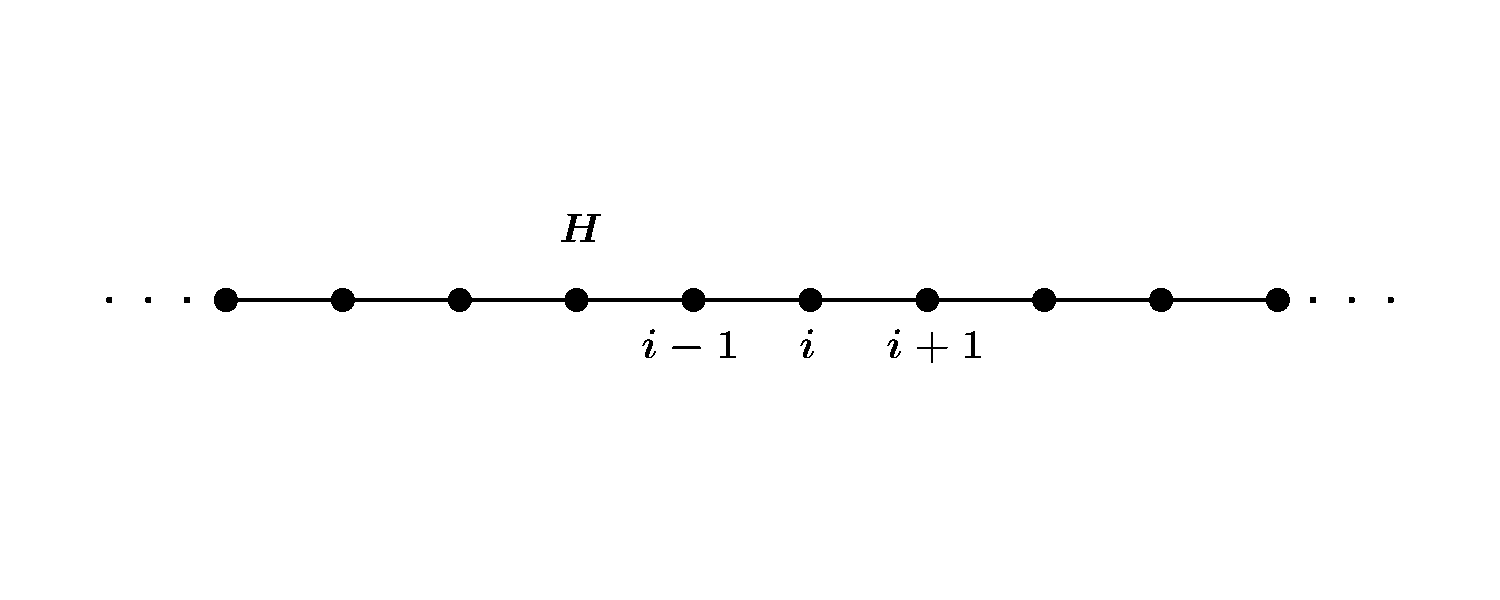
\includegraphics[width=\textwidth]{Imagenes/Models/TB_example.pdf}\vspace{-1.5cm}
        \caption{Red cristalina unidimensional de átomos de hidrogeno}
        \label{fig:Hidrogen_chain}
    \end{figure}
    
    Supongamos que tenemos una red unidimensional cristalina de átomo de hidrogeno que se acomodan sobre una línea recta, como se muestra en la figura(\ref{fig:Hidrogen_chain}). Los traslapes de los orbitales localizados entre vecinos cercanos ayudan al electrón a deslocalizarse de una celda a otra, saltando de un átomo a otro, este potencial de salto está dado por el potencial de traslape o \textit{hopping} entre dos sitios, denotado por $\gamma_{i,j}$, para este sistema el hamitoniano de amarre fuerte está dado por:

    \begin{equation}
        \label{HidrogenoTBH}
        H =  -\sum_{i}\sum_{\langle i, j \rangle } \gamma_{ij} \ket{i}\bra{j}
    \end{equation}
    donde la primera suma es sobre el índice de la celda y la segunda suma es sobre los vecinos cercanos del átomo en la celda unitaria.
    
    Dado que tenemos un sistema periódico, empezaremos escribiendo el operador de traslación $T = \ket{i}\bra{i+1}$ el cual denota la traslación del sitio $i$ al $i+1$, si asumimos que los términos de {\it hopping} dependen únicamente de la distancia entre dos sitios, entonces, $\gamma_{i,i+n} \equiv \gamma_{n}$, entonces ahora podemos escribir el Hamiltoniano de la ecuación \ref{HidrogenoTBH} en función del operador de traslación como $H = -\sum_n \gamma_n T_n$, notemos que ahora es posible diagonalizar el hamiltoniano en la base del operador de traslación, la cual sabemos esta compuesta por los estados de onda plana definidas como:

    \begin{equation}
        \ket{k} = \frac{1}{\sqrt{N}} \sum_j e^{ikj} \ket{j} 
    \end{equation}
    con $k \in \{-\pi/a\,,\,\pi/a\}$.
    
    Si vemos la acción del operador $T^n$ sobre $\ket{k}$ tenemos $T^n \ket{k} =  e^{-ikna}\ket{k}$ 
    por lo tanto la solución al espectro de energías de la ecuación $H(k)\ket{k} = E(k)\ket{k}$, recordando que solo se toma la interacción a primeros vecinos, esta dada por:
    \begin{equation}
        E(k) = 2\gamma \cos(ka)
    \end{equation}
    
\section{Modelo Su-Schrieffer-Heeger (SSH)}
    

El modelo de Su-Schrieffer-Heeger (SSH) es un modelo de amarre fuerte (TB) que describe un electrón sin espín en una celda unitaria con dos sitios en un red unidimensional, un sitio etiquetado por $A$ y otro por $B$ (fig \ref{fig:SSH_Fig}). Las interacciones entre los electrones no son consideradas y la dinámica de los electrones esta descrita por el Hamiltoniano de una sola partícula (\ref{eq:Hamiltonian_ssh}).

\begin{figure}[h!]
    \centering
    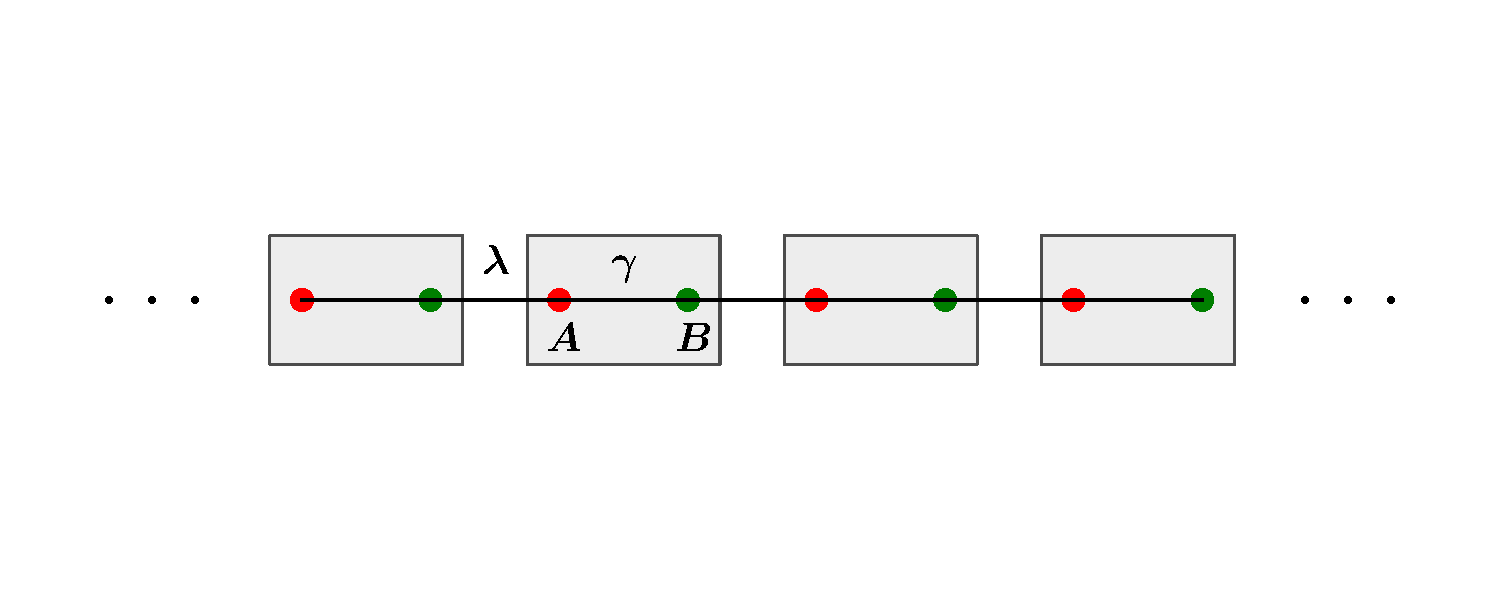
\includegraphics[width=\textwidth]{Imagenes/Models/SSH_example.pdf}\vspace{-1.5cm}
    \caption{Modelo SSH para una cadena de poliacetileno, con una calda unitaria conformada por dos sitios $A$ y $B$, conectadas por parametros de salto intracelda ($\gamma$) e intercelda ($\lambda$)}
    \label{fig:SSH_Fig}
\end{figure}


\begin{equation}
    \label{eq:Hamiltonian_ssh}
    H = \gamma \sum_{i=1}^N (\ket{i,A}\bra{i,B} \,+\, h.c. ) + \lambda \sum_{i=1}^{N-1} (\ket{i + 1,A}\bra{i,B} \,+\, h.c. ) 
\end{equation}

Donde $\bra{i,A}$ y $\bra{i,B}$ denotan el estado de la cadena donde el electrón se encuentra en el i-sima celda , con $i \in {1,2,...,N}$ y en el sitio $A$ o $B$, respectivamente. El parametro de salto intracelda esta dado por $\gamma$ y el intertcelda por $\gamma$. El sumando $h.c.$ representa el hermitiano conjugado.

La matriz del modelo SSH para una cadena con $N = 4$ celdas unitarias en el espacio real, se ve como la ecuación \ref{eq:Hamiltonian_ssh_real}.

\begin{equation}
    \label{eq:Hamiltonian_ssh_real}
    H = 
     \begin{pmatrix}
            0 & \gamma & 0 & 0 & 0 & 0 & 0 & 0 \\
            \gamma & 0 & \lambda & 0 & 0 & 0 & 0 & 0 \\
            0 & \lambda & 0 & \gamma & 0 & 0 & 0 & 0 \\
            0 & 0 & \gamma & 0 & \lambda & 0 & 0 & 0 \\
            0 & 0 & 0 & \lambda & 0 & \gamma & 0 & 0 \\
            0 & 0 & 0 & 0 & \gamma & 0 & \lambda & 0 \\
            0 & 0 & 0 & 0 & 0 & \lambda & 0 & \gamma \\
            0 & 0 & 0 & 0 & 0 & 0 & \gamma & 0 \\
            
        \end{pmatrix}
\end{equation}

Suponiendo que nuestro sistema tiene periodicidad posicional, podemos utilizar el teorema de Bloch $\Psi_{n,k}(\mathbf{r}) = e^{i k\mathbf{r}} u_{n,k}(\mathbf{r})$ con:
\begin{equation}
    H(k + 2\pi) = H(k) ; \,\,\,\,\,\,\,\, \ket{u(k + 2\pi)} = \ket{u(k)} 
\end{equation}


de tal forma que la ecuación de Shrödringer definida por el hamiltoniano escrito en el espacio de momentos para el cuerpo de la cadena, esta dado por:

\begin{equation}
    \label{eq:Hamiltonian_ssh_bloch}
    H =      
     \begin{pmatrix}
            0 & \gamma + \lambda e^{-ik}  \\
            \gamma + \lambda e^{ik} & 0  \\
        \end{pmatrix} ; \,\,\,\, H(k) \begin{pmatrix}
            a(k)   \\
            b(k)  \\
        \end{pmatrix} = E(k) \begin{pmatrix}
            a(k)   \\
            b(k)  \\
        \end{pmatrix}
\end{equation}

Esta forma simplifica mucho el calculo de los invariantes topológicos que definen los estados electrónicos de estos aislantes topológicos.


\begin{figure}[h!]
     \centering
    \captionsetup[sub]{font=small}

     \begin{subfigure}[b!]{0.27 \textwidth}
         \caption{}
         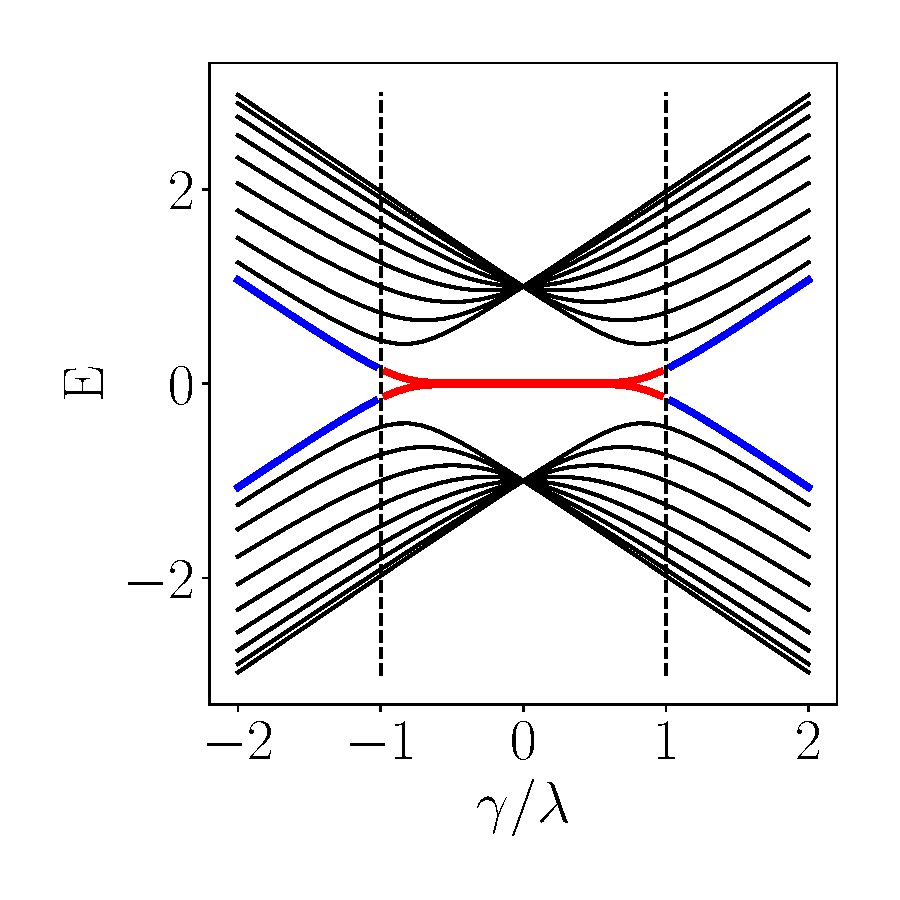
\includegraphics[width=\textwidth]{Imagenes/Shh_images/bands_shh.pdf}
     \end{subfigure}\hspace*{-0.9em}
     \begin{subfigure}[b!]{0.27 \textwidth}
         \caption{}
         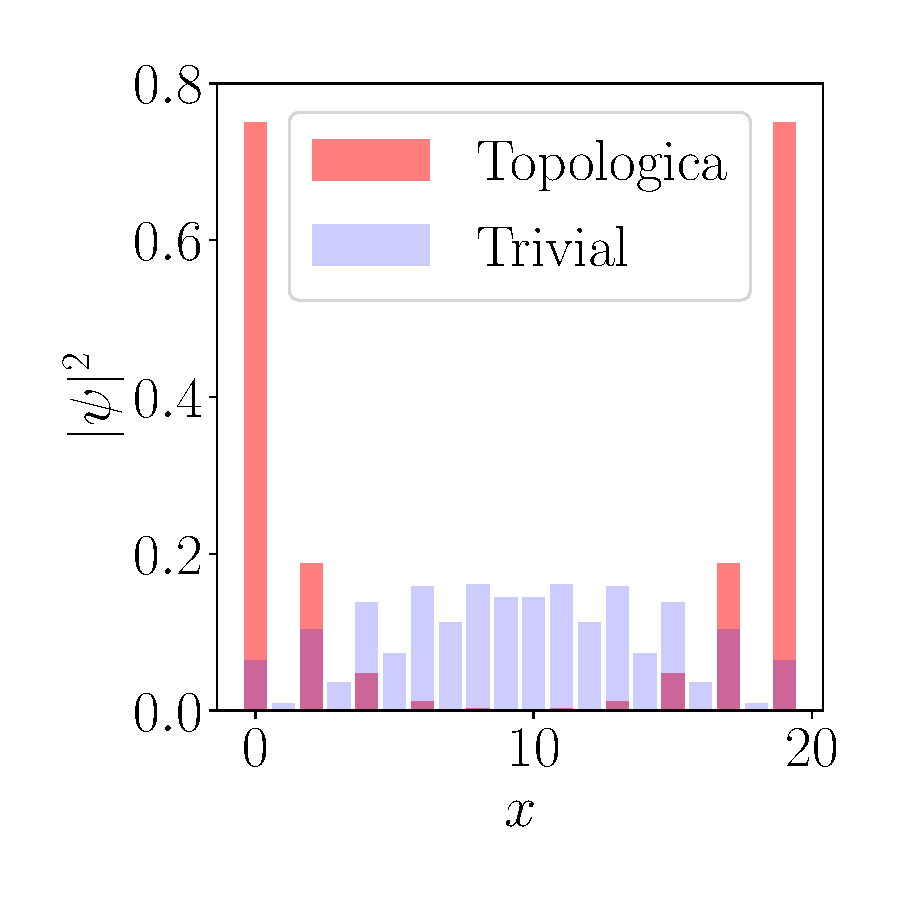
\includegraphics[width=\textwidth]{Imagenes/Shh_images/proyection_ssh.pdf}
     \end{subfigure}\hspace*{-0.9em}
     \begin{subfigure}[b!]{0.27 \textwidth}
         \caption{}
         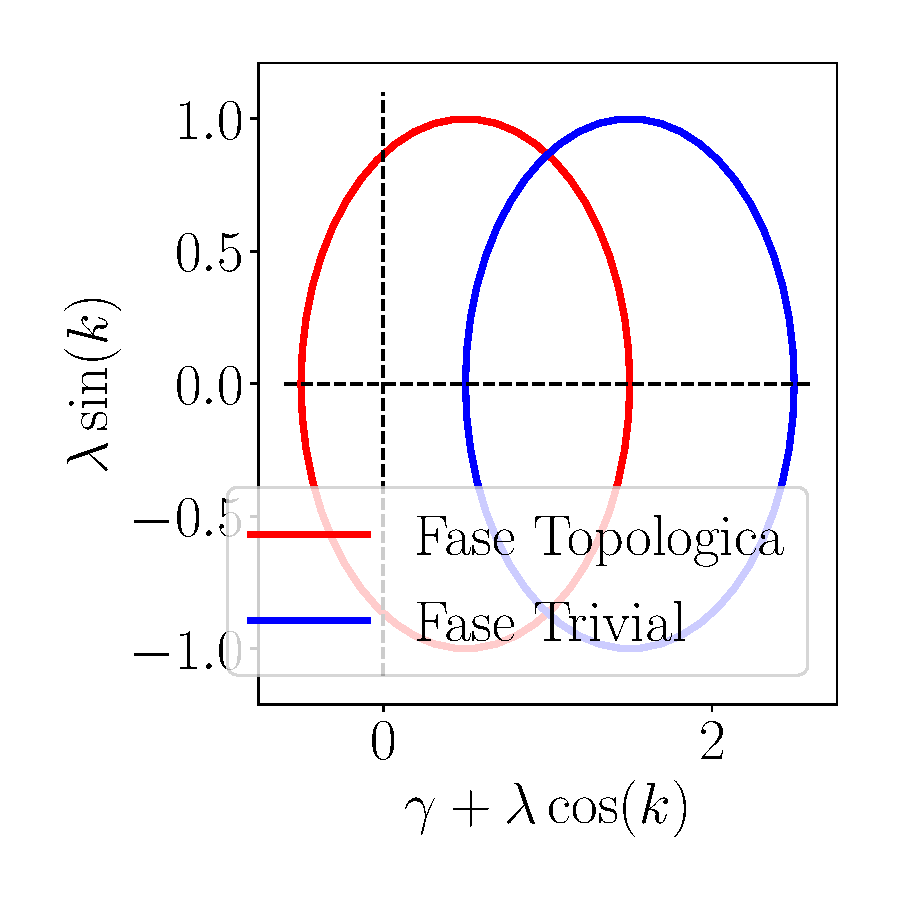
\includegraphics[width=\textwidth]{Imagenes/Shh_images/loop_shh.pdf}
     \end{subfigure}\hspace*{-0.9em}
     \begin{subfigure}[b!]{0.27 \textwidth}
         \caption{}
         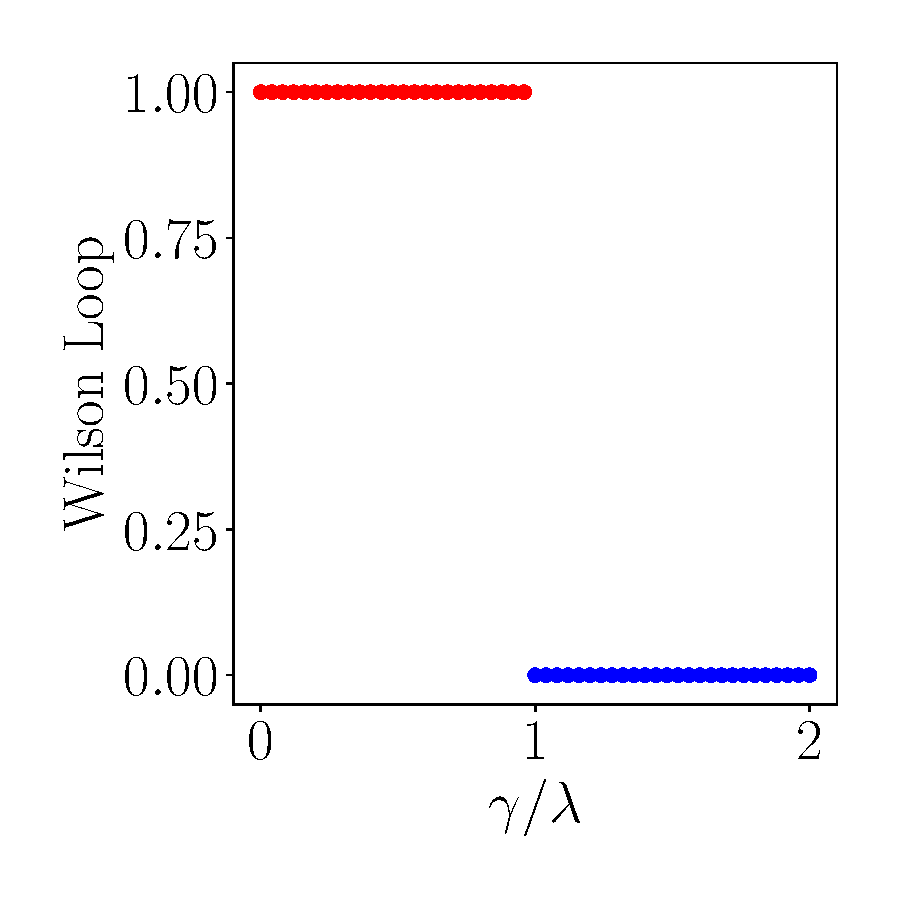
\includegraphics[width=\textwidth]{Imagenes/Shh_images/winding_shh.pdf}
     \end{subfigure}
        \caption{\textbf{(a)} Variación del espectro de energias conforme cambian los parámetros de salto $\gamma/\lambda$. \textbf{(b)} Proyección de la densidad de probabilidad de los estados de borde en la fase topológica (rojo) y en la fase trivial (azul). \textbf{(c)} Representación grafica del número de Winding con valor $1$ en fase topológica (rojo) y $0$ en la fase trivial (azul). \textbf{(d)} Fase de Berry dependiente de los parametros de salto $\gamma/\lambda$ con valor $1$ en fase topológica (rojo) y $0$ en la fase trivial (azul)}.
        \label{fig:SSH_Img_Results}
\end{figure}

Al resolver el sistema de los hamiltonianos (\ref{eq:Hamiltonian_ssh_real}) y (\ref{eq:Hamiltonian_ssh_bloch}) obtenemos los resultados de la figura (\ref{fig:SSH_Img_Results}), en \textbf{(a)} tenemos el comportamiento del espectro de energías conforme los parámetros de salto cambian, las lineas negras corresponden a las energías del cuerpo o bulto de la cadena y las lineas rojas con azul muestran las energías de borde que aparecen debido a la finitud de la cadena y son las energias mas cercanas a la energia de Fermi, Notemos que para los parametros de salto $|\gamma/\lambda|<1$ las energías de los estados de borde se localizan en la energía de Fermi, a estos estados se le conoce como estados topológicos o fase topológica, al proyectar la densidad de probabilidad de los estados correspondientes a estas energías en el espacio real (fig \ref{fig:SSH_Img_Results} \textbf{(b)}), obtenemos para el los parámetros entre los que $\gamma/\lambda < 1$ tenemos la densidad principalmente concentrada en los extremos del material, lo que indicaría un estado de polarización de la cadena, por otro lado, para el los parámetros $|\gamma/\lambda| > 1$ se puede ver en la proyección de los estados de borde la densidad de probabilidad esta distribuida uniformemente en la cadena, como un aislante común, a este estado se le conoce como fase trivial.

Una forma de estudiar el comportamiento de los estados topológicos y triviales de esta cadena, es a través de la información que se puede obtener de la relación de dispersión. 

Supongamos que el hamiltoniano de Bloch de nuestro modelo se puede escribir como una combinación lineal de las matrices de Pauli:

\begin{equation}
    H(k) = d_0(k) \hat{\sigma_0} + d_x(k) \hat{\sigma_x} + d_y(k) \hat{\sigma_y} + d_z(k) \hat{\sigma_z} = d_0(k) \hat{\sigma_0} + \mathbf{d_0}(k) \mathbf{\hat{\sigma_0}}
\end{equation}

Para el modelo SSH, tenemos que:
\begin{equation}
  d_0(k) = 0 ,\; d_x(k) = \gamma + \lambda \cos(k) , \; d_y(k) = \lambda \sin(k), \; d_z(k) = 0  
\end{equation}

La estructura interna de los estados con momento $k$ esta dada por la dirección del vector $\mathbf{d}(k)$, como el numero de onda $k  \in \left[ 0, \; 2\pi \right]$, la ruta que traza $\mathbf{d}(k)$ es un circuito cerrado de radio $\lambda$ en el plano $dx, \,dy$ y centrado en el punto $(\gamma, 0)$. Para que este hamiltoniano describa un aislante es necesario que los círculos que se forman no incluyan el origen\cite{Asboth2015}. La topología de estos ciclos pueden ser caracterizados por un entero, que cuenta el numero de veces que el ciclo rodea el origen, esta cantidad es conocida como el numero de Winding, que es un invariante topológico.

Para el modelo SSH el numero de Winding puede ser 0 o 1, dependiendo de los parámetros, como se puede ver en la \ref{fig:SSH_Img_Results} \textbf{(c)}, donde se puede notar mas a detalle como los ciclos encierran o no el origen dependiendo de los parametros, cambiando las el estado del material entre topológico (rojo) y el trivial (azul). Sin embargo el numero de Winding no es el único numero que caracteriza la topología de la cadena de poliacetileno, en la figura \ref{fig:SSH_Img_Results} \textbf{(d)} se puede observar el comportamiento de la fase de Zak o fase de Berry, que es un invariante topológico que surge de la observación del cambio de fase de la funciones de bloch conforme se recorre de manera cíclica la zona de Brillouin. Este invariante describe como los estados, cuando son topologicos, ganan una fase de $\pi$, es decir, los estados no regresan a su estado inicial después de un ciclo. La Fase de Zak como otros invariantes, es un caso particular de la fase de Berry.

\section{Invariantes topológicos (Fase de Berry)}

Se le llama Invariante topológico a cualquier numero que caracterice a el hamiltoniano de un aislante y que no cambie a través de variaciones adiabáticas. Como consecuencia de estará variaciones el invariante topológico cumple con dos características claves:
\begin{itemize}
    \item Solo esta bien definido en el limite termodinámico.
    \item Depende de las simetrías que se tengan que respetar.
\end{itemize}

Donde se entiende por variación adiabática que los parámetros cambian de forma continua , las simetrías mas importantes del sistema se mantienen y que el gap del bulto o cuerpo de la geometría que están cerca de las energías $E=0$ permanezca abierto.

Existe un gran numero de invariantes topológicos que caracterizan diferentes propiedades físicas de las estructuras geométricas de los materiales, por ejemplo: el numero de Winding, la cantidad de estados de borde, el Willson loop, el numero de Chern, la fase de Berry, etc. Para los fines de este trabajo hablaremos de la fase de Berry, la cual recientemente a sido asociada como responsable de una gran gamma de fenómenos interesantes en las propiedades de los materiales, tales como la ferroelectricidad, el magnetismo orbital, el efecto hall cuantico, el bombeo de cargas y la polarización.

En mecánica cuántica la función de onda normalmente se define con una fase que no tiene sentido físico ya que desaparece al tomar el valor de expectación. Sin embargo la fase de Berry mostró en 1984 que esta fase tiene efectos físicos observables si el sistema se transforma de manera adiabática y cíclica. En ausencia de degeneración, el sistema regresara este mismo punto al cerrar el ciclo, pero habrá una diferencia de fase igual a la integral temporal de la energía mas un termino extra que es lo que conocemos como fase de Berry.

Consideremos un sistema general descrito por el hamiltoniano $H(\mathbf{\lambda})$, donde $\mathbf{\lambda}$ es un conjunto de parámetros que evolucionan en el tiempo, $\mathbf{\lambda} = \left( \lambda_1(t), \lambda_2(t),\dots, \lambda_n(t)\right)$. Tambien introduciomos una base ortonormal de estados en cada punto de $\lambda$ del espacio, $\ket{n(\lambda(t))} = \ket{n(\lambda)}$, tal que:
\begin{equation}
    H(\lambda) \ket{n(\lambda)} =  E_n\ket{n(\lambda)}
\end{equation}
De acuerdo con el teorema adiabatico, un sistema que se encuentra inicialmenten en el estado $\ket{n(\lambda_0)}$ permanecera como un eigenestado instantaneo de $H(\lambda)$ para todo $t$, entonces:
\begin{align}
    \ket{\psi(t)} =  e^{i\theta_n(t)}\ket{n(\lambda)}
\end{align}

Introduciendo la ecuacion anterior en la ecuacion de Shrodringer:
\begin{align}
    (H(\lambda) - \partial_t) e^{i\theta_n(t)}\ket{n(\lambda)} =  0
\end{align}

Desarrollando es fácil obtener la ecuación diferencial para $\theta$:

\begin{align}
    \dot{\theta} = \frac{1}{\hbar} E_n(\lambda) - i \sandwich{n(\lambda)}{\partial_t}{n(\lambda)}
\end{align}

La expresion final para la fase se obtiene integrando en el tiempo:

\begin{align}
   \theta = \frac{1}{\hbar} \int_t E_n(\lambda) d\lambda - i \int_t \sandwich{n(\lambda)}{\partial_t}{n(\lambda)} d\lambda
\end{align}

Notemos que el primer sumando es la fase dinámica usual, mientras el segundo termino es denominado como la fase de Berry:
\begin{align}
    \gamma := i \int_{\lambda(0)}^{\lambda(t)} \sandwich{n(\lambda)}{\partial_\lambda}{n(\lambda)} d\lambda
\end{align}

Donde el termino $A_n = \sandwich{n(\lambda)}{\partial_\lambda}{n(\lambda)}$ es conocido como la conexión de Berry. Si usamos el Teorema de Stokes, si integramos sobre una superficie cerrada $C$ que se puede parametrizar en el tiempo:

\begin{align}
    \gamma_n = \oint_C A_n \cdot d\lambda = \int_S \nabla_\lambda \times A_n \cdot dS_\lambda
\end{align}


Donde al vector $\Omega_n = \nabla_\lambda \times A_n$ se le conoce como curvatura de Berry. Se sabe que la integral de la curvatura de Berry sobre un superficie cerrada, tal como un esfera o un toro, es topológica y esta cuantizada; a estos números cuánticos topológicos se les denomina números de Chern.

\subsection{Polarización, centros de Wannier y Fase de Berry}

En los textos de electromagnetismo la polarización macroscópica se define como la cantidad de dipolos eléctricos por unidad de volumen, donde los dipolos son pequeñas unidades polarizadas, en la simplificación del problema se asume que la distribución de carga entre los dipolos eléctricos es nula. Sin embargo, al estudiar la densidad electrónica de un material polarizado a través de la mecánica cuántica podremos notar que la carga no esta divida en paquetes convenientes y que la unidad de polarización no existe. 

\begin{figure}[tbh!]
    \centering
   \captionsetup[sub]{font=small}
    \begin{minipage}[h!]{1\textwidth}
        \begin{subfigure}[b!]{1 \textwidth}
            \caption{}
            \vspace*{-2em}
            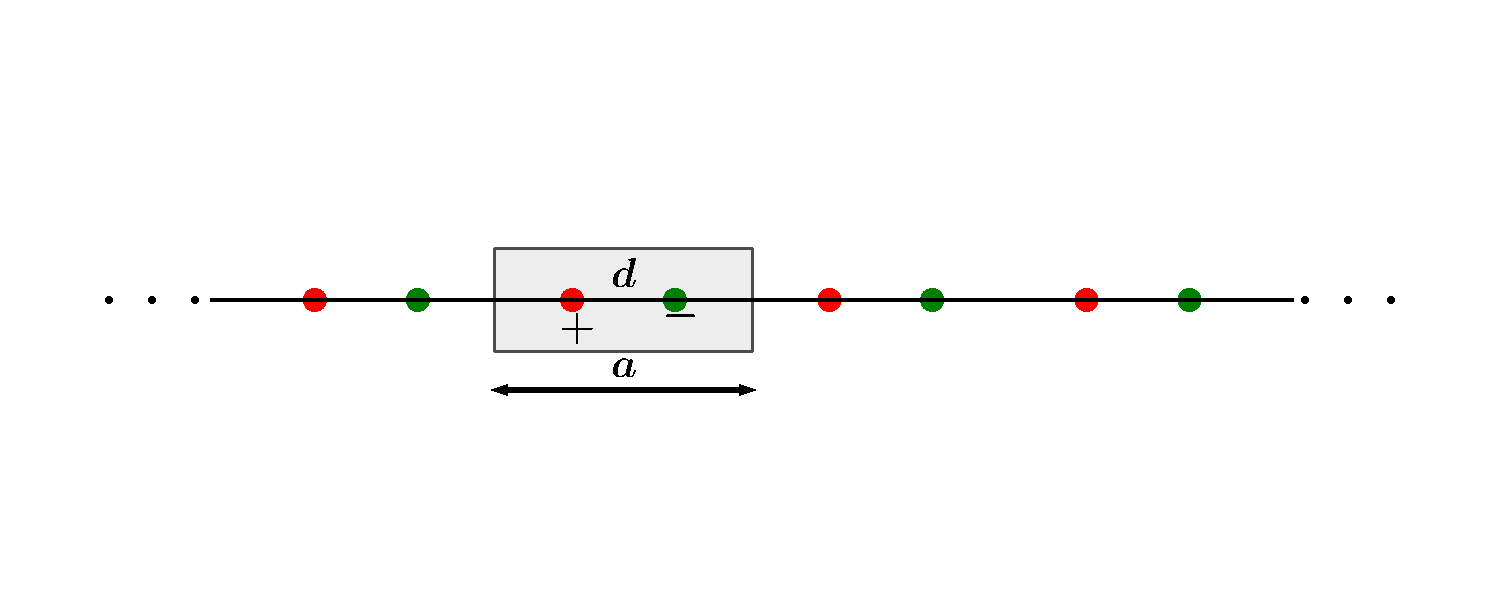
\includegraphics[width=\textwidth]{Imagenes/Models/polarizatio_example_a.pdf}
        \end{subfigure}\hspace*{-0.5em}
    \end{minipage}\vspace*{-2.5em}

    \begin{minipage}[h!]{1\textwidth}
        \begin{subfigure}[b!]{1 \textwidth}
            \caption{}
            \vspace*{-2em}
            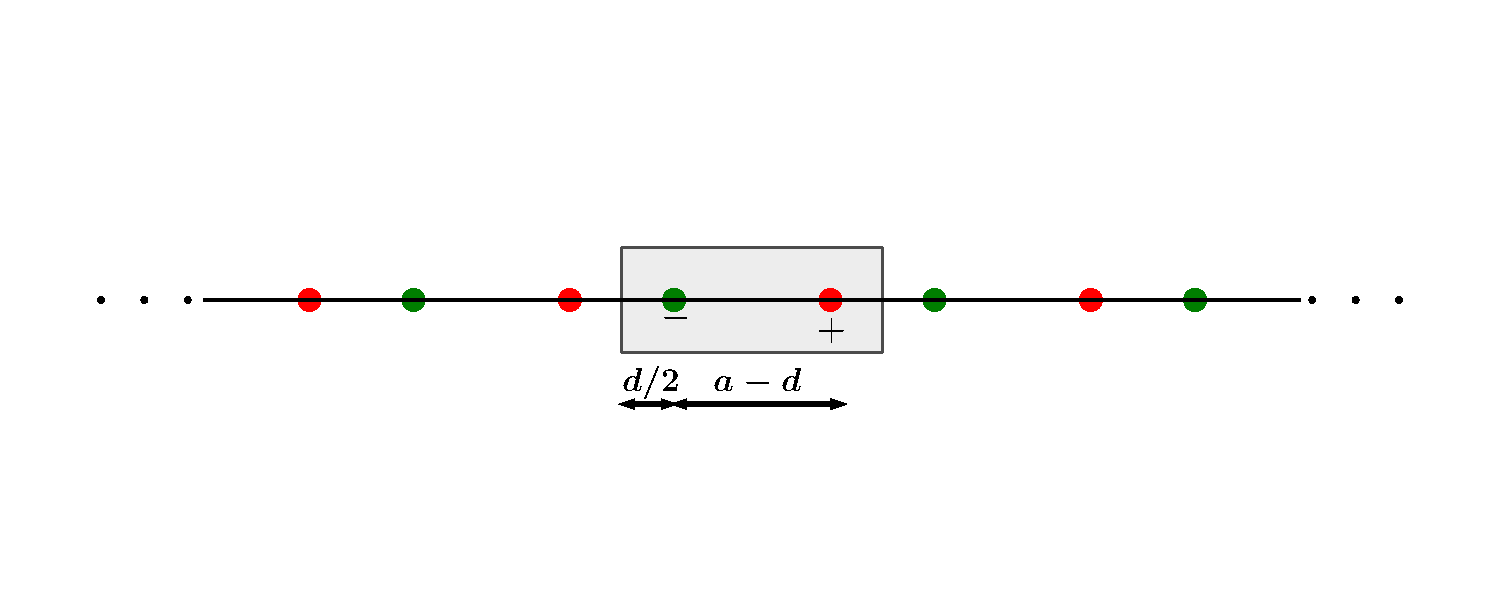
\includegraphics[width=\textwidth]{Imagenes/Models/polarizatio_example_b.pdf}
        \end{subfigure}\hspace*{-0.5em}
    \end{minipage}\vspace*{-1.5em}
    
    \caption{Red cristalina infinita periódica conformada por una molécula dicotómica anión (verde), catión (rojo), separados por una distancia \textbf{(a)} $d$ o \textbf{(b)} $a-d$, dependiendo la elección de celda.}
    \label{fig:Model_polarization}
\end{figure}

Una aparente solución podría ser contar los momentos dipolares como una integral continua sobre la densidad electrónica, sin embargo esta solución es solo aparente, pues esta cantidad depende de como se seleccione la celda sobre la cual se integra, este detalle podría darnos cantidades distintas para para diferentes elecciones de celda, es decir, conocer la densidad electrónica no es información suficiente para determinar la polarización en una red aislante cristalina.
\begin{equation}
\label{polarization_classic}
\textbf{P} = \frac{1}{V_{cell}}\int_{cell} \textbf{r} \rho(\textbf{r})d^3r
\end{equation}

por ejemplo:

Supongamos que tenemos una red cristalina periódica conformada por una molécula dicotómica que se repite indefinidamente formando una cadena infinita, la molécula esta formada por un anión y un catión, ambos separados a una distancia $d$ y la celda unitaria tiene una distancia $a$ (fig \ref{fig:Model_polarization} \textbf{(a)}). Si calculamos la polarización con la expresión \ref{polarization_classic} obtendremos la ecuación \ref{eq:pol1}.

\begin{equation}
    \label{eq:pol1}
    P_1 = \frac{qd}{a}
\end{equation}

Ahora supongamos que la selección de la celda unitaria es de la misma longitud pero con una posición diferente, como se muestra en la (fig \ref{fig:Model_polarization} \textbf{(b)}), al calcular la polarización obtenemos la ecuación \ref{eq:pol2}.

\begin{equation}
    \label{eq:pol2}
    P_2 = \frac{qd}{a} + q
\end{equation}

Si nos tomamos todas las posibles elecciones de celdas llegaremos a la conclusión de que la expresión en general de la polarización estara dada por las expresiones \ref{eq:pol_gral1d} y \ref{eq:pol_gral3d}.

\begin{equation}
    \label{eq:pol_gral1d}
    P = P_o + nq\,\,  {\rm con} \,\,n \in \mathbb{Z}\,\, \text{para el caso 1D} 
\end{equation}

\begin{equation}
    \label{eq:pol_gral3d}
    P = P_o + n\frac{qR}{V}\,\,  \text{con} \,\,n \in \mathbb{Z}\,\, \text{para el caso 3D}
\end{equation}

Donde $P_o$ es la polarización electrónica cuando se escoge convenientemente una celda centrosimétrica, $q$ es la carga de los iones, $R$ es la magnitud del vector de la celda y V es el volumen de la celda.

Como podemos notar, la polarización está multivaluada para diferentes elecciones de celda, donde la polarización difiere entre si en un termino $P_q = \frac{qR}{V}$ el cual es conocido como \textit{``cuanto de polarización''}.

¿Pero que significa esta cantidad? Imaginemos que en nuestro sistema se mueve un electrón de un anión de una celda a otra, ¿Cómo cambia la polarización debido al transporte de carga? La respuesta es $\Delta P = \frac{-ea}{V}$, es decir, como consecuencia de la periodicidad del sistema, el mover un electrón de una celda a otra deja a el sistema físico exactamente igual, pero a la polarización no.

Veamos entonces un ejemplo de transporte de carga. Supongamos una evolución adiabática en el cuerpo de un aislante cristalino, donde el cambio de la polarización estará dado por:

\begin{equation}
    \Delta \textbf{P} = \int_i^f \textbf{J}(t)dt
\end{equation}
Si \textbf{P} estuviera únicamente definida para cualquier ciclo cerrado, implicaría que  $\Delta \textbf{P} = 0$. Ahora supongamos que tenemos una onda de densidad de carga que se desliza por un aislante cristalino uni-dimensional, el hamiltoniano de este modelo está dado por:
\begin{equation}
    H =  \frac{p^2}{2m} - V_0 cos(\frac{2\pi x}{a} - \lambda)
\end{equation}
Donde $a$ es la constante de la red y $\lambda$ es un parámetro de ciclo el cual varia con el tiempo y corre de $0$ a $2\pi$. 
Supongamos que $V_o$ es suficientemente grande para contener a una partícula semiclásica con carga $-e$ atrapada en el potencial al rededor de el mínimo del potencial ($x = \frac{a\lambda}{2\pi}$). Después de un ciclo, la partícula será bombeada de tal forma que:

\begin{equation}
    \Delta \textbf{P}_{cyc} = \oint \textbf{J}(t)dt = -e
\end{equation}

Por lo tanto el bombeo de la carga es inconsistente con la idea de que la polarización es únicamente  definida. 

Pero ahora ¿Como calculamos esta diferencia de polarización para casos donde las cargas no están localizadas como sucede en los sistemas cuánticos cristalinos donde la carga esta distribuida por todo el cristal? Primero debemos notar que la contribución de los electrones a la polarización es una propiedades del estado electrónico de varios cuerpos, la idea central para contestar esta pregunta es escribir estos estados electrónicos de varios cuerpos usando una base ortonormal  de estados localizados que nos permitan tener una visualización tipo átomo de la densidad electrónica, que comúnmente es una función continua en todo el espació, esta descripción nos permitirá seguir sumando los momentos dipolares como cargas multiplicadas por sus posiciones. La base de estados que permitirá todo esto es conicidad estados de Wannier. La contribución de cada electrón en un estado Wannier al centro de carga puede evaluarse fácilmente y luego sumarse.

Las funciones de Wannier $w_n(\textbf{r})$ de la n-sima banda, en la celda unitaria asociada a $\textbf{R}$, están definidas como:
\begin{equation}
\begin{split}
     w_n(\textbf{r} - \textbf{R}) &= \frac{\Omega}{(2\pi)^3} \int_{BZ} d^3\textbf{k} e^{-i \textbf{k} \cdot \textbf{R}} \Psi_{n\textbf{k}}(\textbf{r})\\
     &= \frac{\Omega}{(2\pi)^3} \int_{BZ} d^3\textbf{k} e^{i \textbf{k} \cdot (\textbf{r} - \textbf{R})} u_{n\textbf{k}}(\textbf{r})
\end{split}
\end{equation}

A diferencia de las funciones de Bloch que están deslocalizadas en el espacio las funciones de Wannier si están localizadas. Estás son relevantes para este problema porque la naturaleza de la localización proporciona una conveniente descripción de la densidad de carga en un sólido. Si bien sabemos en
realidad de que la densidad de carga en un sólido es una función continua, la idea de que esta puede estar localizada nos permitirá continuar calculando los momentos dipolares sumando sobre cargas multiplicadas por posiciones (Ahora tenemos una manera conveniente de tomar las celdas que permitan esto).
Para esto primero suponemos que la concentración de electrones esta al rededor de la función de Wannier, a esta "posición" de la función de wannier se les llama ``Centros de Wannier", $\overline{\textbf{r}}$ y se calcula como el valor esperado de la posición:
\begin{equation}
\label{eq:Wcenter}
\begin{split}
        \overline{\textbf{r}} &= \sandwich{w_n}{\textbf{r}}{w_n}\\
        &= \int w^*_n(\textbf{r})\,\textbf{r}\, w_n(\textbf{r})\, d^3\textbf{r}
\end{split}
\end{equation}
Como se verá más adelante en el marco teórico, la ecuación \ref{Wcenter} se puede escribir en términos de las funciones periódicas $u_{n\textbf{k}}$ y usando al operador posición en la representación de momentos $\textbf{r} = -i\frac{\partial}{\partial\textbf{k}}$:
\begin{equation}
    \overline{\textbf{r}} = i\frac{\Omega}{(2\pi)^3} \int_{BZ} d^3\textbf{k}\,e^{-i\textbf{k}\cdot\textbf{R}}\braket{u_{n\textbf{k}}}{\frac{\partial u_{n\textbf{k}} }{\partial\textbf{k}}}
\end{equation}

Con el concepto de los centros de Wannier, ahora, la expresión para la polarización se puede escribir como las contribuciones de los iones (ya antes localizados) y las contribuciones debido a las cargas electrónicas centradas, ahora, en los centros de Wannier, para cada banda ocupada.

\begin{equation}
    p = \frac{1}{V_{cell}} (\sum_i (q_i x_i)^{ions} + \sum_n^{occ}(q_n \overline{\textbf{r}})^{WF})
\end{equation}

Es importante recalcar que el segundo termino en la polarización es mejor conocido como como la fase de Berry:
\begin{equation}
    \label{eq:Barry_fase}
    \sum_n^{occ}\int_{BZ} d^3\textbf{k}\,e^{-i\textbf{k}\cdot\textbf{R}}\braket{u_{n\textbf{k}}}{\frac{\partial u_{n\textbf{k}} }{\partial\textbf{k}}}
\end{equation}
Está cantidad será la central en el calculo de invariantes topológicos en estados de polarización que definen a un aislante topológico de alto orden. 


\section{Bombeo Adiabático}

\begin{figure}[h!]
     \centering
    \captionsetup[sub]{font=small}

     \begin{subfigure}[b!]{0.27 \textwidth}
         \caption{}
         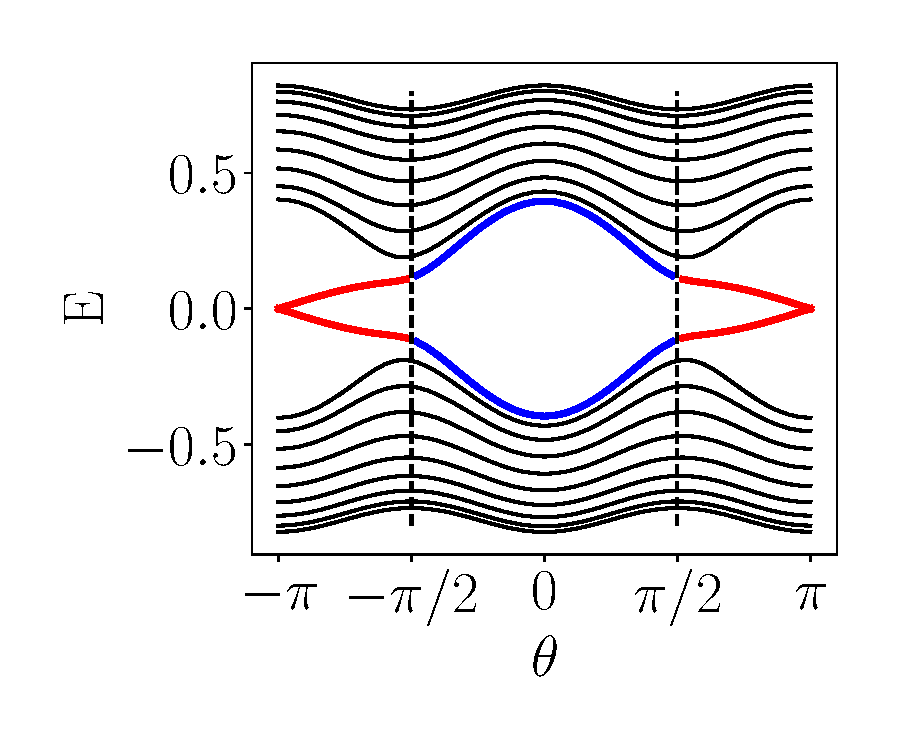
\includegraphics[width=\textwidth]{Imagenes/Shh_images/bands_shh_pump.pdf}
     \end{subfigure}\hspace*{-0.9em}
     \begin{subfigure}[b!]{0.27 \textwidth}
         \caption{}
         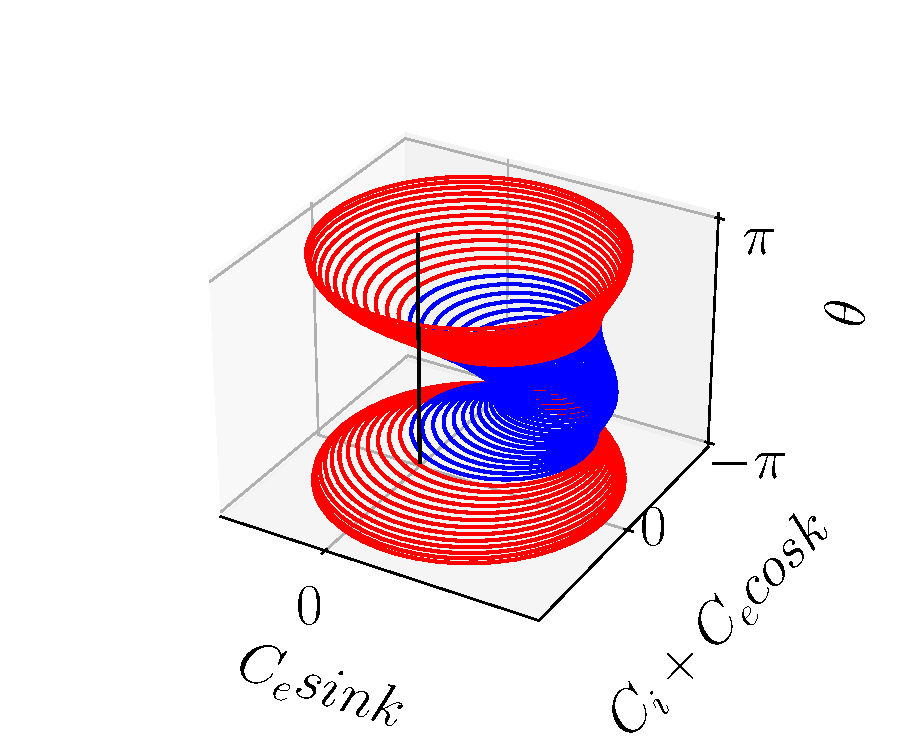
\includegraphics[width=\textwidth]{Imagenes/Shh_images/loop_pump_ssh.pdf}
     \end{subfigure}\hspace*{-0.9em}
     \begin{subfigure}[b!]{0.27 \textwidth}
         \caption{}
         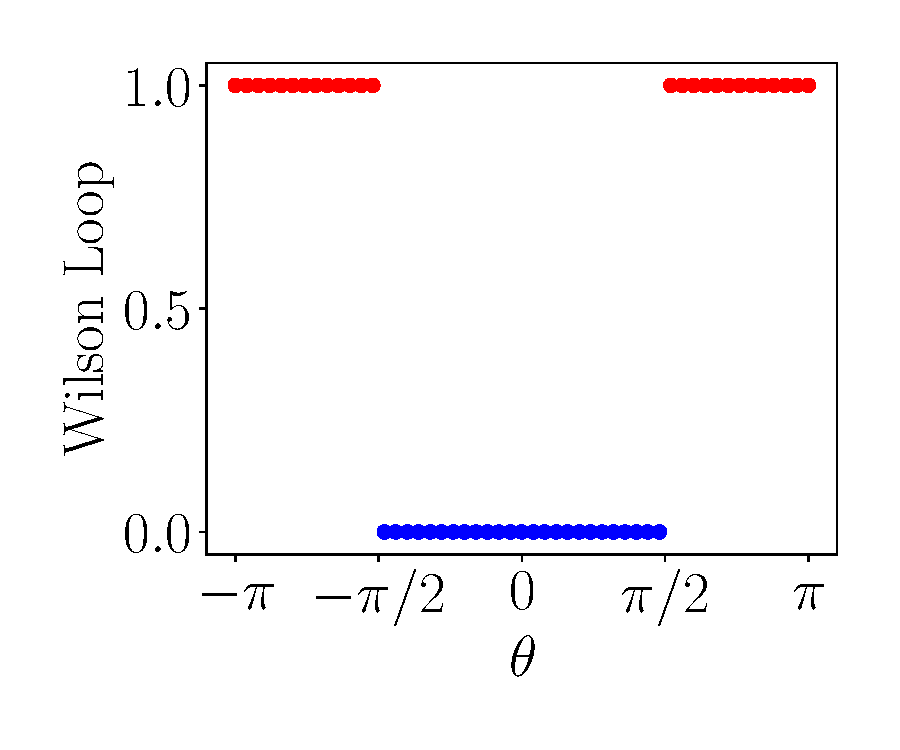
\includegraphics[width=\textwidth]{Imagenes/Shh_images/winding_shh_pump.pdf}
     \end{subfigure}\hspace*{-0.9em}
     \begin{subfigure}[b!]{0.27 \textwidth}
         \caption{}
         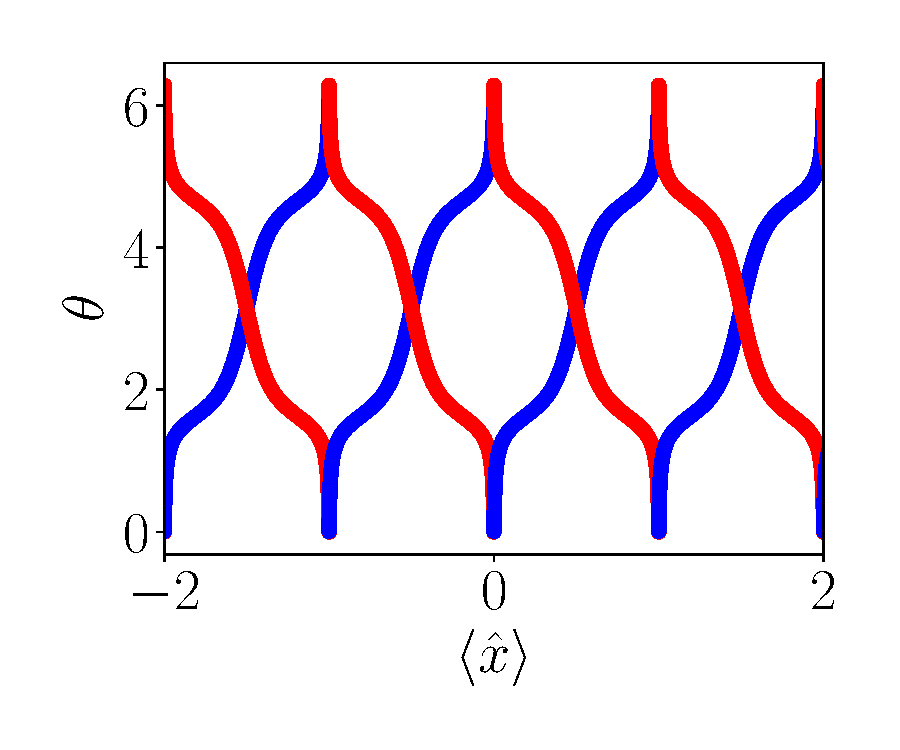
\includegraphics[width=\textwidth]{Imagenes/Shh_images/wannier_center_shh_pump.pdf}
     \end{subfigure}
     \caption{\textbf{(a)} Variación del espectro de energias conforme cambia el parametro ciclico $\theta$. \textbf{(b)} Representacion grafica del número de Winding en la fase topológica (rojo) y en la fase trivial (azul). \textbf{(c)}Fase de Berry dependiente de los parametros de salto $\gamma/\lambda$ con valor $1$ en fase topológica (rojo) y $0$ en la fase trivial (azul) .\textbf{(d)} cambio del valor esperado o centros de wannier conforme varia el parametro ciclico.}
    \label{fig:Pump_example_Results}
\end{figure}

Una de las aplicaciones mas interesantes de la fase de Berry es demostrar que el cambio lento de los parámetros temporales en un solido 1-dimensional puede generar transporte o bombeo de cargas después de recorrer un ciclo.

Recordemos que en el caso del modelo de SSH anterior teníamos parámetros que al variar mostraban cambios en los estados de la geometría estudiada, una forma de poder analizar como suceden estas transiciones de fase es a través del bombeo adiabático, haciendo variar los parámetros de salto del hamiltoniano por medio de un parámetro adiabático y cíclico.

\subsection{Modelo de Rice-Mele}

Consideremos el hamiltoniano de SSH del modelo anterior, con una pequeña modificación, los parámetros de salto variarán en el tiempo a través de un parámetro cíclico $\theta \in \left[ 0 , 2\pi\right]$ y agregaremos un termino de sitio que nos permitirá suavizar los estados de transición:

% \begin{align}
%     \nonumber\gamma \rightarrow C_{int}(\theta) = \gamma\exp(-\beta(-A \cos \theta - 1)) \; &,\;  \lambda \rightarrow C_{ext}(\theta) = \lambda \exp(-\beta( A \cos \theta - 1 )) \;,\; \\  C_{in}(\theta) = \delta \sin \theta
% \end{align}

\begin{align}
    \nonumber\gamma \rightarrow \gamma (\theta) = \gamma_0 e^{\displaystyle-\beta(-A \cos \theta - 1)} \; &,\;  \lambda \rightarrow \lambda(\theta) = \lambda_0 e^{\displaystyle-\beta( A \cos \theta - 1 )} \;,\; \\  \epsilon(\theta) = \epsilon_0 \sin \theta
\end{align}

Con $\epsilon_0$ suficientemente pequeño.

De tal forma que el nuevo modelo estará descrito por el siguiente hamiltoniano de Bloch:
\begin{equation}
    H_k(\theta) =      
     \begin{pmatrix}
            \epsilon(\theta) & \gamma(\theta) + \lambda(\theta) e^{-ik}  \\
            \gamma(\theta) + \lambda(\theta) e^{ik} & -\epsilon(\theta) \\
        \end{pmatrix} 
\end{equation}
Y el hamiltoniano en el espacio real, para una cadena con 4 celdas unitarias:
\begin{equation}
    H (\theta)= 
     \begin{pmatrix}
            \epsilon(\theta) & \gamma(\theta) & 0 & 0 & 0 & 0 & 0 & 0 \\
            \gamma(\theta) & -\epsilon(\theta) & \lambda(\theta) & 0 & 0 & 0 & 0 & 0 \\
            0 & \lambda(\theta) & \epsilon(\theta) & \gamma(\theta) & 0 & 0 & 0 & 0 \\
            0 & 0 & \gamma(\theta) & -\epsilon(\theta) & \lambda(\theta) & 0 & 0 & 0 \\
            0 & 0 & 0 & \lambda(\theta) & \epsilon(\theta) & \gamma(\theta) & 0 & 0 \\
            0 & 0 & 0 & 0 & \gamma(\theta) & -\epsilon(\theta) & \lambda(\theta) & 0 \\
            0 & 0 & 0 & 0 & 0 & \lambda(\theta) & \epsilon(\theta) & \gamma(\theta) \\
            0 & 0 & 0 & 0 & 0 & 0 & \gamma(\theta) & -\epsilon(\theta) \\
            
        \end{pmatrix}
\end{equation}

En la figura \ref{fig:Pump_example_Results} \textbf{(a)}, \textbf{(b)} y \textbf{(c)} se pueden observar diferentes formas de observar la transición de fase entre fase topológica y trivial, en fig.\ref{fig:Pump_example_Results} \textbf{(a)}, se puede ver como en el espectro de bandas el comportamiento de las energías de los estados de borde cambian de tener un gap amplio, es decir una fase trivial, a tener una brecha energética nula o una fase topológica, podemos seguir este cambio a través del numero de winding, en la fig.\ref{fig:Pump_example_Results} \textbf{(b)} como los círculos que forman la relación de dispersión pasan de rodear el origen a no hacerlo, en la fig.\ref{fig:Pump_example_Results} \textbf{(c)} se puede observar un cambio mas abrupto en la transición de fase no trivial, pues este caracteriza la fase que la ecuación de onda gana cuando se recorre un ciclo por la zona de brilluan, esto determina que hay valores en la variación temporal en los que el material ganara una fase y hay otros en los que no. Por ultimo, Si nuestro material gana una fase y traiciona de estado a estado después de en un ciclo, existe un cambio en el? La respuesta es si, a pesar de que el hamiltoniano del material no haya cambiado después de el ciclo, los eigenestados si cambiaron y esto se ve reflejado en un bombeo de cargar a través de la cadena.

\begin{figure}[h!]
    \centering
   \captionsetup[sub]{font=small}

    \begin{subfigure}[b!]{0.2 \textwidth}
        \caption*{$\theta=-\pi$}
        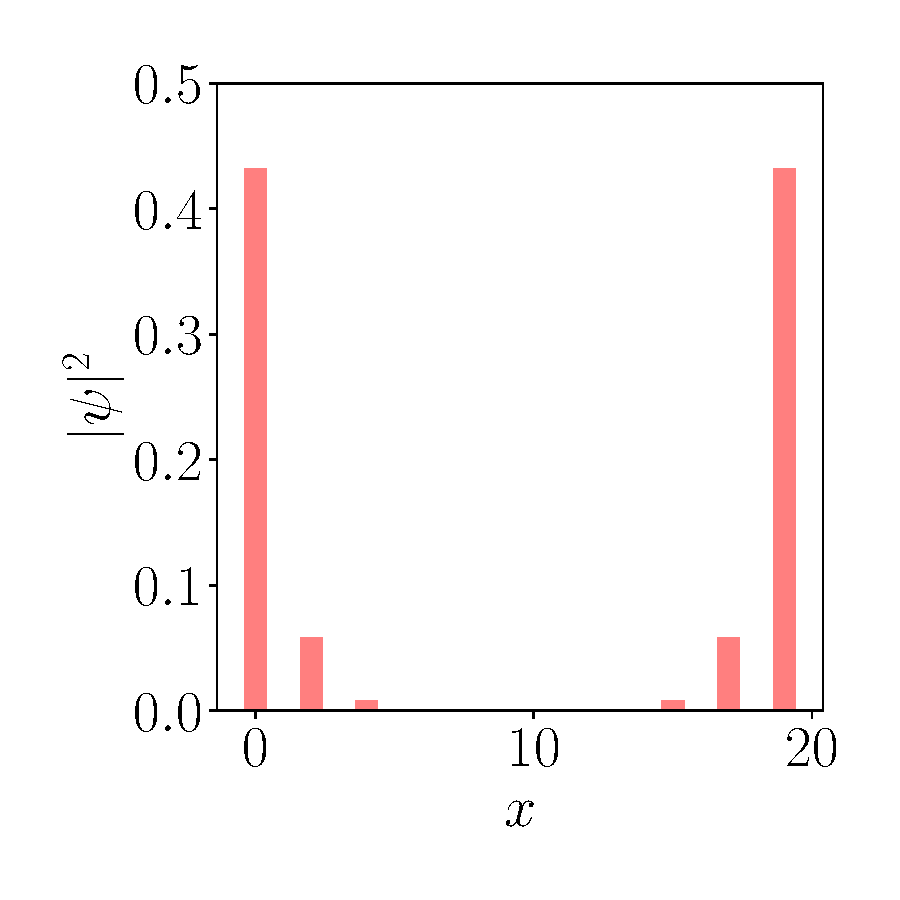
\includegraphics[width=\textwidth]{Imagenes/Shh_images/proyection_0.pdf}
    \end{subfigure}\hspace*{-0.9em}
    \begin{subfigure}[b!]{0.2 \textwidth}
        \caption*{$\theta=-\frac{\pi}{2}$}
        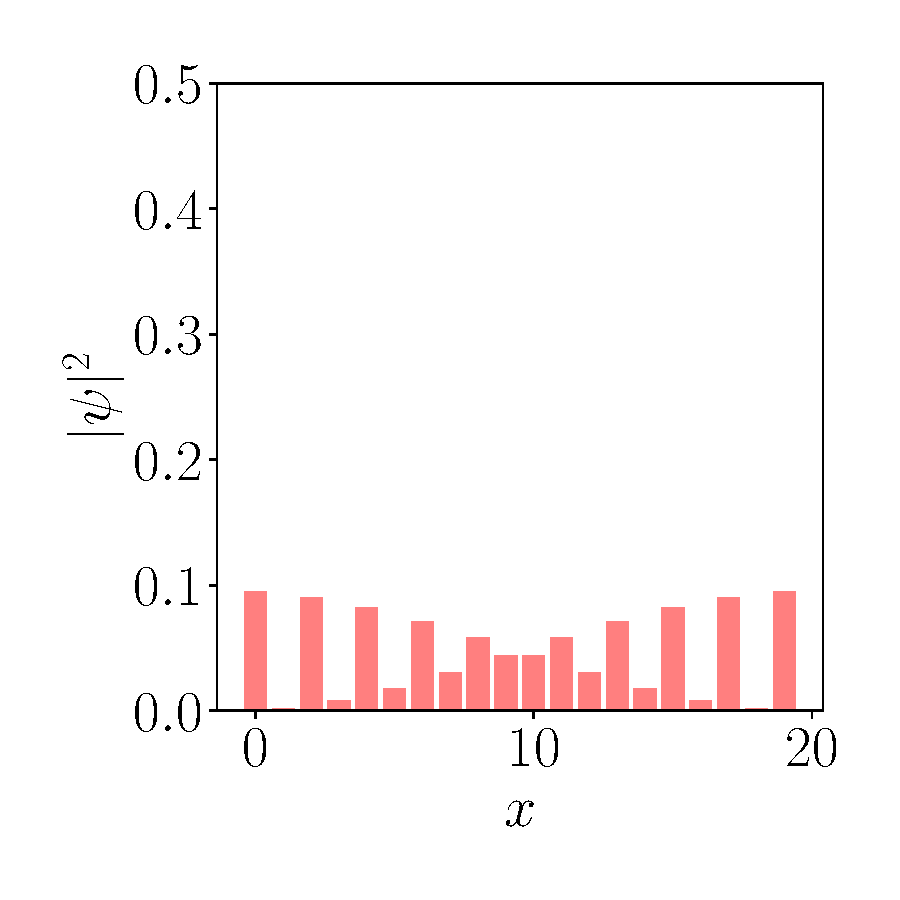
\includegraphics[width=\textwidth]{Imagenes/Shh_images/proyection_1.pdf}
    \end{subfigure}\hspace*{-0.9em}
    \begin{subfigure}[b!]{0.2 \textwidth}
        \caption*{$\theta=0$}
        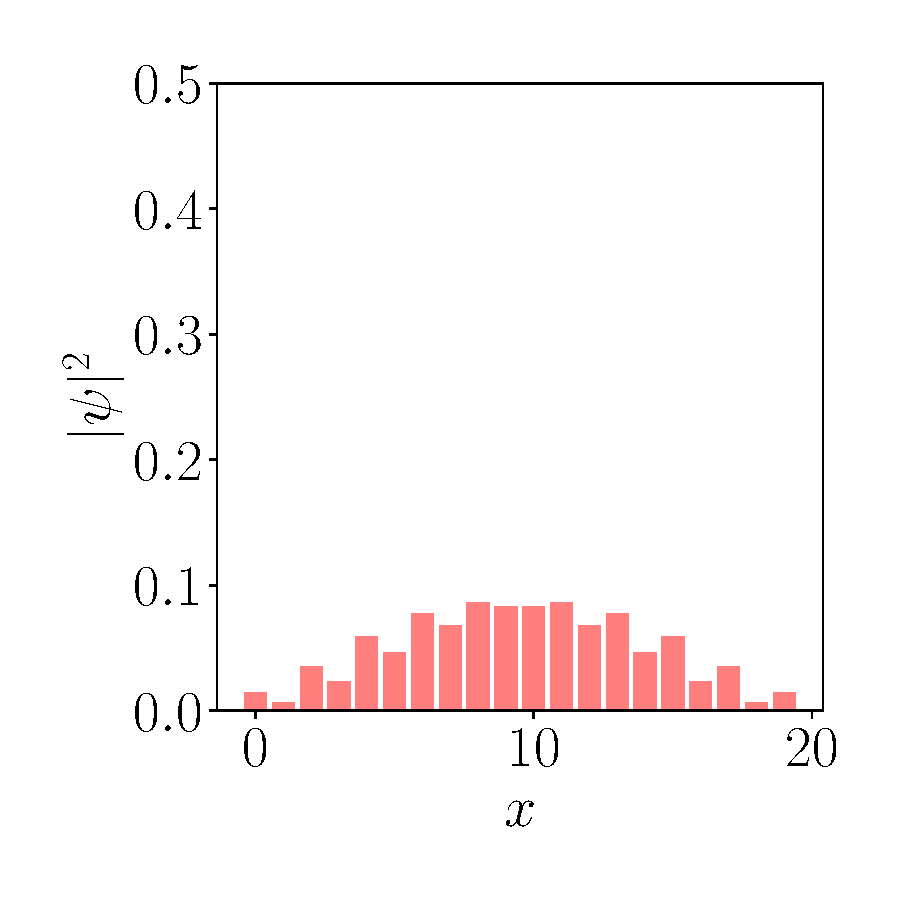
\includegraphics[width=\textwidth]{Imagenes/Shh_images/proyection_2.pdf}
    \end{subfigure}\hspace*{-0.9em}
    \begin{subfigure}[b!]{0.2 \textwidth}
        \caption*{$\theta=\frac{\pi}{2}$}
        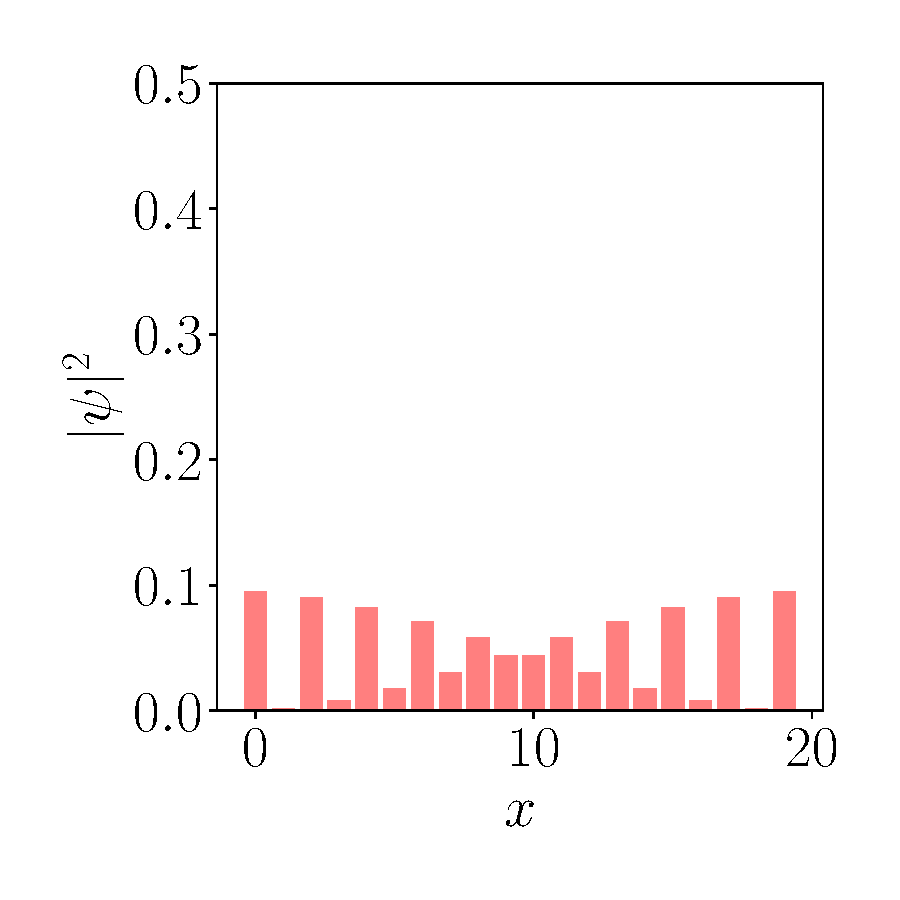
\includegraphics[width=\textwidth]{Imagenes/Shh_images/proyection_3.pdf}
    \end{subfigure}\hspace*{-0.9em}
    \begin{subfigure}[b!]{0.2 \textwidth}
        \caption*{$\theta=\pi$}
        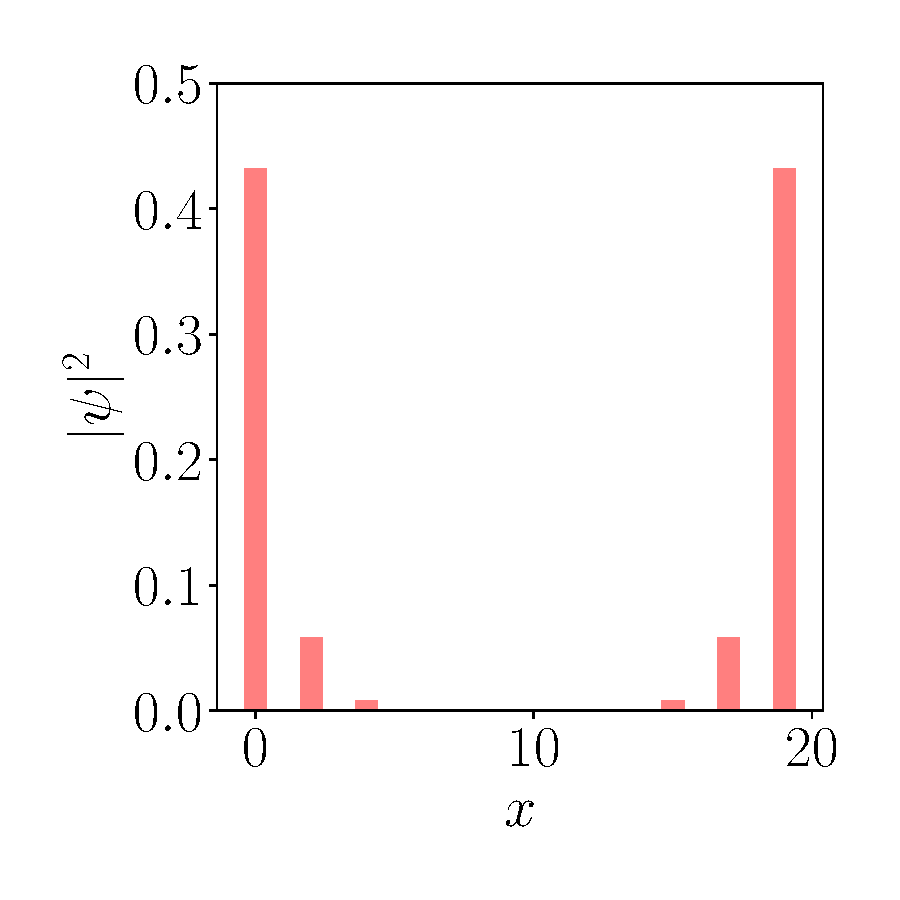
\includegraphics[width=\textwidth]{Imagenes/Shh_images/proyection_4.pdf}
    \end{subfigure}
       \caption{Proyección de los estados correspondientes a las energias negativas mas cernas a los estados de Fermi para distintos valores de $\theta \in [-\pi, \pi]$. }
    \label{fig:pump_RM_proyection}
\end{figure}

Una forma de estudiar esta cuestión es a través de hacer un seguimiento de los centros de wannier de cada celda, si existe un desplazamiento de este centro de celda a celda, la fase que gana nuestro sistema después de un ciclo, se puede interpretar como el desplazamiento de cargas de una celda a otra lo que denotaría que existe un bombeo y como vimos en el capitulo anterior, la corriente generada por este bombeo propicia un estado de polarización en el material, el cual se puede observar cuando proyectamos los estados de las energías centrales de \ref{fig:Pump_example_Results} \textbf{(a)} en el espacio real, fig(\ref{fig:pump_RM_proyection}).


\section{Fractales (Sierpinsky Carpet)}
\label{sc:Fractales}

\begin{figure}[h!]
     \centering
    \captionsetup[sub]{font=small}

     \begin{subfigure}[b!]{0.27 \textwidth}
         \caption{}
         
\includegraphics[width=\textwidth]{Imagenes/Fractal/sierpinski_carpet_1.pdf}
     \end{subfigure}\hspace*{-0.9em}
     \begin{subfigure}[b!]{0.27 \textwidth}
         \caption{}
         
\includegraphics[width=\textwidth]{Imagenes/Fractal/sierpinski_carpet_2.pdf}
     \end{subfigure}\hspace*{-0.9em}
     \begin{subfigure}[b!]{0.27 \textwidth}
         \caption{}
         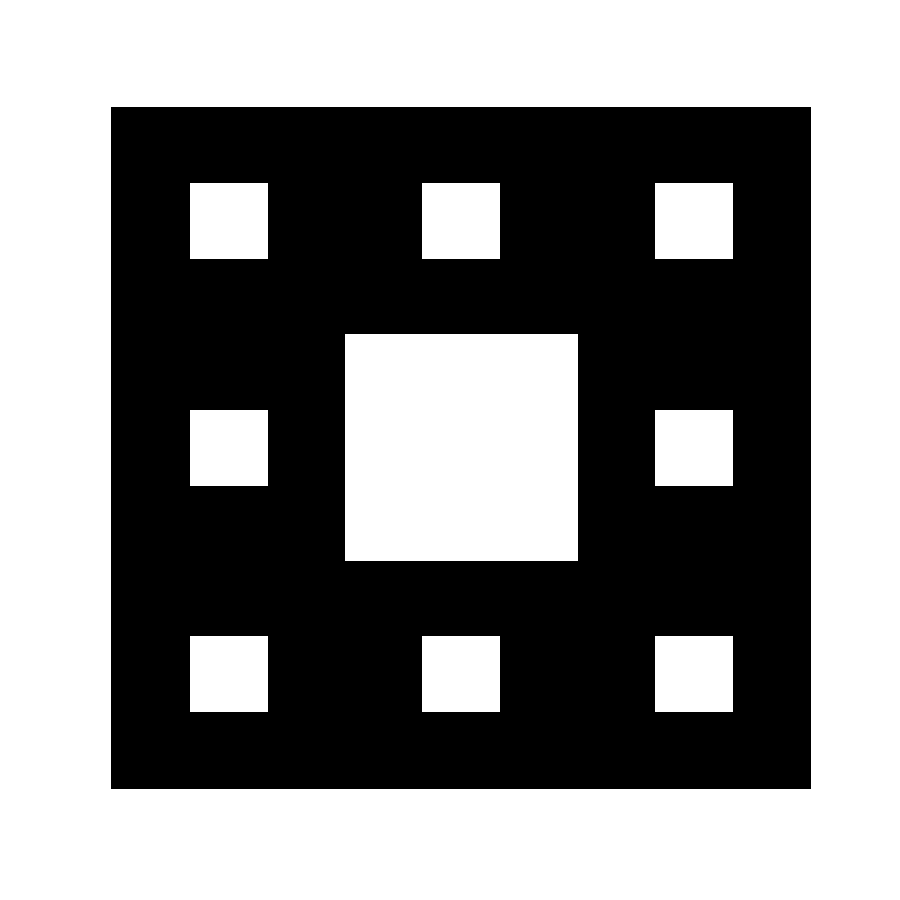
\includegraphics[width=\textwidth]{Imagenes/Fractal/sierpinski_carpet_3.pdf}
     \end{subfigure}\hspace*{-0.9em}
     \begin{subfigure}[b!]{0.27 \textwidth}
         \caption{}
         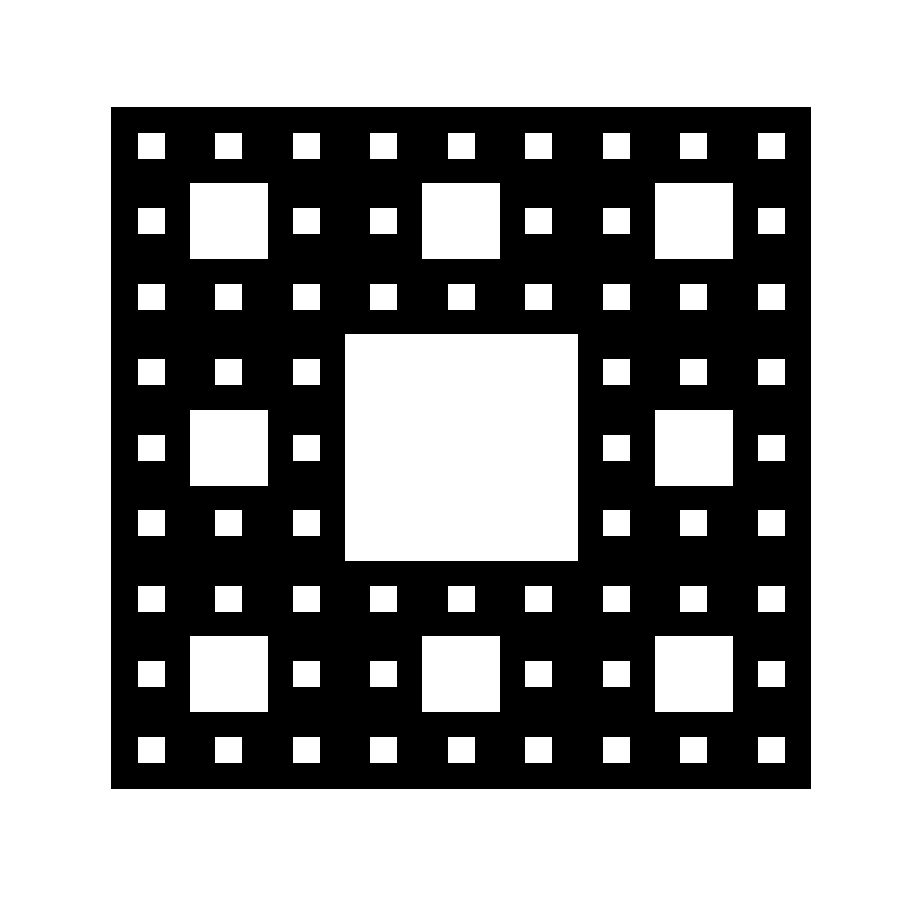
\includegraphics[width=\textwidth]{Imagenes/Fractal/sierpinski_carpet_4.pdf}
     \end{subfigure}
        \caption{Procedimiento para generar una red o alfombra de Sierpinski, conforme aumentan las iteraciones, \textbf{(a)} $n=0$, \textbf{(b)} $n=1$, \textbf{(c)} $n=2$,\textbf{(d)} $n=3$.}
        \label{fig:Fractals}
\end{figure}

Hemos observado que las propiedades electrónicas de los materiales que estudiamos depende casi totalmente de las propiedades geométricas que lo definen. La relaciones y la separación entre los estados de borde y de bulto, permiten construir estados de polarización así como hacer un seguimiento del bombeo de las cargas en parámetros cíclicos. Pero, que pasaría si las geometrías de los materiales, tienen mas de un borde o la idea de la relación cuerpo-borde o área y perímetro se pierden? 

Una de las geometrías mas interesantes que cumplen estas características son las fractales, construcciones geométricas que se basan en la realización iterativa y poseen propiedades como la dimensión no entera, y la autosemejanza. Para los fines de este trabajo nos concentraremos en la alfombra de Sierpinski, el cual es un fractal descrito por el matemático polaco Waclaw Sierpinski en 1916. Se construye dividiendo un cuadrado en otros nueve de lado 1/3 del original y eliminando el cuadrado que ocupa la posición central, repitiendo este proceso en cada uno de los cuadrados que
quedan, indefinidamente.

En cada iteración el numero de huecos cuadrados va aumentando de la siguiente manera (fig \ref{fig:Fractals}):
\begin{equation}
    1,\; 8, \; 8^2,\;\dots\; 8^n
\end{equation}
respectivamente, cada lado del cuadrado escala como un tercio del anterior:
\begin{equation}
    1,\; \frac{1}{3}, \; \left( \frac{1}{3} \right)^2,\;\dots\; \left( \frac{1}{3} \right)^n
\end{equation}
como resultado se obtiene así un objeto geométrico “hueco” de área nula pero con perímetro infinito. Al calcular su dimensión obtenemos:

\begin{equation}
    D = \frac{log N(r)}{log 1/r} = \frac{log 8^n}{log 3^n} = 1.8927
\end{equation}

Donde $N(r)$ es el numero de figuras que se generan por iteración y $r$ es la relación de escala de cada lado por cada iteración.

Los fractales considerados en este trabajo están definidos en un numero finito de iteraciones, además que en la construcción, como se vera en el próximo capitulo, el tamaño de las figuras que conforman el fractal crecen como múltiplos de la celda unitaria, por lo cual no hay una dilución del área solo existe respecto al tamaño final, esto implica que en este trabajo que los fractales considerados en este trabajo sean fractales aproximados.



%
% Descripción del proyecto
%

\chapter{Descripción del proyecto}

%\comA{Los aislantes topológicos pueden subclasificarse por la localización en la frontera de los estados en el gap. Las subclasificación se llama de orden superior y corresponde. Este trabajo esta inspirado en el trabajo publicado por Benalcazar at. all, en el articulo ''Quantized electric multipole insulators'' . La idea central es extender el modelo de SSH a un modelo 2-dimensional de forma cuadrada y otro en una forma de alfombra de Sierpinski, y así poder obtener HOTIs que tengan estados con densidades de probabilidad concentradas principalmente en las esquinas de la geometría. La tesis se enmarca en extender la aparición de hoti a redes fractales...
%}

Los aislantes topológicos están definidos por su relación bulto-frontera. Si un sistema de dimensión $d$ presenta estados con gap en el bulto y además presenta estados robustos ante perturbaciones sin gap en la frontera, se dice que este sistema es un aislante topológico. Sin embargo esta clasificación fue enriquecida con una subclasificación introducida por Benalcazar at. all \cite{Benalcazar2017} debido a sistemas que presentan estados sin gap en las aristas y los vértices, a esta subclasificación se le conoce como aislantes topológicos de orden superior (HOTI). Un aislante topológico de orden $n$-ésimo tiene estados protegidos sin gap en una frontera del sistema de codimensión $n$ \cite{schindler2018higher}.
Esta tesis se enfoca en extender la aparición de HOTI en redes fractales con dimensión de Housdorff fraccional, donde la relación de bulto y fronteras se desdibuja.  Esto se logró tomando el modelo utilizado por Benalcazar at. all en una red cuadrada y aplicarlo una red de Sierpinski.

    \section{Objetivo general}
    
    El objetivo de la tesis es extender la clasificación de aislantes topológicos de orden superior a redes de dimensión fractal, como lo es una red Sierpisnki cuadrada. También hacer un estudio que compare el comportamiento de las propiedades electrónicas de estados topológicos y no topológicos y su transición entre las redes cuadradas y redes de Sierpinski con los modelo Benalcazel, Bernevig, Taylor (BBT).

Particularmente, en los sistemas de geometría 2-dimensional se ha observados que al tener una transición adiabática de fase topológica a trivial y de trivial a topológica puede generar un bombeo de carga (Thouless pump \cite{benalcazar2020higher}) generado por el el flujo de los centros de Wannier. Debido a esto centramos nuestra atención en determinar si los HOTIs fractales también puede presentar bombeo de carga utilizando un modelos 2-dimensional inspirado en el modelo Rice-Mele.
    
    \section{Objetivo particular}
    \begin{itemize}
        \item Observar estados topológicos de orden superior en la red de Sierpinski y una red cristalina cuadrada.
        \item Caracterizar el cambio de la densidad (electrónica) de probabilidad en una transición de fase topológica a trivial. 
        \item Generar un espacio fase de la corriente como función de los parámetros $\gamma, \lambda$, con el fin de determinar cuándo el flujo de densidad de corriente será máximo.
        \item Determinar para que variación de parámetros existe bombeo de densidad de probabilidad en la red cristalina cuadrada y fractal.
    \end{itemize}
    
\section{Detalles de la implementación}
    

\subsection{SSH 2D en una Red Cuadrada y en una alfombra de Sierpinski}\label{Modelo_SSH_squara_and_Fractal}

    Notemos que la idea del modelo de SSH se puede extender de manera sencilla a algunos casos en 2 dimensiones, como lo es para una red cristalina cuadrada. Supongamos que tenemos una red cristalina cuadrada, con 16 sitios y 4 subredes o celdas unitarias, cada una compuesta por 4 sitios como se ve en la fig( agregar fig), con $\gamma$ y $\lambda$ los parámetros de salto, intracelda e intercelda, respectivamente. Siguiendo el modelo de SSH el hamitoniano de este sistema estará dado la matriz de conexión definida como: 
    
    
    \begin{figure}[h!]
     \centering
    \captionsetup[sub]{font=small}

     \begin{subfigure}[b!]{0.27 \textwidth}
         \caption{}
         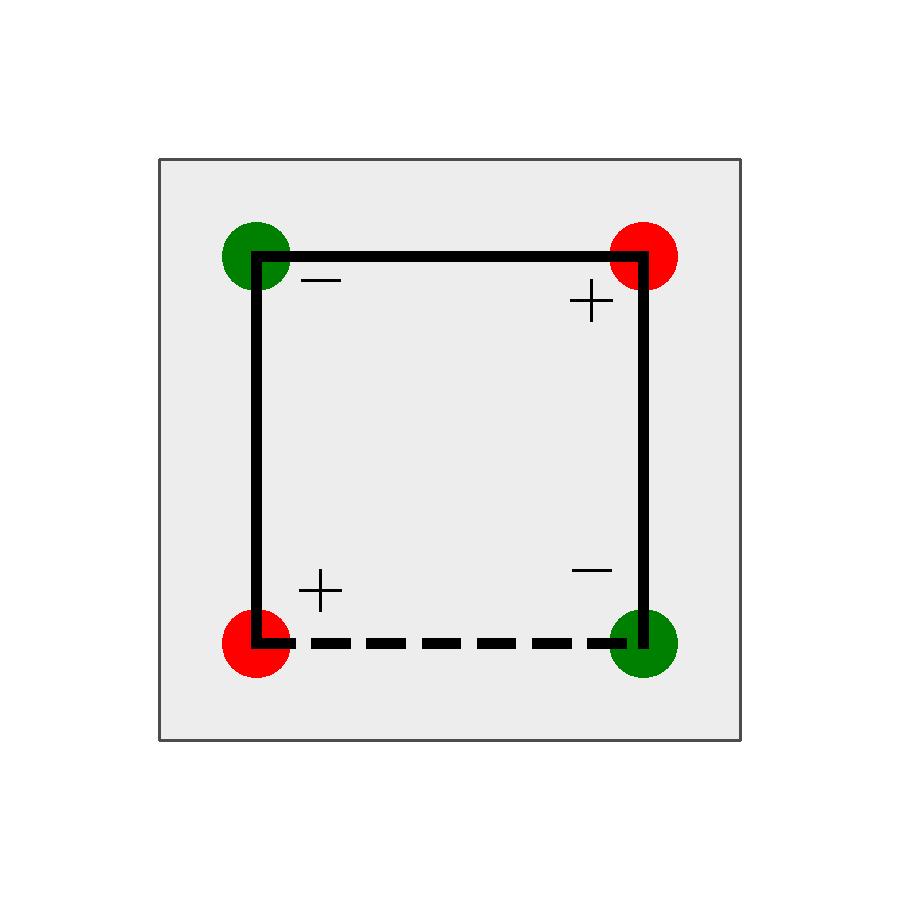
\includegraphics[width=\textwidth]{Imagenes/Models/unitary_cell.pdf}
         \label{}
     \end{subfigure}\hspace*{-0.5em}
     \begin{subfigure}[b!]{0.27 \textwidth}
         \caption{}
         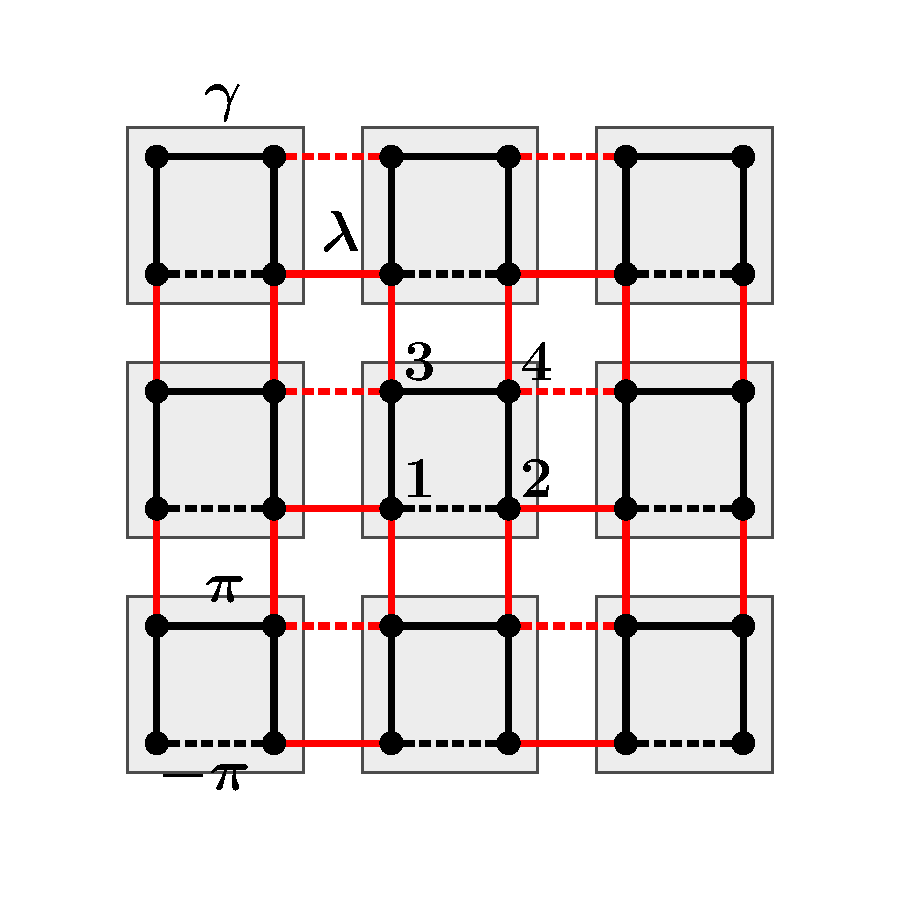
\includegraphics[width=\textwidth]{Imagenes/Models/square_hoti_model6.pdf}
         \label{}
     \end{subfigure}\hspace*{-0.3em}
     \begin{subfigure}[b!]{0.27 \textwidth}
         \caption{}
         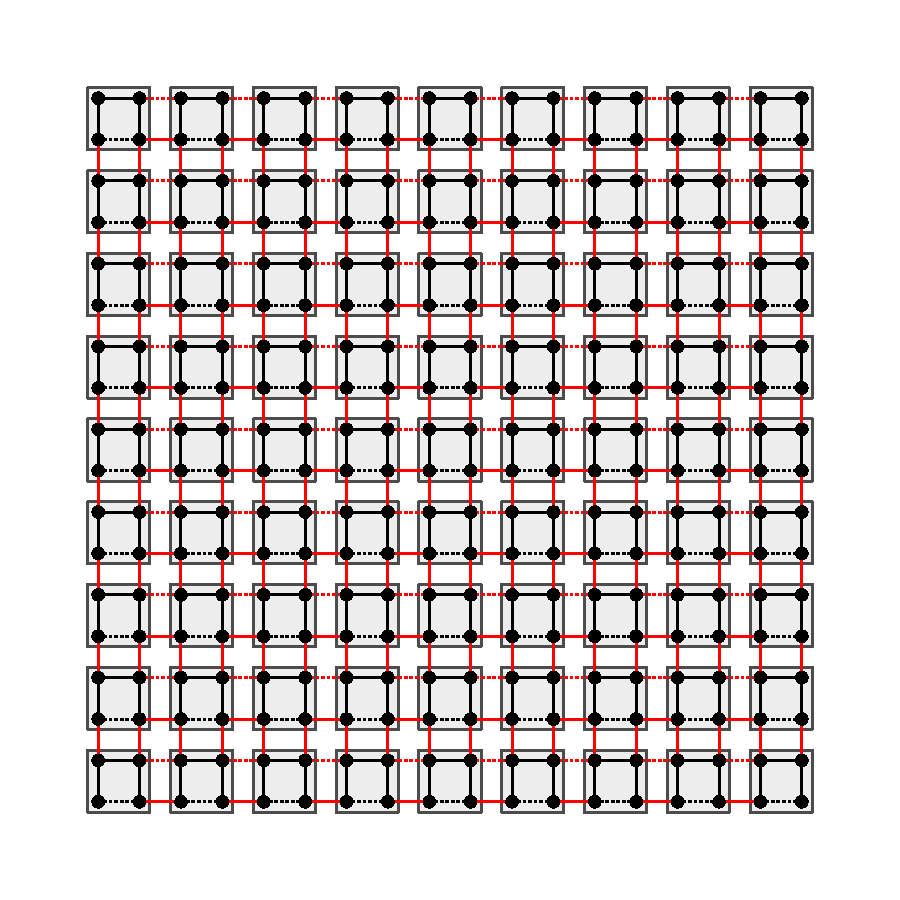
\includegraphics[width=\textwidth]{Imagenes/Models/square_hoti_model.pdf}
         \label{}
     \end{subfigure}\hspace*{-0.3em}
     \begin{subfigure}[b!]{0.27 \textwidth}
         \caption{}
         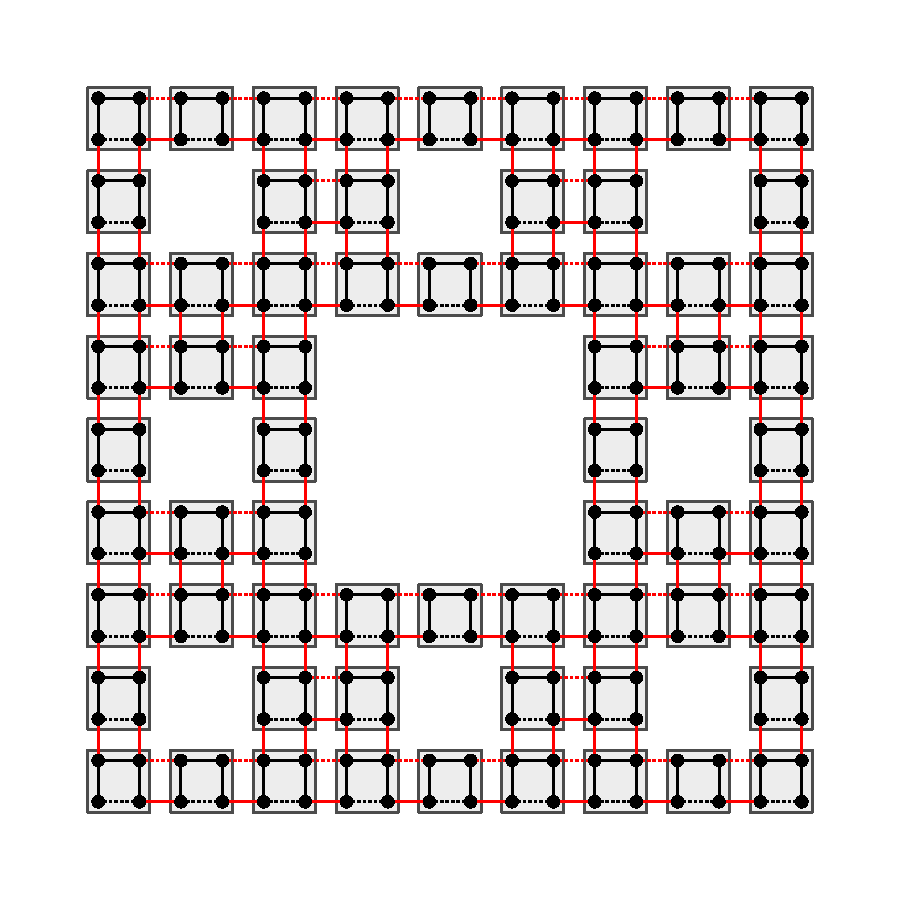
\includegraphics[width=\textwidth]{Imagenes/Models/fractal_hoti_model.pdf}
         \label{}
     \end{subfigure}
     
        \caption{Three simple graphs}
        \label{fig:three graphs}
\end{figure}
    
    \begin{equation} 
         H = 
     \begin{pmatrix}
        0 & \gamma & \gamma & 0 & 0 & 0 & 0 & 0 & 0 & 0 & 0 & 0 & 0 & 0 & 0 & 0 & \\
        \gamma & 0 & 0 & \gamma &\lambda & 0 & 0 & 0 & 0 & 0 & 0 & 0 & 0 & 0 & 0 & 0  \\
        \gamma & 0 & 0 & \gamma & 0 & 0 & 0 & 0 & \lambda & 0 & 0 & 0 & 0 & 0 & 0 & 0 \\
        0 & \gamma & \gamma & 0 & 0 & 0 & \lambda & 0 & 0 & \lambda & 0 & 0 & 0 & 0 & 0 & 0 \\
        0 & \lambda & 0 & 0 & 0 & \gamma & \gamma & 0 & 0 & 0 & 0 & 0 & 0 & 0 & 0 & 0 \\
        0 & 0 & 0 & 0 & \gamma & 0 & 0 & \gamma & 0 & 0 & 0 & 0 & 0 & 0 & 0 & 0 \\
        0 & 0 & 0 & \lambda & \gamma & 0 & 0 & \gamma & 0 & 0 & 0 & 0 & \lambda & 0 & 0 & 0 \\
        0 & 0 & 0 & 0 & 0 & \gamma & \gamma & 0 & 0 & 0 & 0 & 0 & 0 &\lambda & 0 & 0 \\
        
        0 & 0 & \lambda & 0 & 0 & 0 & 0 & 0 & 0 & \gamma & \gamma & 0 & 0 &0 & 0 & 0 \\
        0 & 0 & 0 & \lambda & 0 & 0 & 0 & 0 & \gamma & 0 & 0 & \gamma  & \lambda & 0 & 0 & 0 \\
        0 & 0 & 0 & 0 & 0 & 0 & 0 & 0 & \gamma & 0 & 0 & \gamma  &0 & 0 & 0 & 0 \\
        0 & 0 & 0 & 0 & 0 & 0 & 0 & 0 & 0 & \gamma & \gamma & 0 & 0 &0 & \lambda  & 0 \\
        
        0 & 0 & 0 & 0 & 0 & 0 & \lambda & 0 & 0 & \lambda & 0 & 0 & 0 & \gamma & \gamma & 0 \\
        0 & 0 & 0 & 0 & 0 & 0 & 0 & \lambda & 0 & 0 & 0 & 0 & \gamma & 0 & 0 & \gamma  \\
        0 & 0 & 0 & 0 & 0 & 0 & 0 & 0 & 0 & 0 & 0 & \lambda & \gamma & 0 & 0 & \gamma \\
        0 & 0 & 0 & 0 & 0 & 0 & 0 & 0 & 0 & 0 & 0 & 0 & 0 & \gamma & \gamma & 0 \\
        
    \end{pmatrix}
    \end{equation}
    
     
    Como podemos notar, las matrices que describen a estos sistemas son matrices de conexión por lo tanto es una matriz simétrica, de igual forma que en el caso uni-dimensional, es posible suponer condiciones periódicas a las frontera y obtener la matriz expresada en el espacio de momentos:
    
    \begin{equation}
    H =      
     \begin{pmatrix}
            0 & \gamma + \lambda e^{-ik_x} & 0 &  \gamma + \lambda e^{-ik_y} \\
             \gamma + \lambda e^{ik_x} & 0 &  \gamma + \lambda e^{-ik_y} & 0  \\
            0 & \gamma + \lambda e^{ik_y} & 0 &  \gamma + \lambda e^{ik_x} \\
             \gamma + \lambda e^{ik_y} & 0 &  \gamma + \lambda e^{-ik_x} & 0  \\
     \end{pmatrix} 
    \end{equation}

Donde $k_x$ y $k_y$ son las proyecciones del vector $\mathbf{k}$ de momentos sobre las direcciones $\mathbf{x}$ y $\mathbf{y}$, es decir, $\mathbf{k} = (k_x, k_y)$  


Ahora ¿Cómo implementamos la idea del HOTI cuadrado con el modelo de SSH 2D en nuestra en una alfombra de Sierpinski? Una de las primeras cosas es notar como es el proceso iterativo de la construcción de una alfombra de Sierpinski, este proceso se describe la sección (poner sección), para esta construcción se comenzó con un cuadrado inicial compuesto por 9 celdas unitarias y 36 sitos, a este cuadrado se le extrae la celda unitaria del centro, esta idea sea itera N veces obteniendo la red fractal que esperamos (figura de iteraciones), a diferencia del escalamiento que se observa en la construcción común de un fractal, para mantener las celdas con el mismo tamaño es necesario hacer el sistema cada vez mas grande. 
El hamitoniano que describe a este sistema estará dado por la matriz de conexión (figura matriz de conexión), sin embargo, dado que este sistema no tiene simetría traslación sobre la celda unitaria no es posible tener un hamiltoniano de Bloch que nos permita encontrar la solución en el espacio reciproco y así estudiar las propiedades electrónicas de las que nos podría proveer la teoría de bandas.

Debido a las limitantes computacionales el estudio de este sistema se fijo en la segunda  iteración ($N=2$) en la construcción del la alfombra de Sierpinski con (tantos) sitios y el modelo de la red cuadrada se limito a un cuadrado compuesto por 81 celdas y 324 sitios (figura matriz de conexión). 

\subsection{Centros de Wannier en el espacio real}

Uno de los problemas principales al momento de calcular las cantidades topológicas como la fase de Berry en estructuras geométricas como los fractales es la falta de periodicidad en el sistema, lo cual no permite tener un hamiltoniano de Bloch que nos permita usar las expresiones (agregar ecuaciones de la fase de Berry continua). Afortunadamente existen otras formas de construir este invariante sin necesidad de usar funciones de Bloch, y es a través del operador de posición, este nos permite extraer los estados sobre los cuales sumaremos las contribuciones de la fase, esta forma es numéricamente estable y además es invariante de norma (referencia A short Course).

Consideremos una cadena con $N$ elementos y largo $L$ con condiciones periódicas a la frontera, su operador de posición unitario estará dado por:
\begin{equation}
    \hat{X} = e^{i\delta_k \hat{x}}
\end{equation}
Con $\delta_k = L/N$. El valor esperado de la posición asociado al estado $\ket{\psi}$ se calculara como:
\begin{equation}
    \expectv{\hat{X}} = \frac{N}{2\pi} \; \text{arg} \; \sandwich{\psi}{\hat{X}}{\psi}
\end{equation}
Para poder calcular los centros de Wannier restringiremos el operador de posición únicamente a las bandas llenas:
\begin{equation}
    \hat{X}_P = \hat{P} \hat{X} \hat{P}
\end{equation}

Con $\hat{P} = \sum_{m = 1}^{N_{occ}} \sum_{k} \ket{\psi_{m,k}} \bra{\psi_{m,k}}$, para simplificar el operador $\hat{X}_P$  consideremos:
\begin{align}
    \sandwich{\psi_{m',k'}}{\hat{X}}{\psi_{m,k}} &= \frac{1}{N} \sum_{m'} e^{-im'k'} \bra{u_{m'}^{k'}}   \sum_{m} e^{im\delta_k} e^{imk}  \ket{u_{m}^{k}} \nonumber \\
    &=  \frac{1}{N} \braket{u_{m}^{k'}}{u_{m}^{k}} \sum_{m} e^{-im(k + \delta_k - k')} \nonumber \\
    &= \delta_{k + \delta_k, k'} \frac{1}{N} \braket{u_{m}^{k + \delta_k}}{u_{m}^{k}}  
\end{align}
Donde $\delta_{k + \delta_k, k'}$ sera $1$ cuando $k' = \delta_k + k$ y $0$ en cualquier otro caso, usando esto obtenemos:
\begin{align}
    \hat{X}_P &=  \sum_{m,m'=1}^{N_{occ}} \sum_{k,k'} \ket{\psi_{m',k'}} \bra{\psi_{m',k'}} \hat{X} \ket{\psi_{m,k}} \bra{\psi_{m,k}} \nonumber \\
    &= \sum_{m,n = 1}^{N_{occ}} \sum_{k} \ket{\psi_{n,k + \delta_k}} \braket{u_{n}^{k +\delta_k}}{u_{m}^{k}} \bra{\psi_{m,k}}
\end{align}
Podemos resolver la $N$-sima potencia de este sistema como un sistema de eigenvalores sobre el $m$-simo sitio ocupado:
\begin{equation}
    (\hat{X}_P)^N \ket{\nu^m} =  W \ket{\nu^m}
\end{equation}
Al termino de la derecha se le conoce como la linea de Wilson sobre un parametro ciclico, donde los elementos de matriz están conformados por las fases de Berry discretas sobre $k$:
\begin{equation}
    W_{i,j} = \delta_{i,j} \braket{u_m^{k+\delta_k}}{u_m^{k}} \braket{u_m^{k}}{u_m^{k-\delta_k}} \dots \braket{u_m^{k +2\pi -\delta_k}}{u_m^{k-2\pi}} 
\end{equation}
Donde $\delta_{i,j}$ es $1$ cuando $i = j+1$ y $0$ en otros casos. Con esto es posible determinar los centros de Wannier que estarán dados por los eigenvalores de la siguiente ecuacion ()

\begin{equation}
    W \ket{\nu^m}=(E^m)^N \ket{\nu^m}
\end{equation}

suponiendo que el Willson loop es un operador unitario, el problema se convierte en un problemas de fases ():
\begin{equation}
    (E^m)^N \ket{\nu^m} = e^{i2\pi\nu^m} \ket{\nu^m}
\end{equation}
Obteniendo como resultado final, la expresión de los centros de wanier asociados a la $m$-sima banda ocupada, en función del operador posición y el operador de proyección:

\begin{equation}
\label{eq:Wannier_center}
    \nu^m = \frac{N}{2\pi} \; \text{arg} \; \hat{X}_P
\end{equation}





\subsection{Bombeo en un red cuadrada y en una alfombra de Sierpinski}


 %\renewcommand{\thesubfigure}{\roman{subfigure}}
\begin{figure}[h!]
     \centering
    \captionsetup[sub]{font=small}
     \begin{minipage}[h!]{1\textwidth}
         \begin{subfigure}[b!]{0.2 \textwidth}
             \caption{$\theta = - \pi$}
             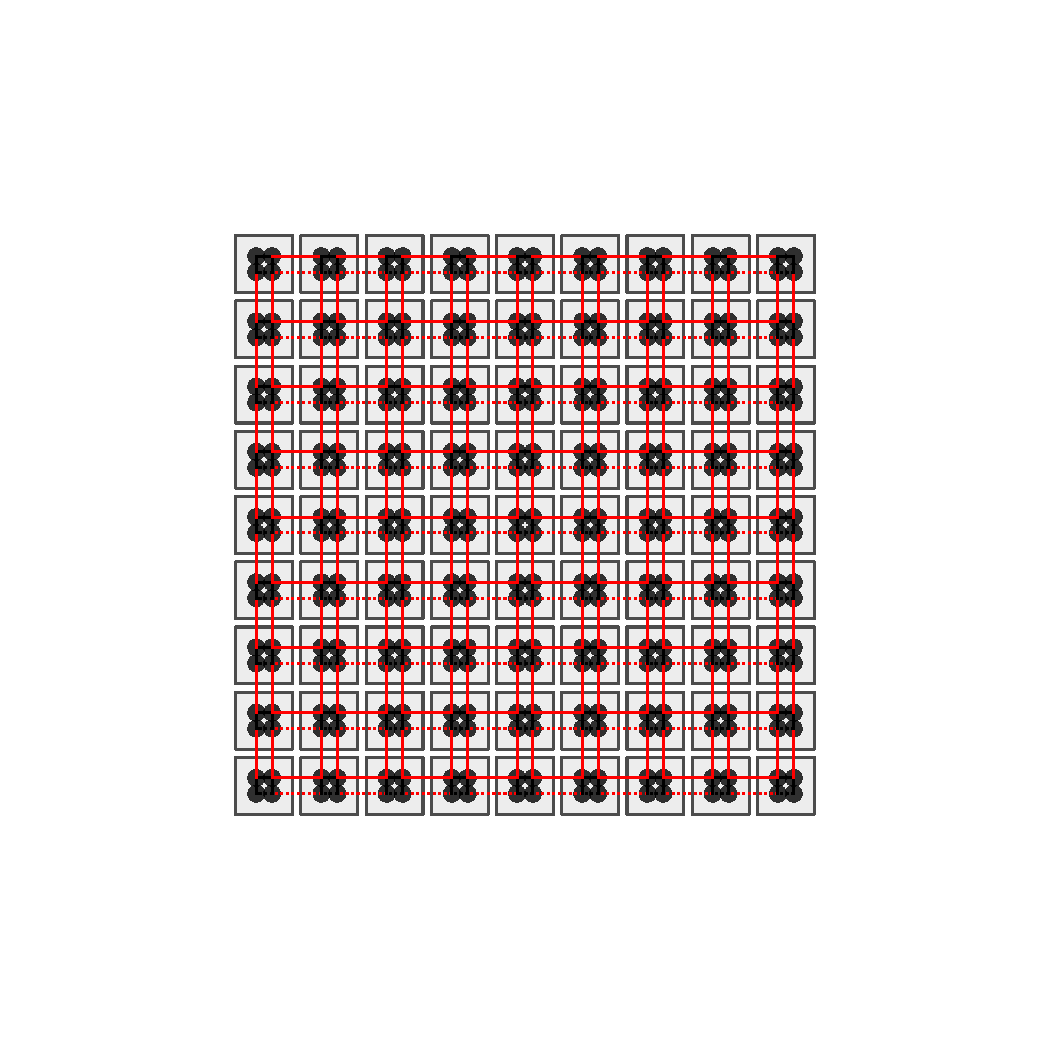
\includegraphics[width=\textwidth]{Imagenes/Models/Model_pump/square_pump_model_xy_0.pdf}
         \end{subfigure}\hspace*{-0.5em}
         \begin{subfigure}[b!]{0.2 \textwidth}
             \caption*{$\theta = -\frac{\pi}{2}$}
             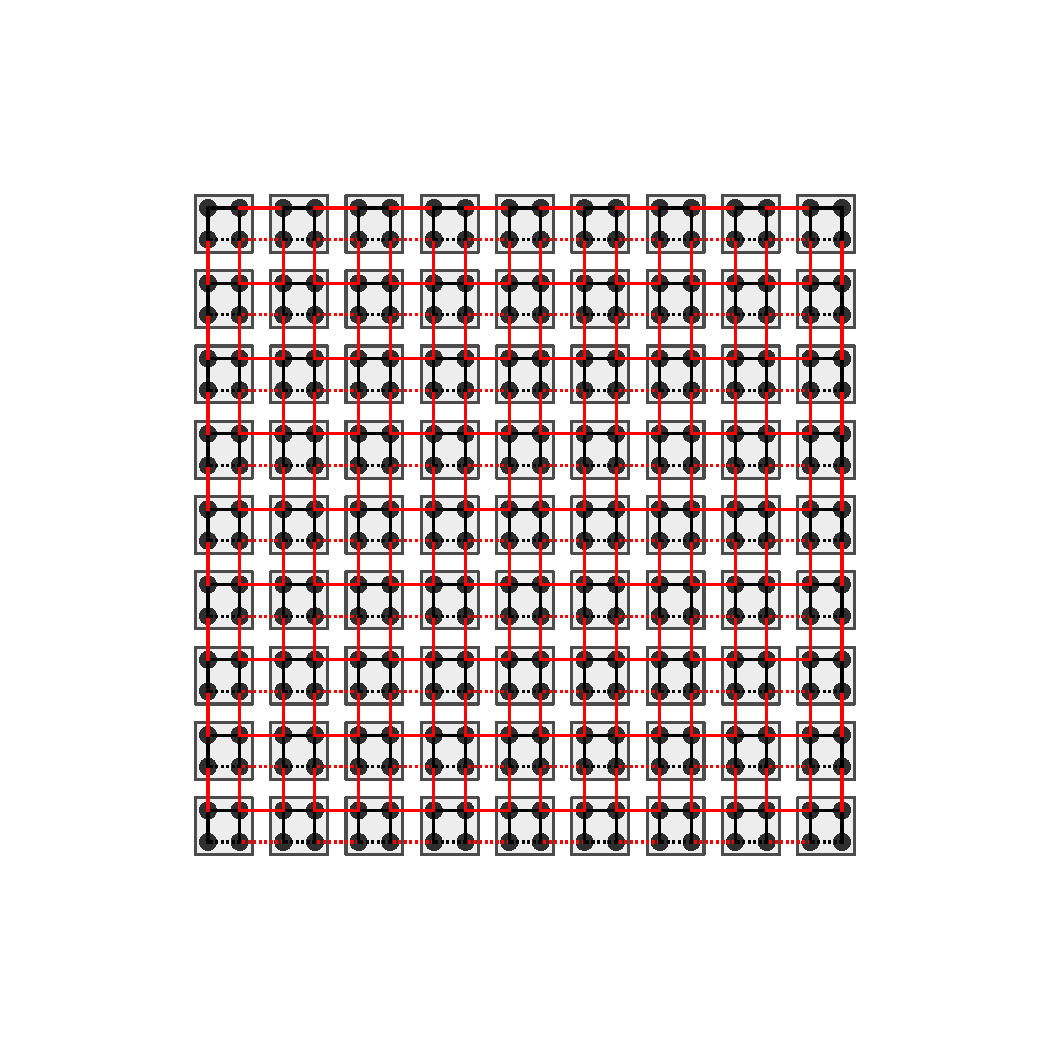
\includegraphics[width=\textwidth]{Imagenes/Models/Model_pump/square_pump_model_xy_5.pdf}
         \end{subfigure}\hspace*{-0.5em}
         \begin{subfigure}[b!]{0.2 \textwidth}
             \caption*{$\theta = 0$}
             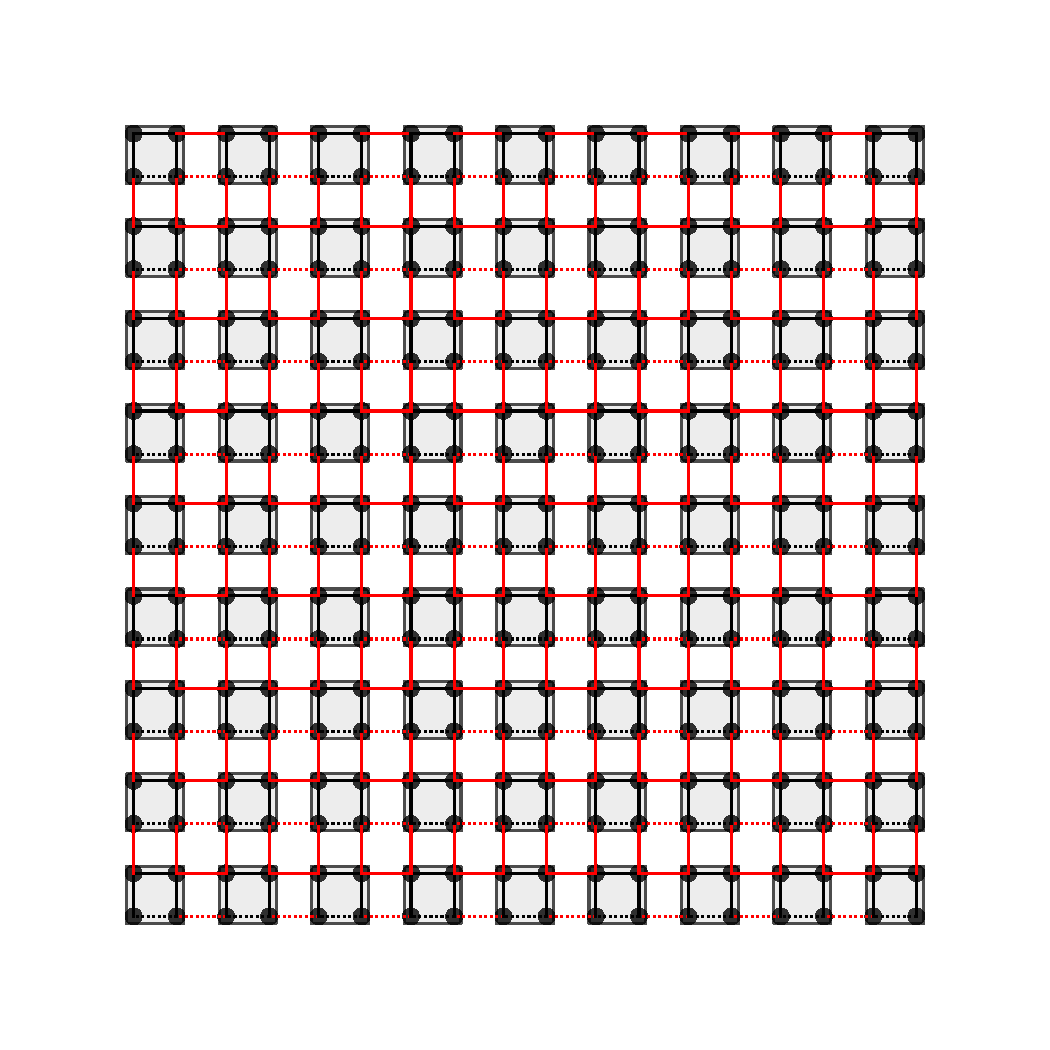
\includegraphics[width=\textwidth]{Imagenes/Models/Model_pump/square_pump_model_xy_8.pdf}
         \end{subfigure}\hspace*{-0.5em}
         \begin{subfigure}[b!]{0.2 \textwidth}
             \caption*{$\theta = \frac{\pi}{2}$}
             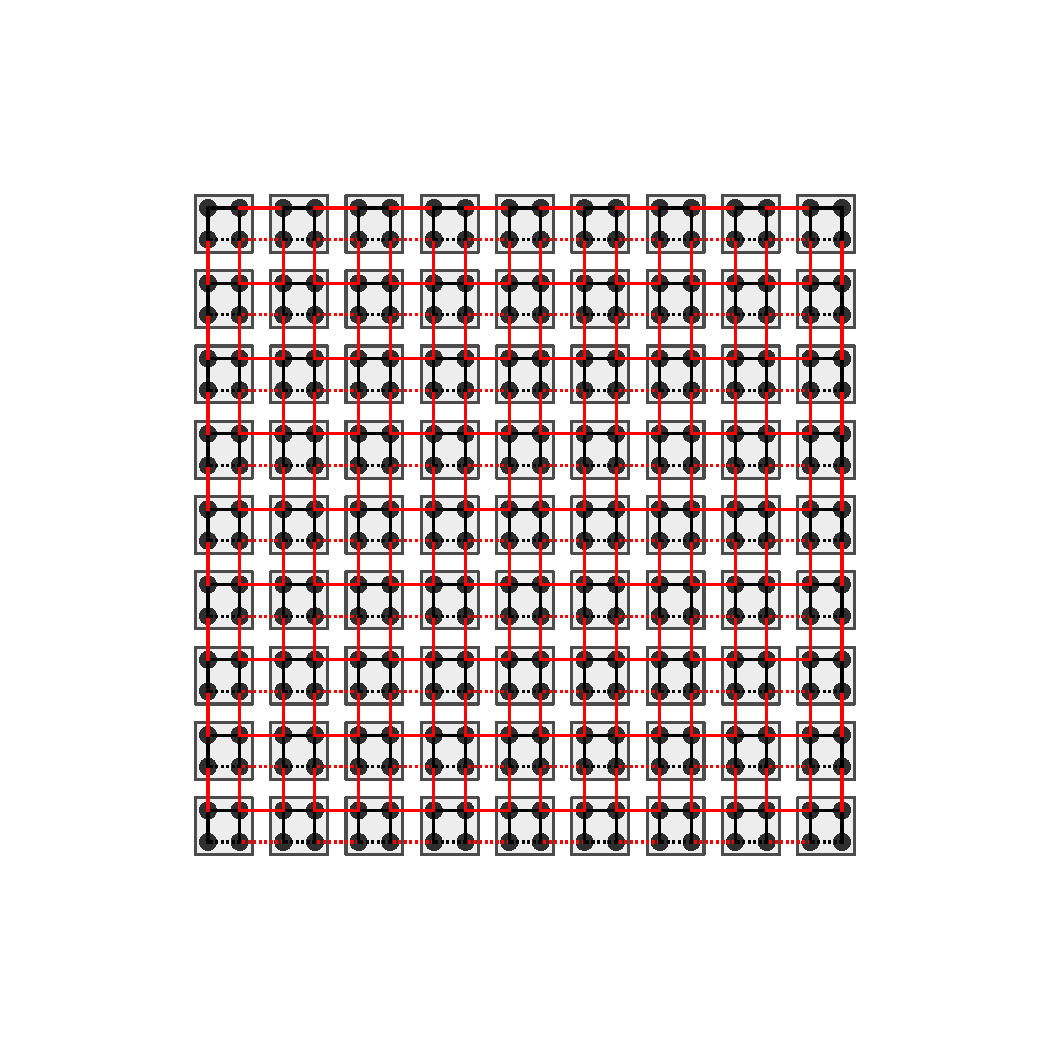
\includegraphics[width=\textwidth]{Imagenes/Models/Model_pump/square_pump_model_xy_11.pdf}
         \end{subfigure}\hspace*{-0.5em}
         \begin{subfigure}[b!]{0.2 \textwidth}
             \caption*{$\theta = \pi$}
             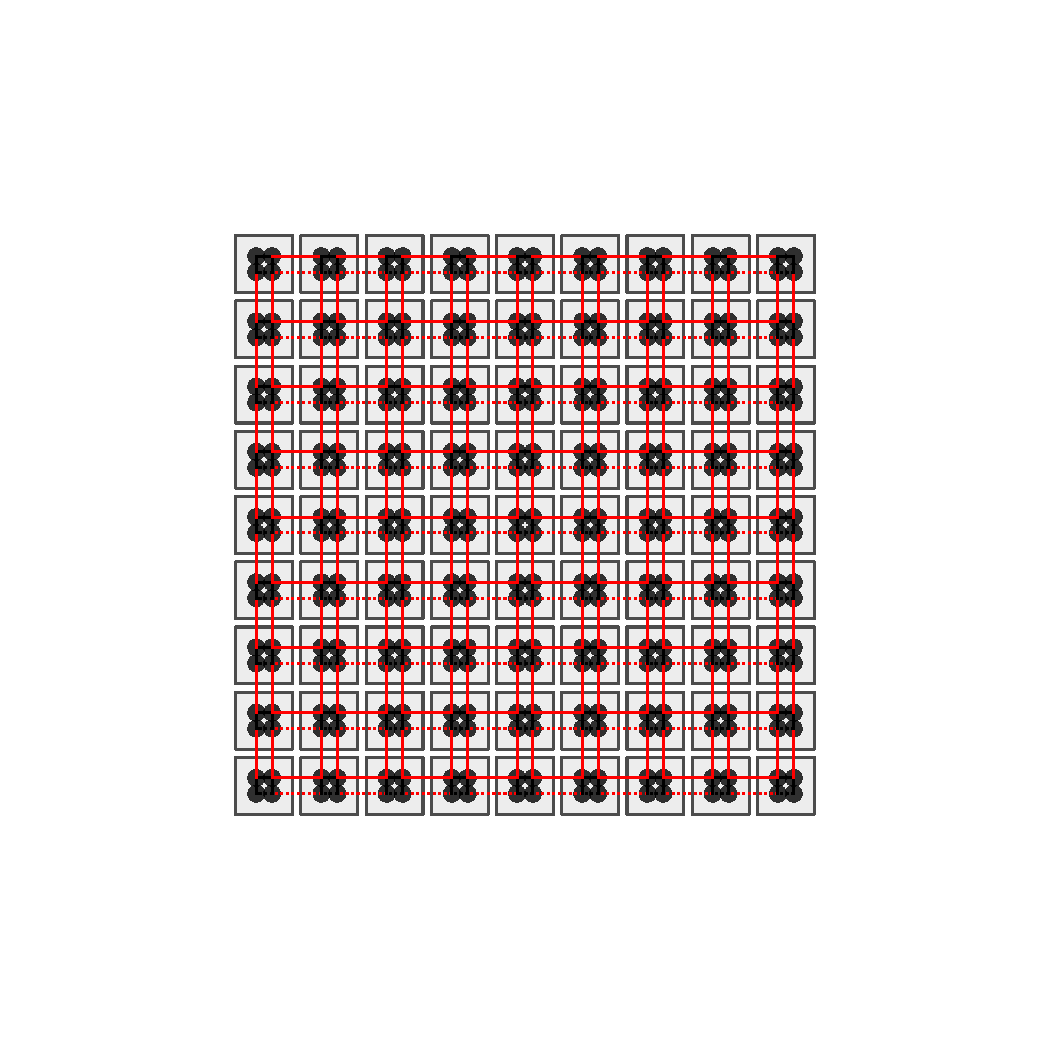
\includegraphics[width=\textwidth]{Imagenes/Models/Model_pump/square_pump_model_xy_16.pdf}
         \end{subfigure}\hspace*{-0.5em}
     \end{minipage}\vspace*{-1em}
     
     
     \begin{minipage}[h!]{1\textwidth}
         \begin{subfigure}[b!]{0.2 \textwidth}
             \caption{}
             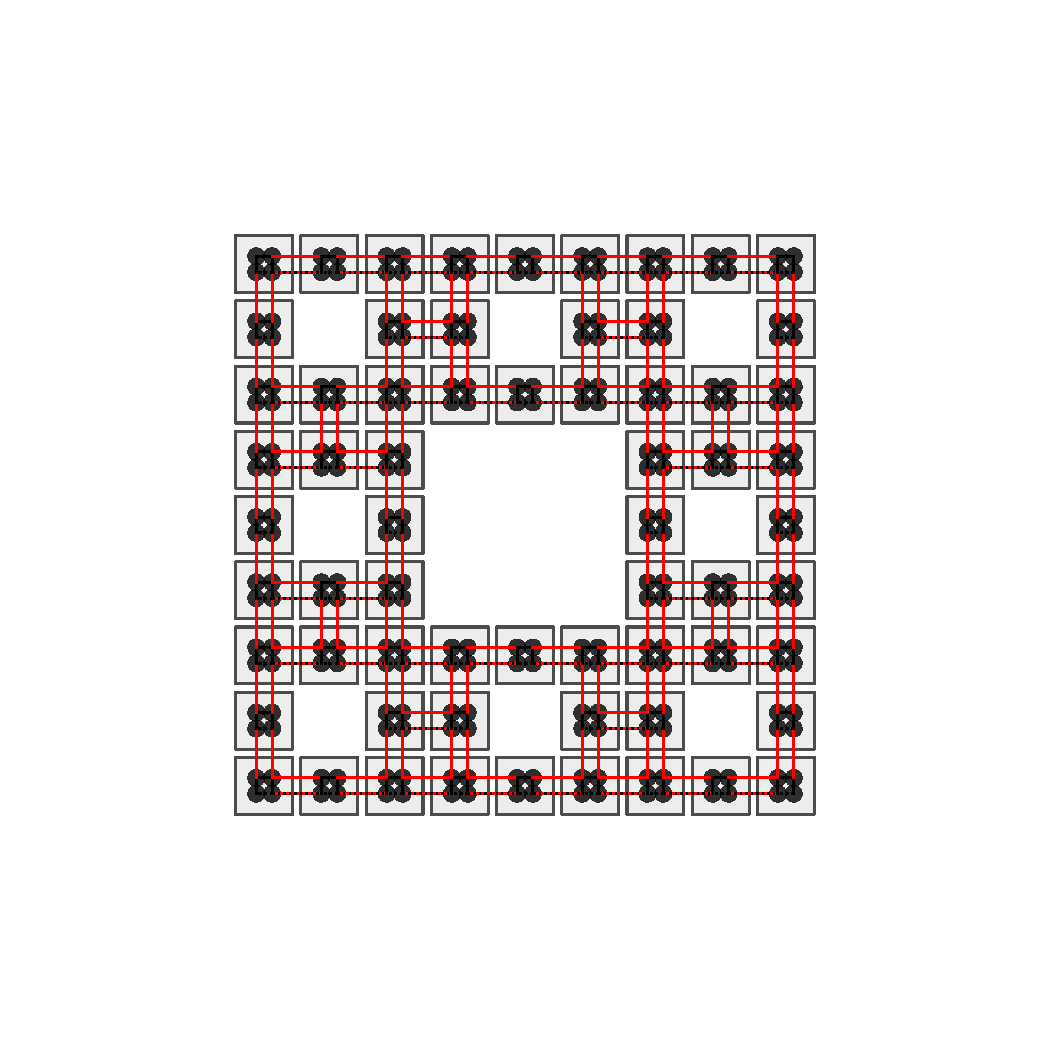
\includegraphics[width=\textwidth]{Imagenes/Models/Model_pump/fractal_pump_model_xy_0.pdf}
         \end{subfigure}\hspace*{-0.5em}
         \begin{subfigure}[b!]{0.2 \textwidth}
             \caption*{}
             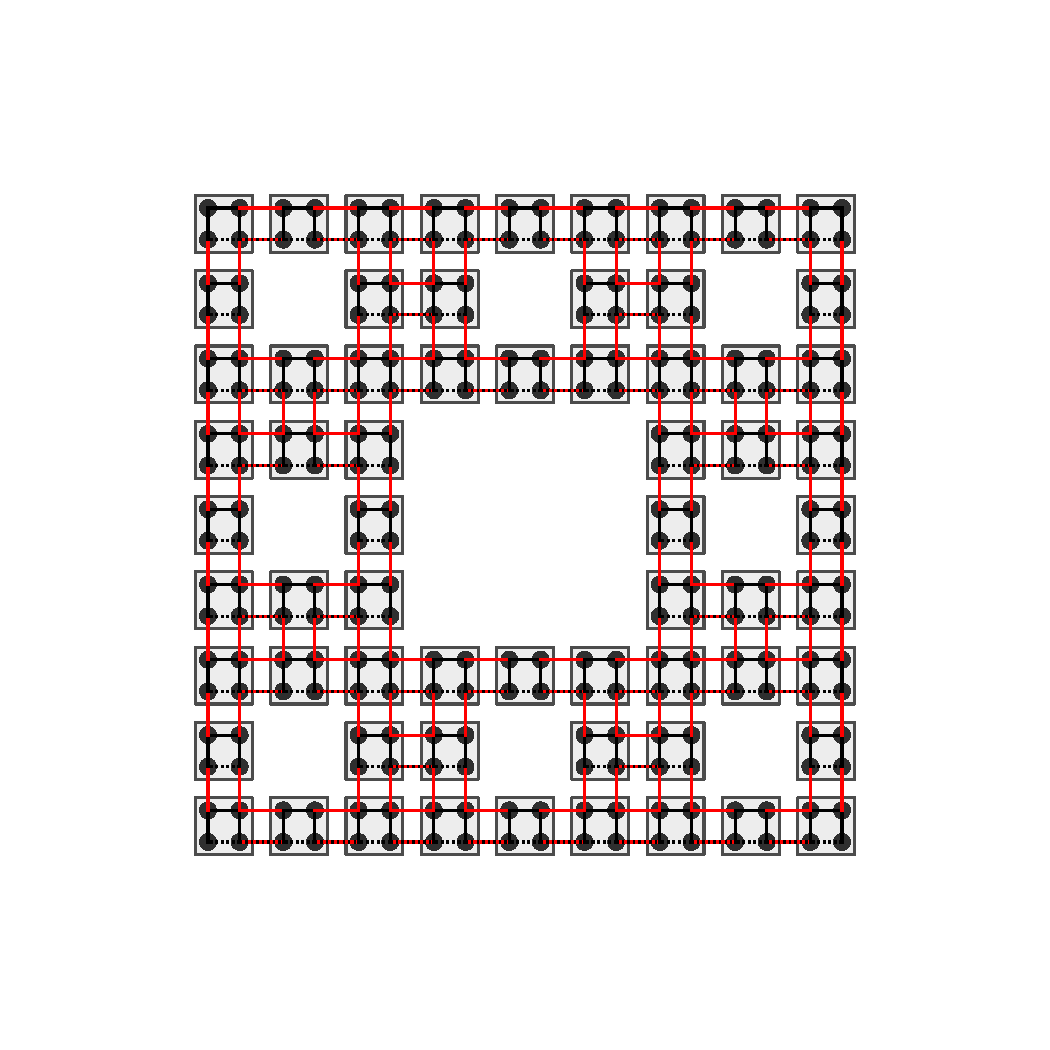
\includegraphics[width=\textwidth]{Imagenes/Models/Model_pump/fractal_pump_model_xy_5.pdf}
         \end{subfigure}\hspace*{-0.5em}
         \begin{subfigure}[b!]{0.2 \textwidth}
             \caption*{}
             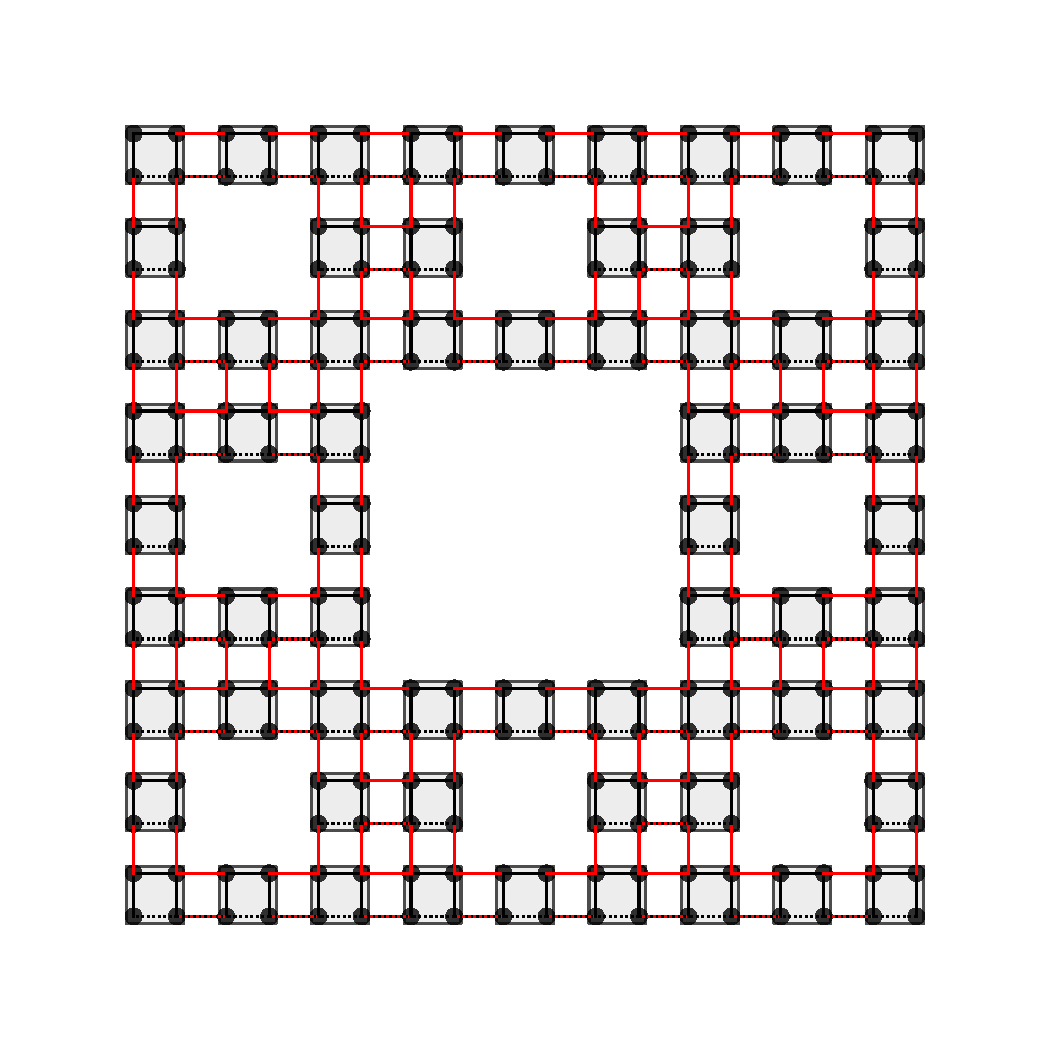
\includegraphics[width=\textwidth]{Imagenes/Models/Model_pump/fractal_pump_model_xy_8.pdf}
         \end{subfigure}\hspace*{-0.5em}
         \begin{subfigure}[b!]{0.2 \textwidth}
             \caption*{}
             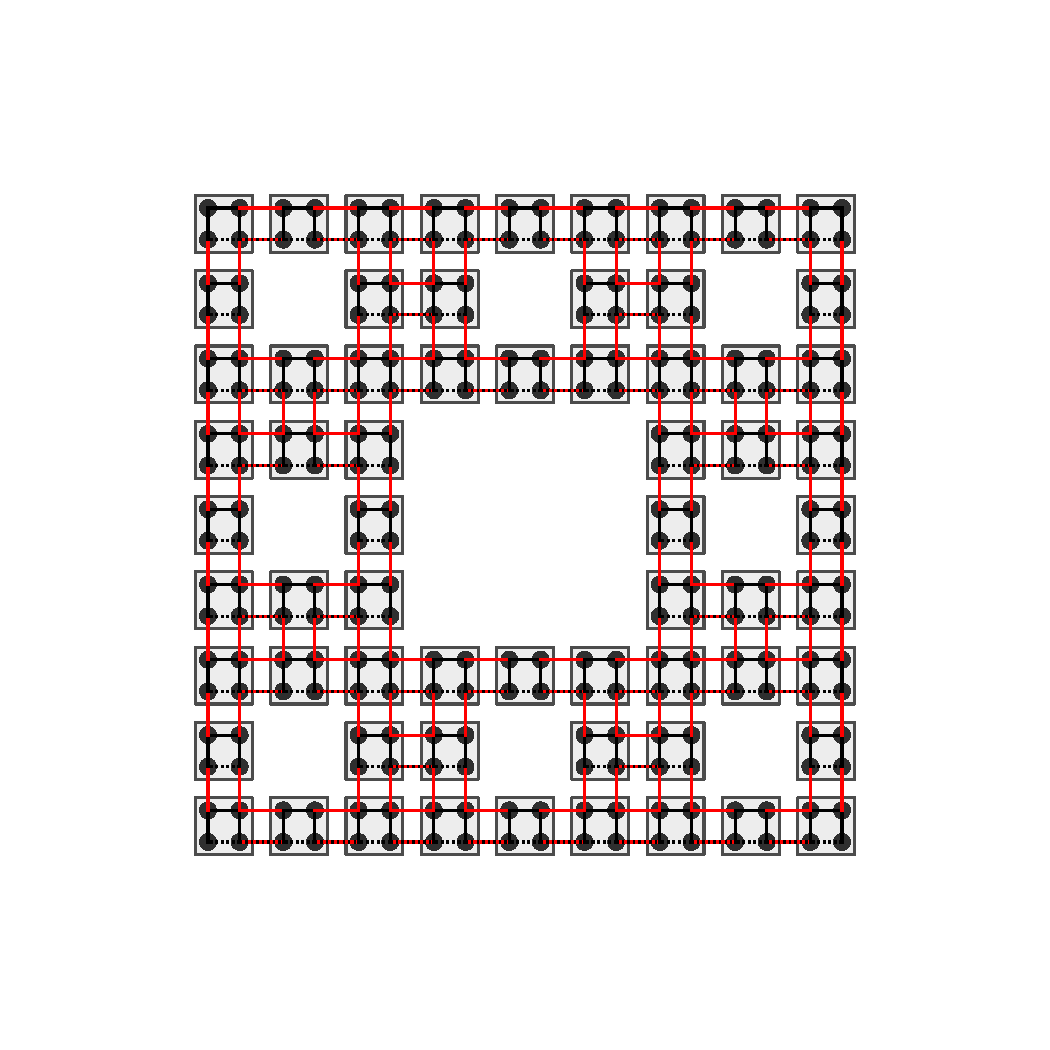
\includegraphics[width=\textwidth]{Imagenes/Models/Model_pump/fractal_pump_model_xy_11.pdf}
         \end{subfigure}\hspace*{-0.5em}
         \begin{subfigure}[b!]{0.2 \textwidth}
             \caption*{}
             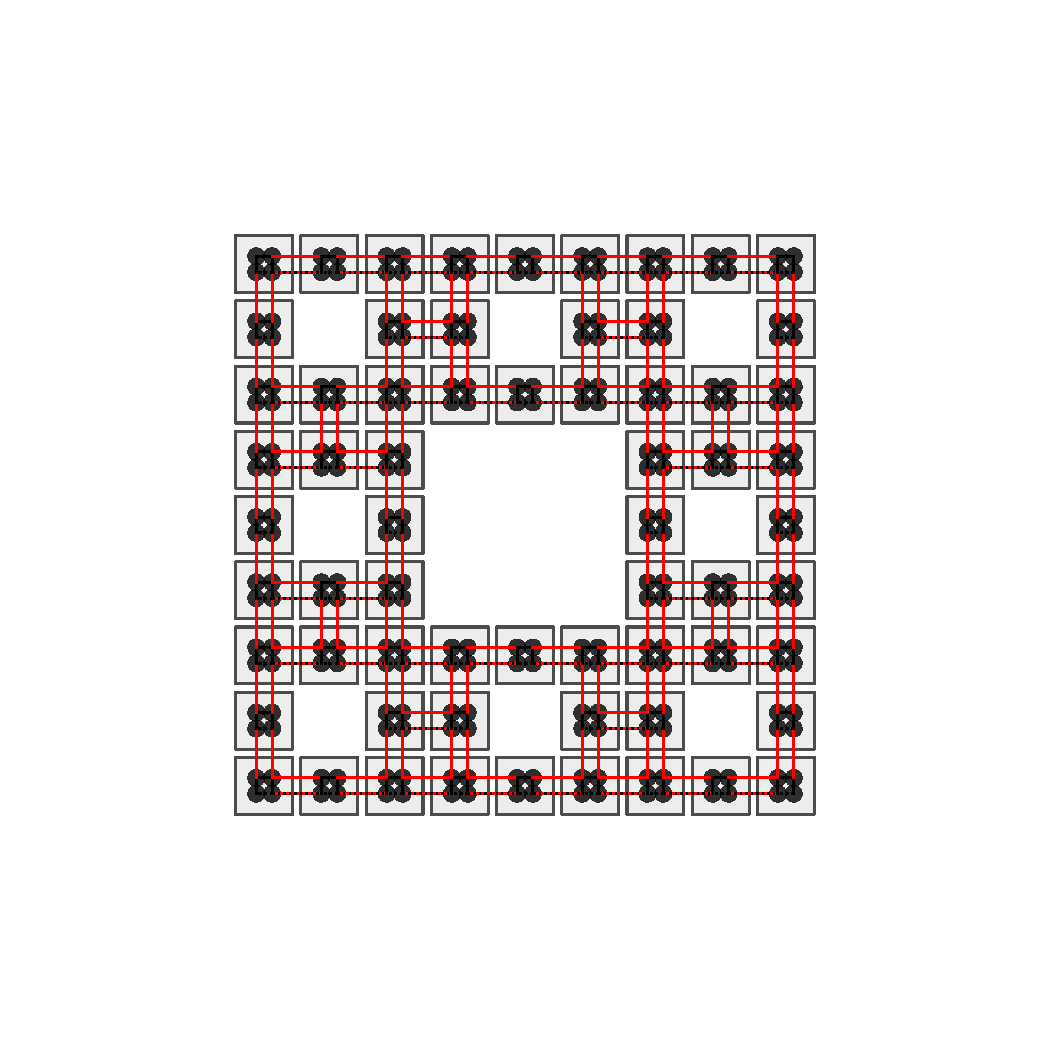
\includegraphics[width=\textwidth]{Imagenes/Models/Model_pump/fractal_pump_model_xy_16.pdf}
         \end{subfigure}\hspace*{-0.5em}
     \end{minipage}\vspace*{-1em}
     
     
     \begin{minipage}[h!]{1.0\textwidth}
         \begin{subfigure}[b!]{0.2 \textwidth}
             \caption{}
             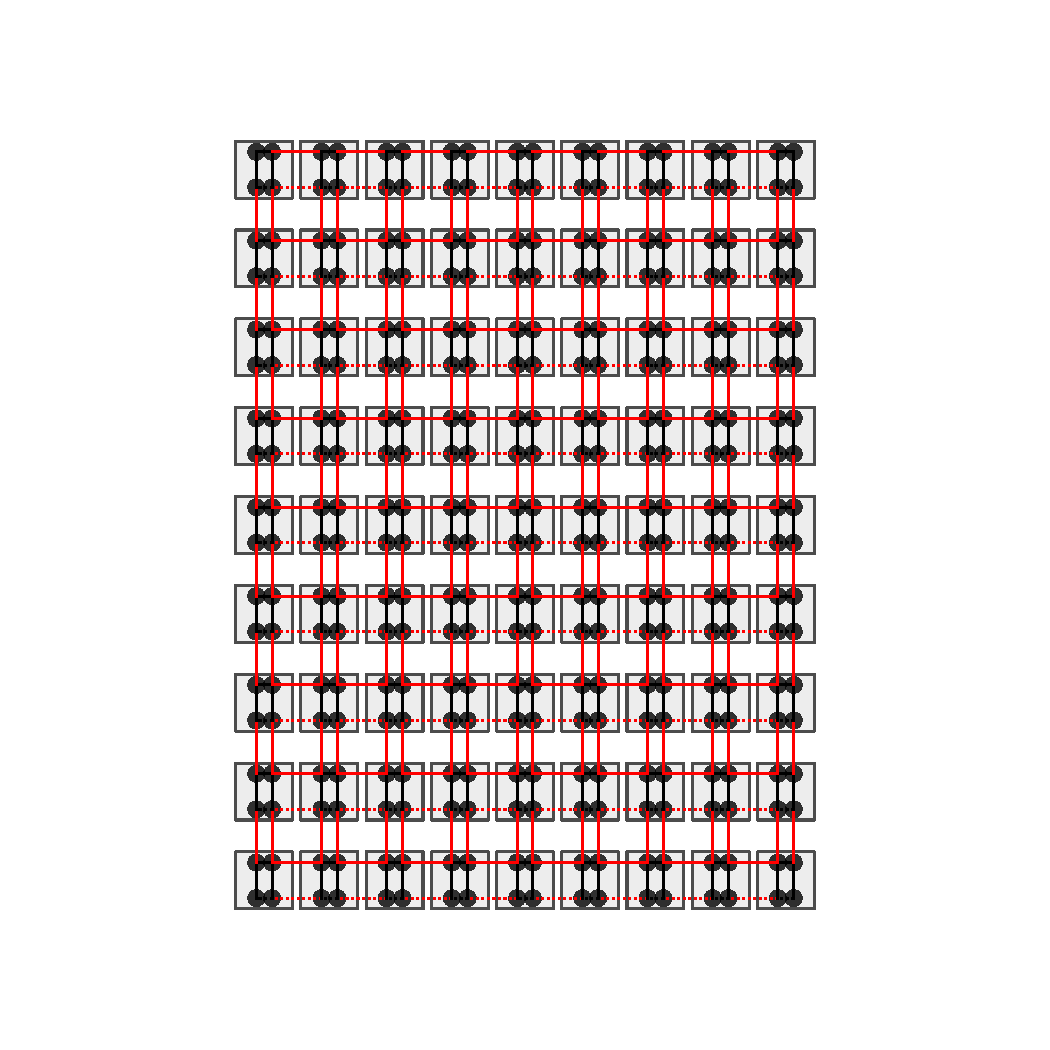
\includegraphics[width=\textwidth]{Imagenes/Models/Model_pump/square_pump_model_x_0.pdf}
         \end{subfigure}\hspace*{-0.5em}
         \begin{subfigure}[b!]{0.2 \textwidth}
             \caption*{}
             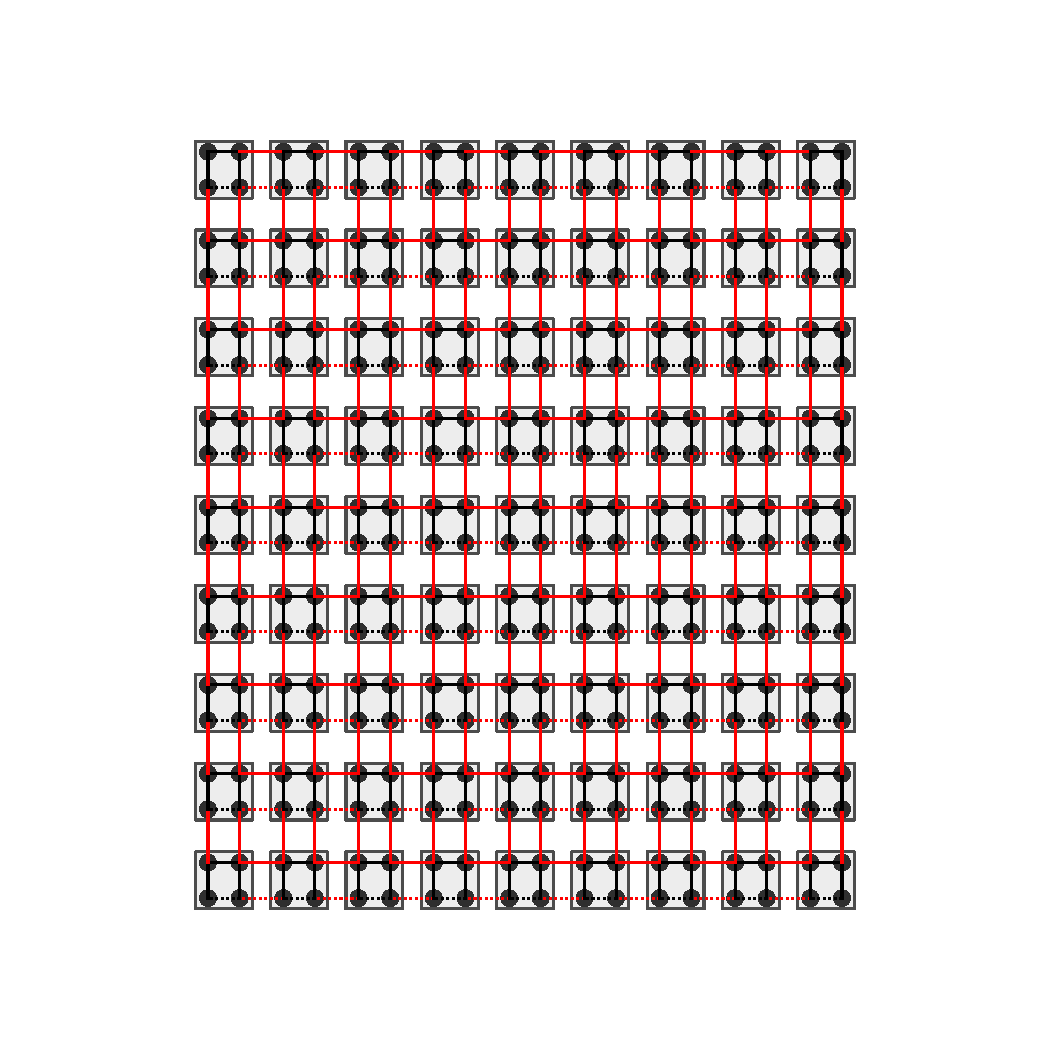
\includegraphics[width=\textwidth]{Imagenes/Models/Model_pump/square_pump_model_x_5.pdf}
         \end{subfigure}\hspace*{-0.5em}
         \begin{subfigure}[b!]{0.2 \textwidth}
             \caption*{}
             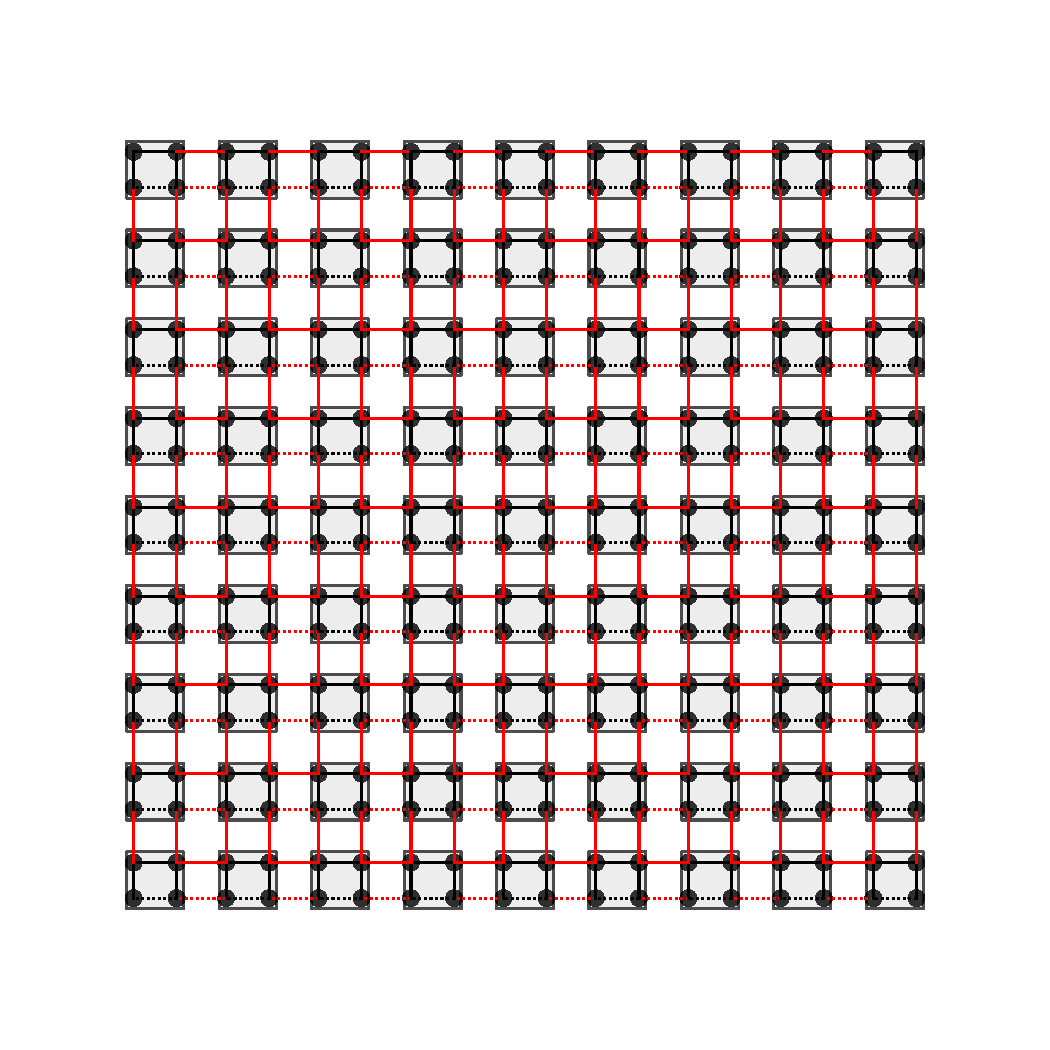
\includegraphics[width=\textwidth]{Imagenes/Models/Model_pump/square_pump_model_x_8.pdf}
         \end{subfigure}\hspace*{-0.5em}
         \begin{subfigure}[b!]{0.2 \textwidth}
             \caption*{}
             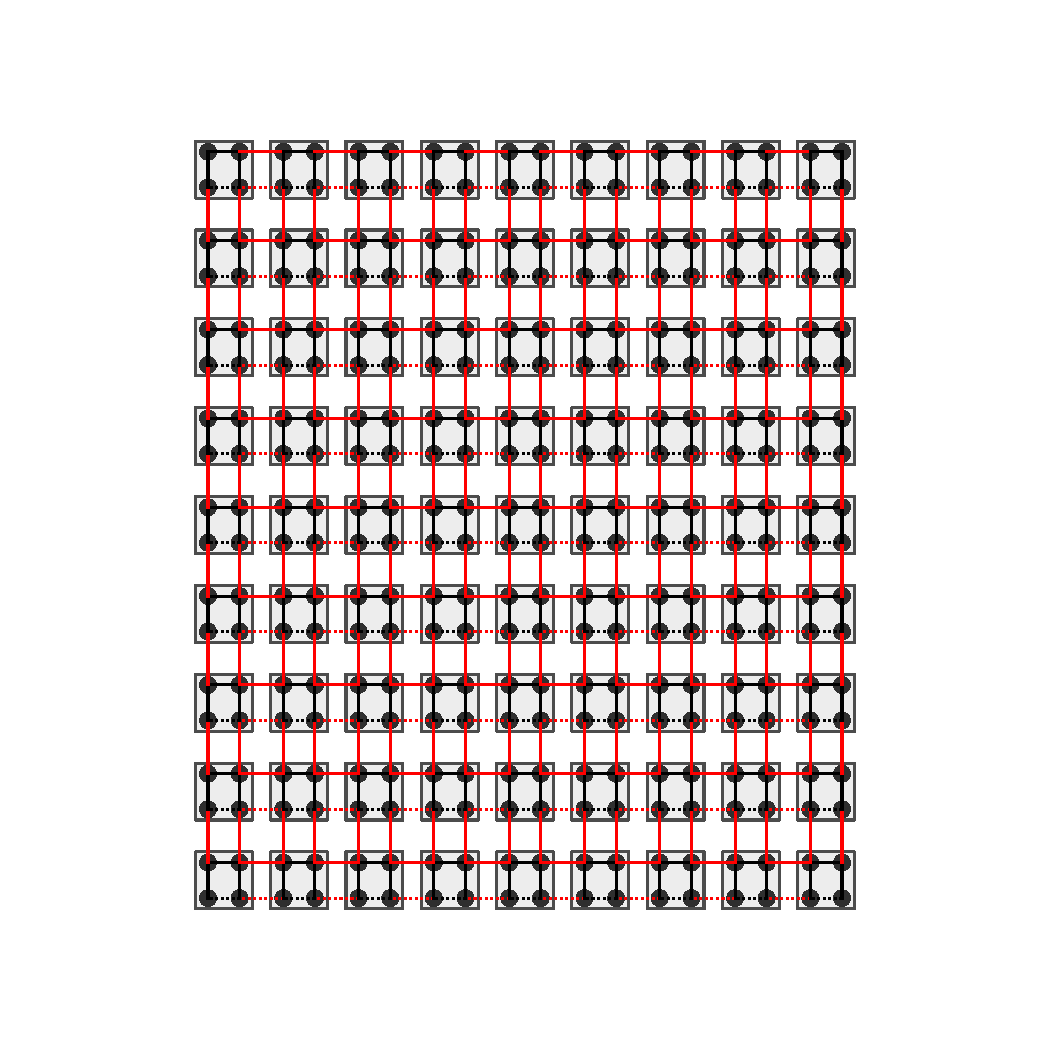
\includegraphics[width=\textwidth]{Imagenes/Models/Model_pump/square_pump_model_x_11.pdf}
         \end{subfigure}\hspace*{-0.5em}
         \begin{subfigure}[b!]{0.2 \textwidth}
             \caption*{}
             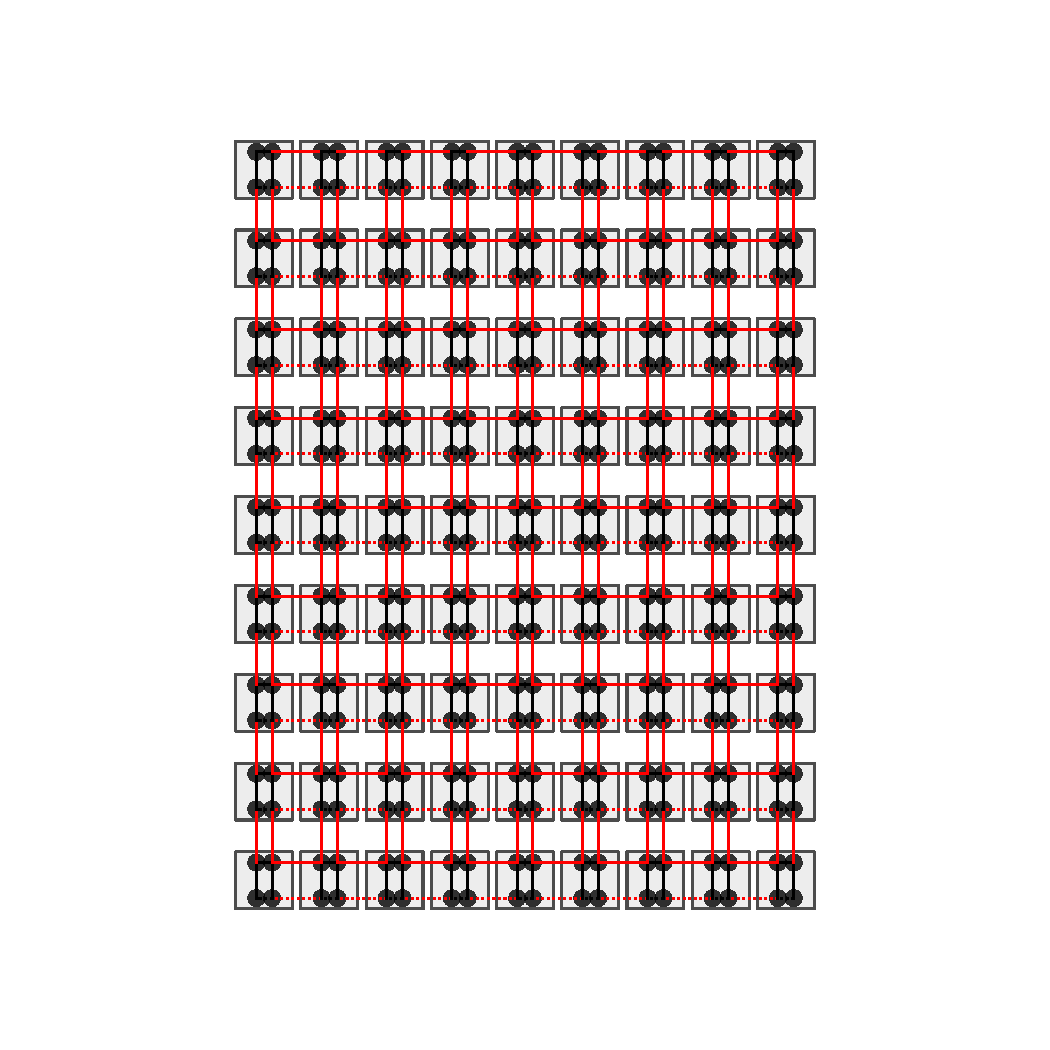
\includegraphics[width=\textwidth]{Imagenes/Models/Model_pump/square_pump_model_x_16.pdf}
         \end{subfigure}\hspace*{-0.5em}
     \end{minipage}\vspace*{-1em}
     
     
     \begin{minipage}[h!]{1.0\textwidth}
         \begin{subfigure}[b!]{0.2 \textwidth}
             \caption{}
             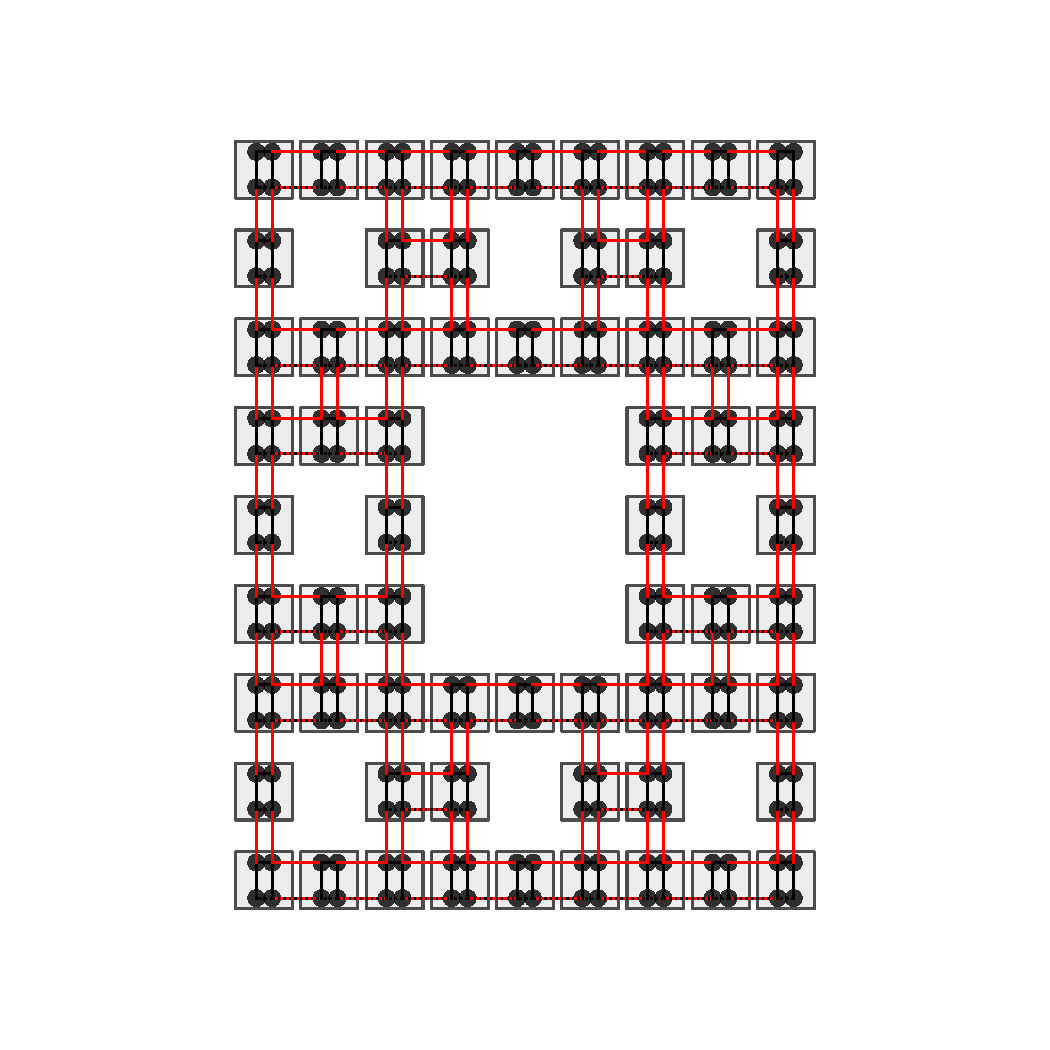
\includegraphics[width=\textwidth]{Imagenes/Models/Model_pump/fractal_pump_model_x_0.pdf}
         \end{subfigure}\hspace*{-0.5em}
         \begin{subfigure}[b!]{0.2 \textwidth}
             \caption*{}
             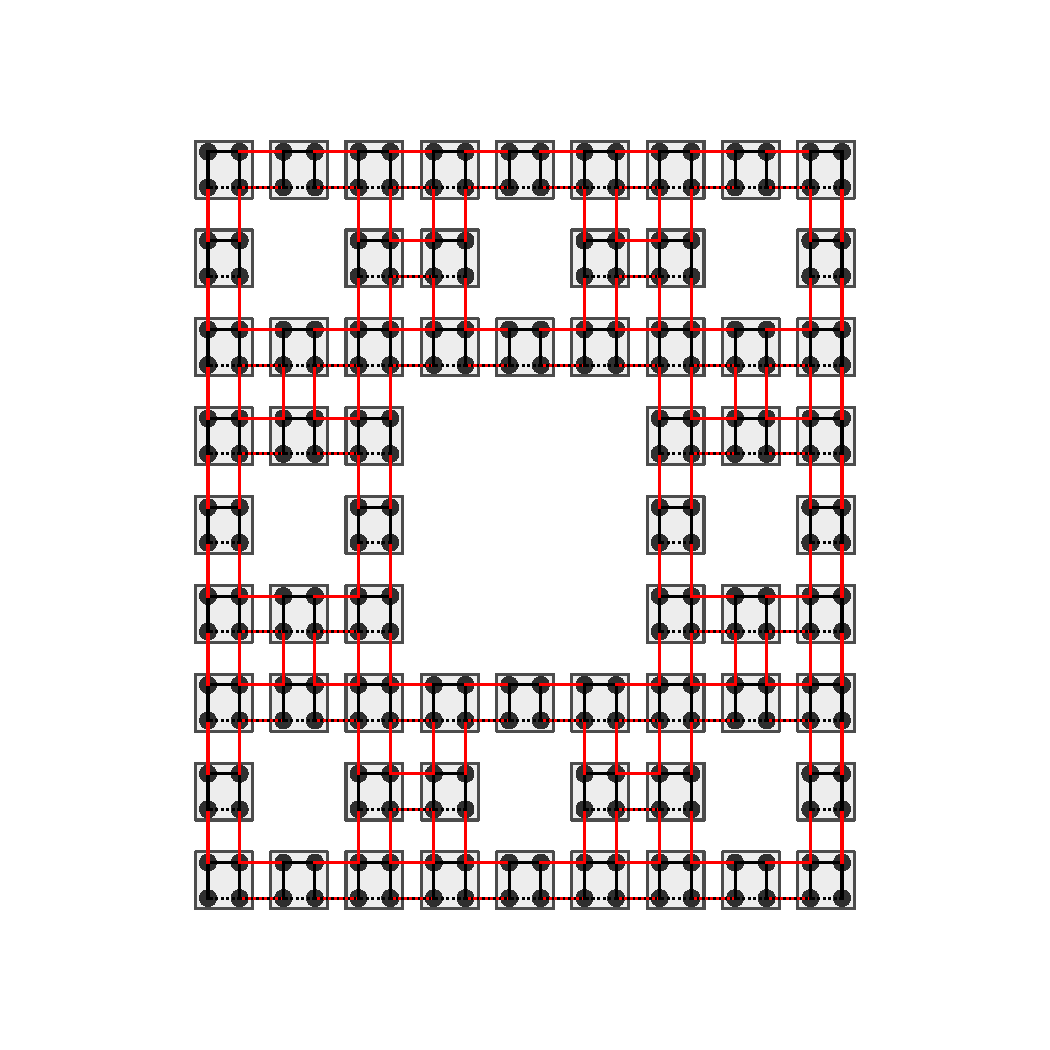
\includegraphics[width=\textwidth]{Imagenes/Models/Model_pump/fractal_pump_model_x_5.pdf}
         \end{subfigure}\hspace*{-0.5em}
         \begin{subfigure}[b!]{0.2 \textwidth}
             \caption*{}
             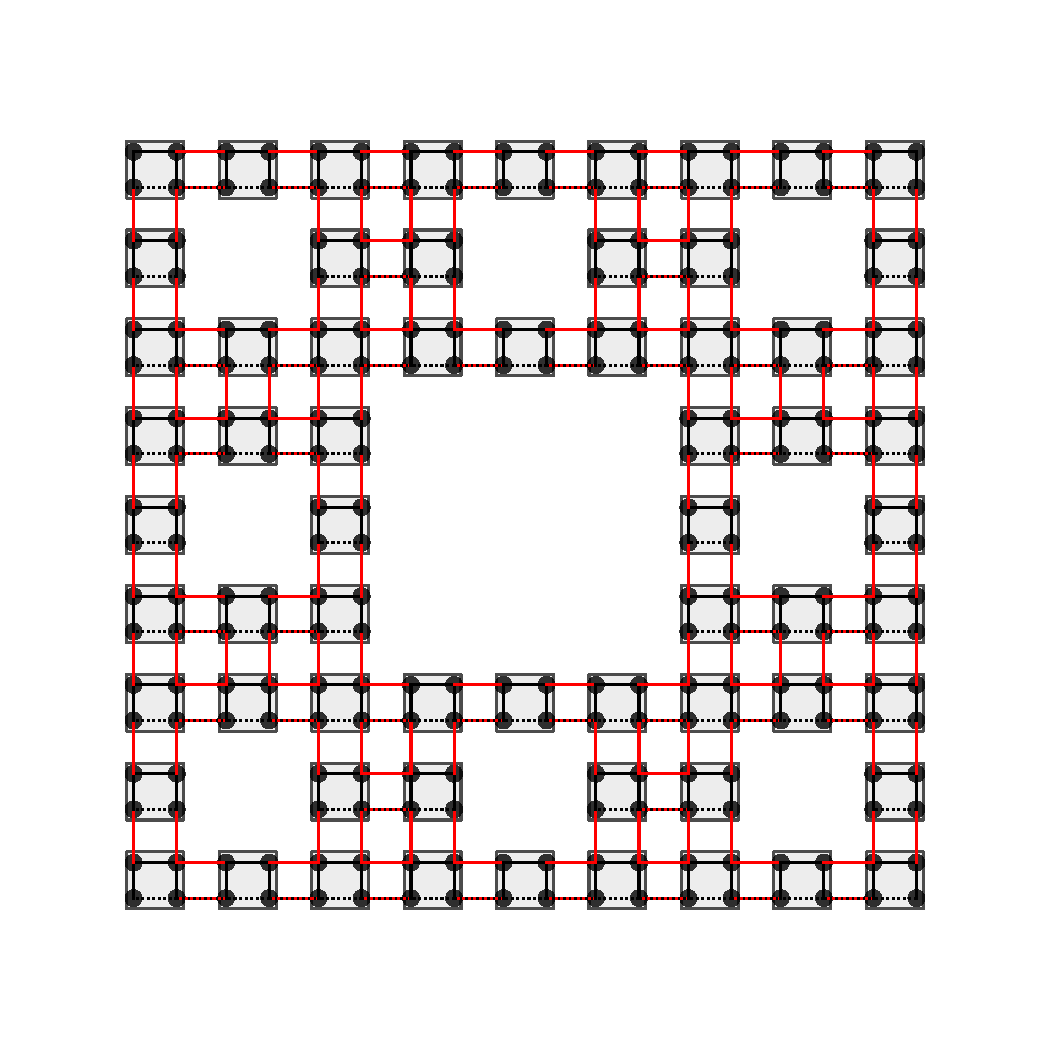
\includegraphics[width=\textwidth]{Imagenes/Models/Model_pump/fractal_pump_model_x_8.pdf}
         \end{subfigure}\hspace*{-0.5em}
         \begin{subfigure}[b!]{0.2 \textwidth}
             \caption*{}
             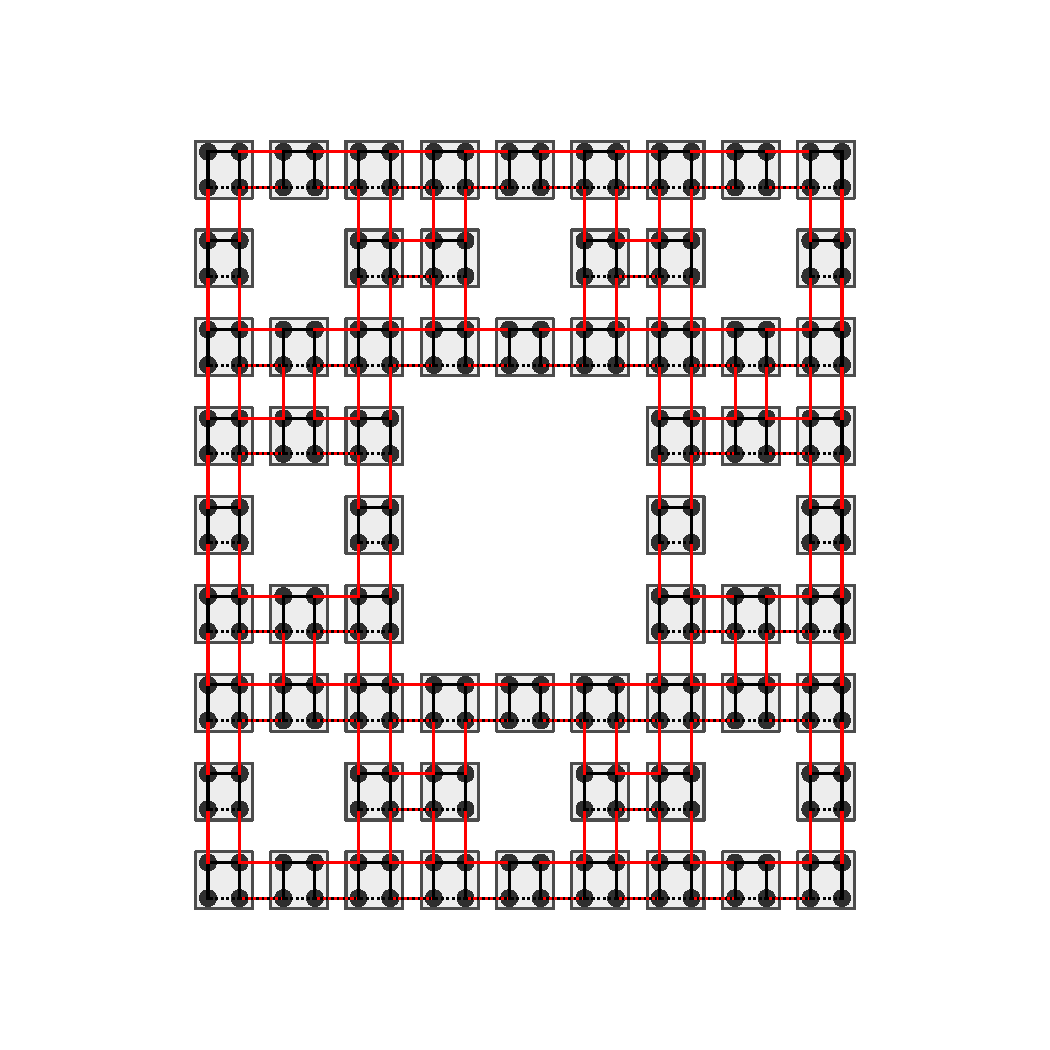
\includegraphics[width=\textwidth]{Imagenes/Models/Model_pump/fractal_pump_model_x_11.pdf}
         \end{subfigure}\hspace*{-0.5em}
         \begin{subfigure}[b!]{0.2 \textwidth}
             \caption*{}
             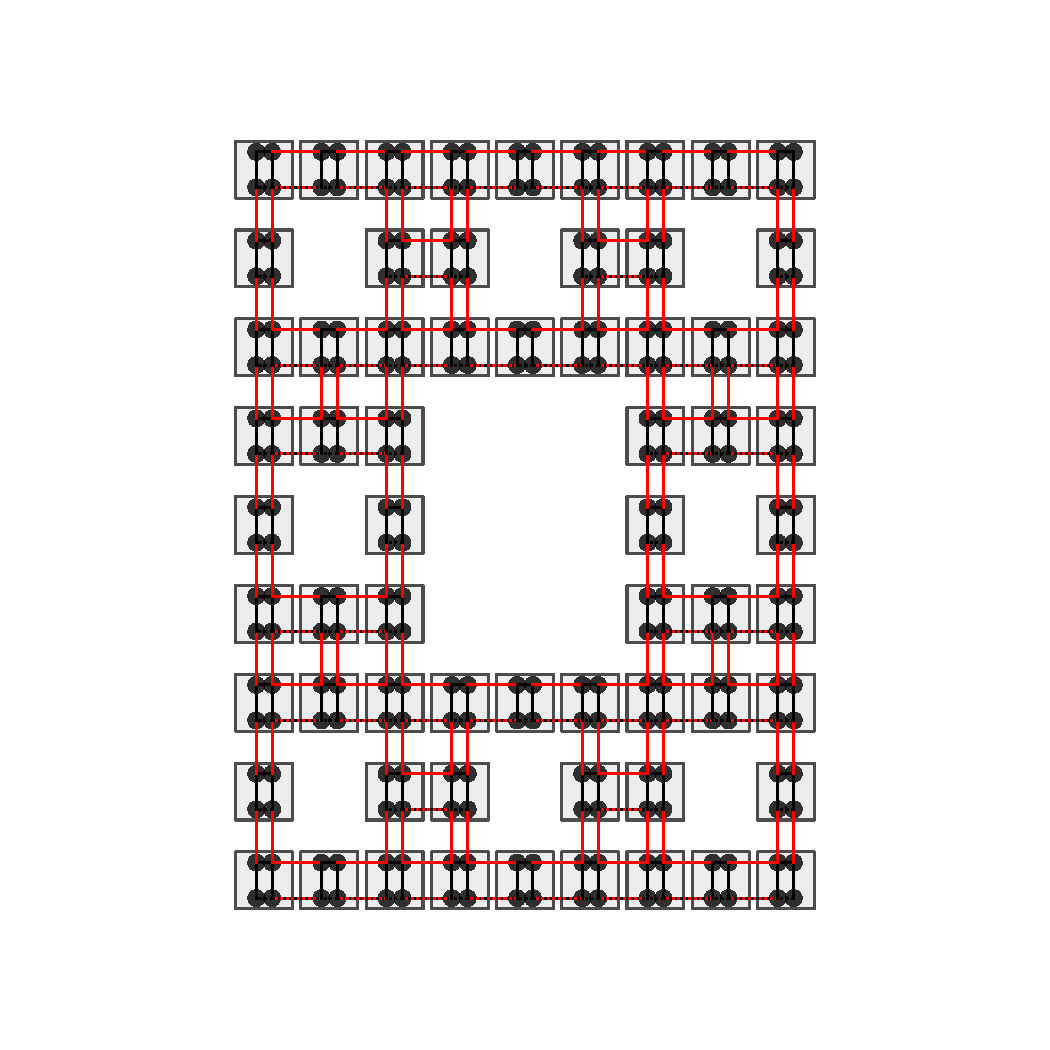
\includegraphics[width=\textwidth]{Imagenes/Models/Model_pump/fractal_pump_model_x_16.pdf}
         \end{subfigure}\hspace*{-0.5em}
     \end{minipage}\vspace*{-1em}
     
     \begin{minipage}[h!]{1.0\textwidth}
         \begin{subfigure}[b!]{0.2 \textwidth}
             \caption{}
             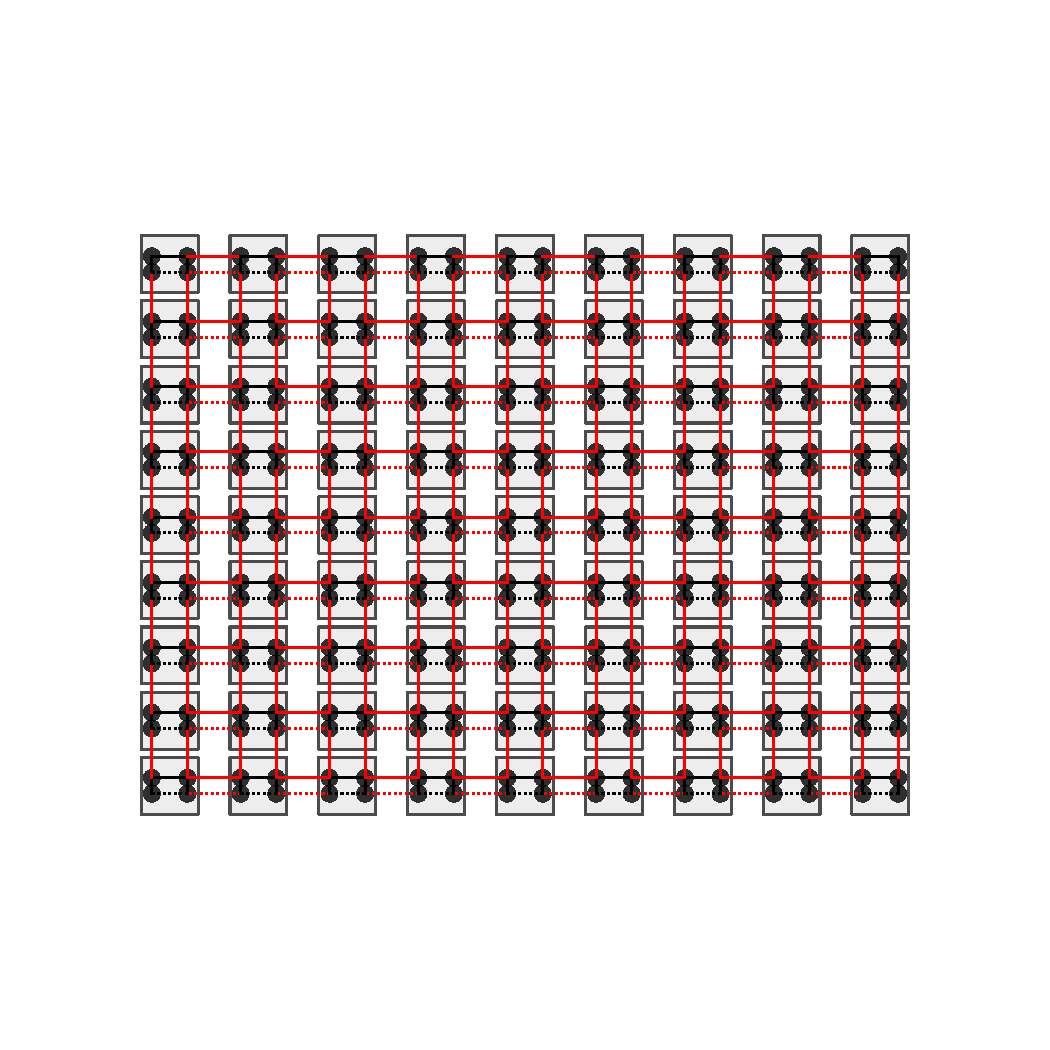
\includegraphics[width=\textwidth]{Imagenes/Models/Model_pump/square_pump_model_y_0.pdf}
         \end{subfigure}\hspace*{-0.5em}
         \begin{subfigure}[b!]{0.2 \textwidth}
             \caption*{}
             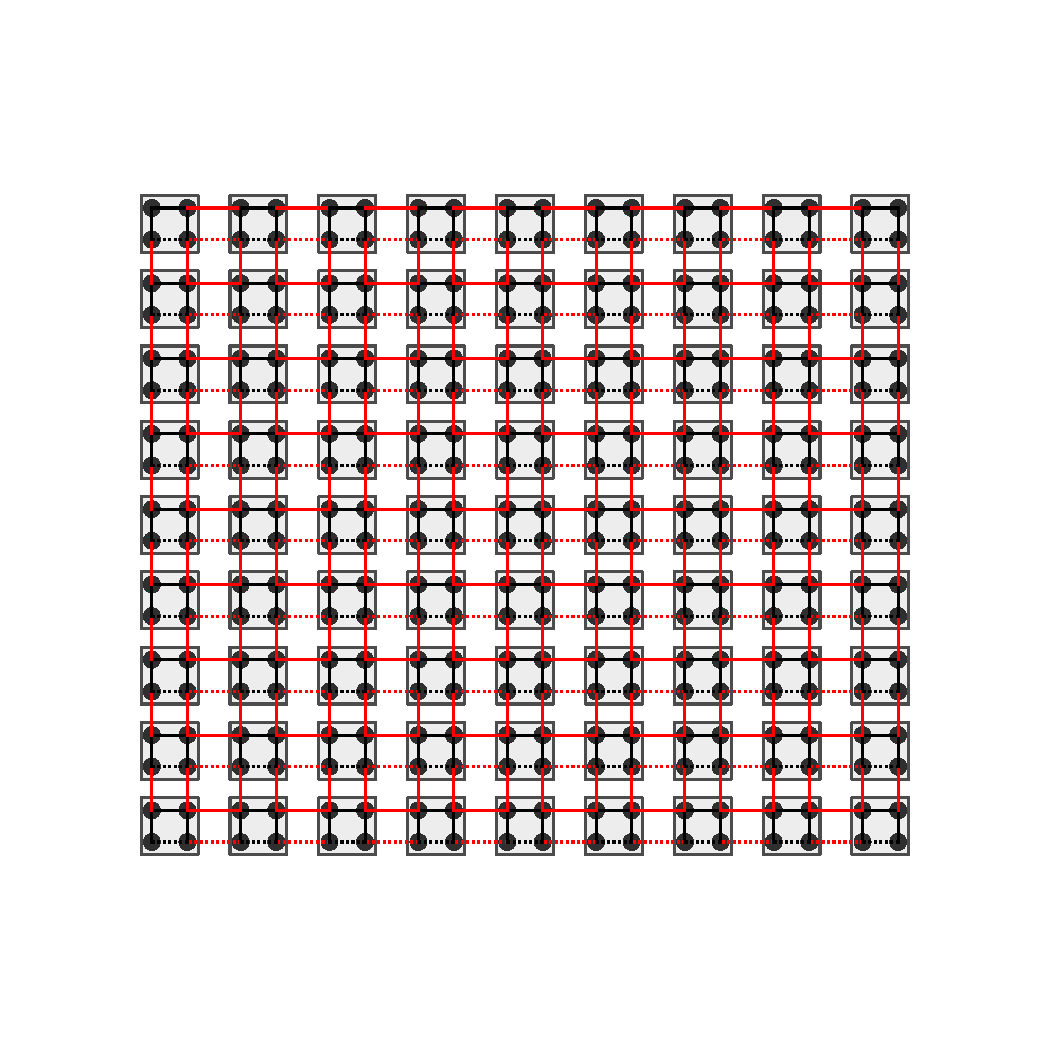
\includegraphics[width=\textwidth]{Imagenes/Models/Model_pump/square_pump_model_y_5.pdf}
         \end{subfigure}\hspace*{-0.5em}
         \begin{subfigure}[b!]{0.2 \textwidth}
             \caption*{}
             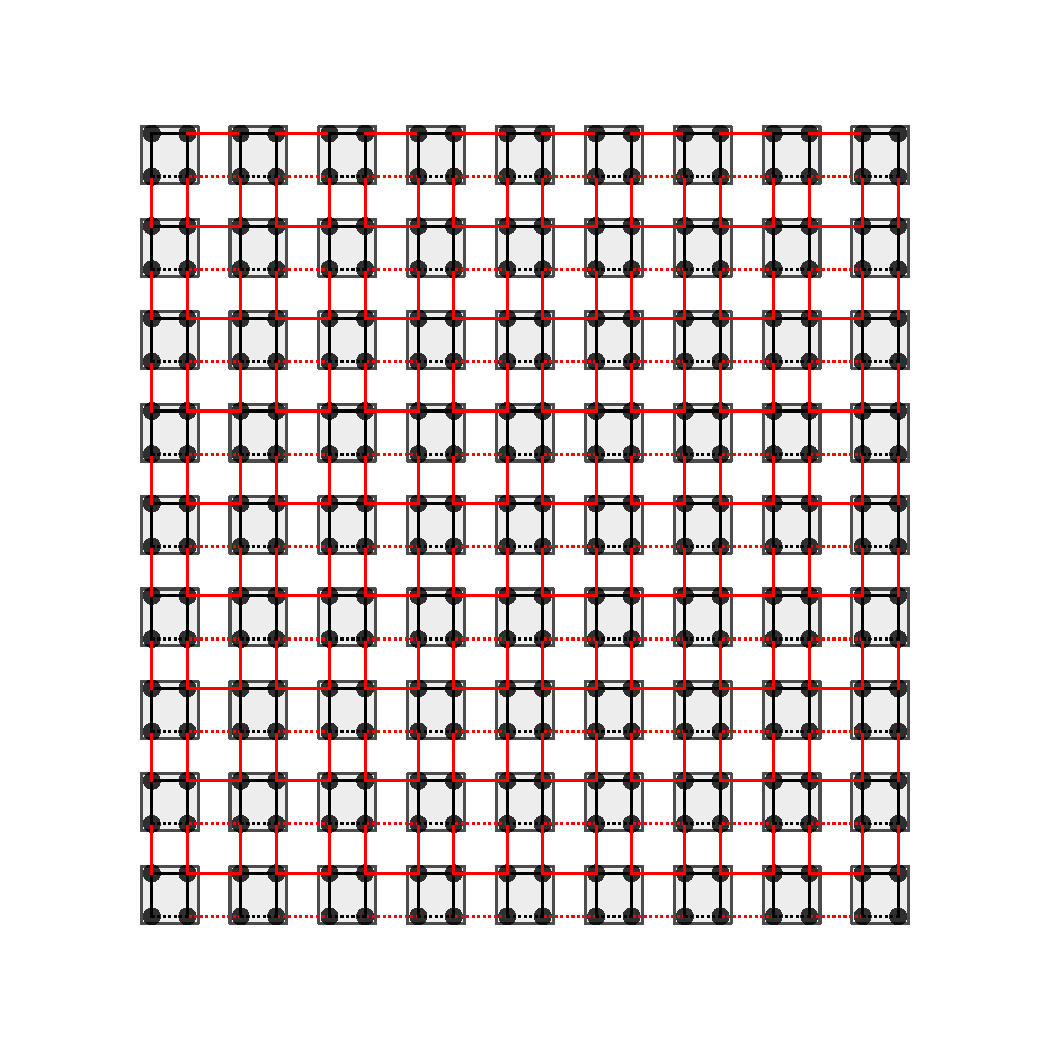
\includegraphics[width=\textwidth]{Imagenes/Models/Model_pump/square_pump_model_y_8.pdf}
         \end{subfigure}\hspace*{-0.5em}
         \begin{subfigure}[b!]{0.2 \textwidth}
             \caption*{}
             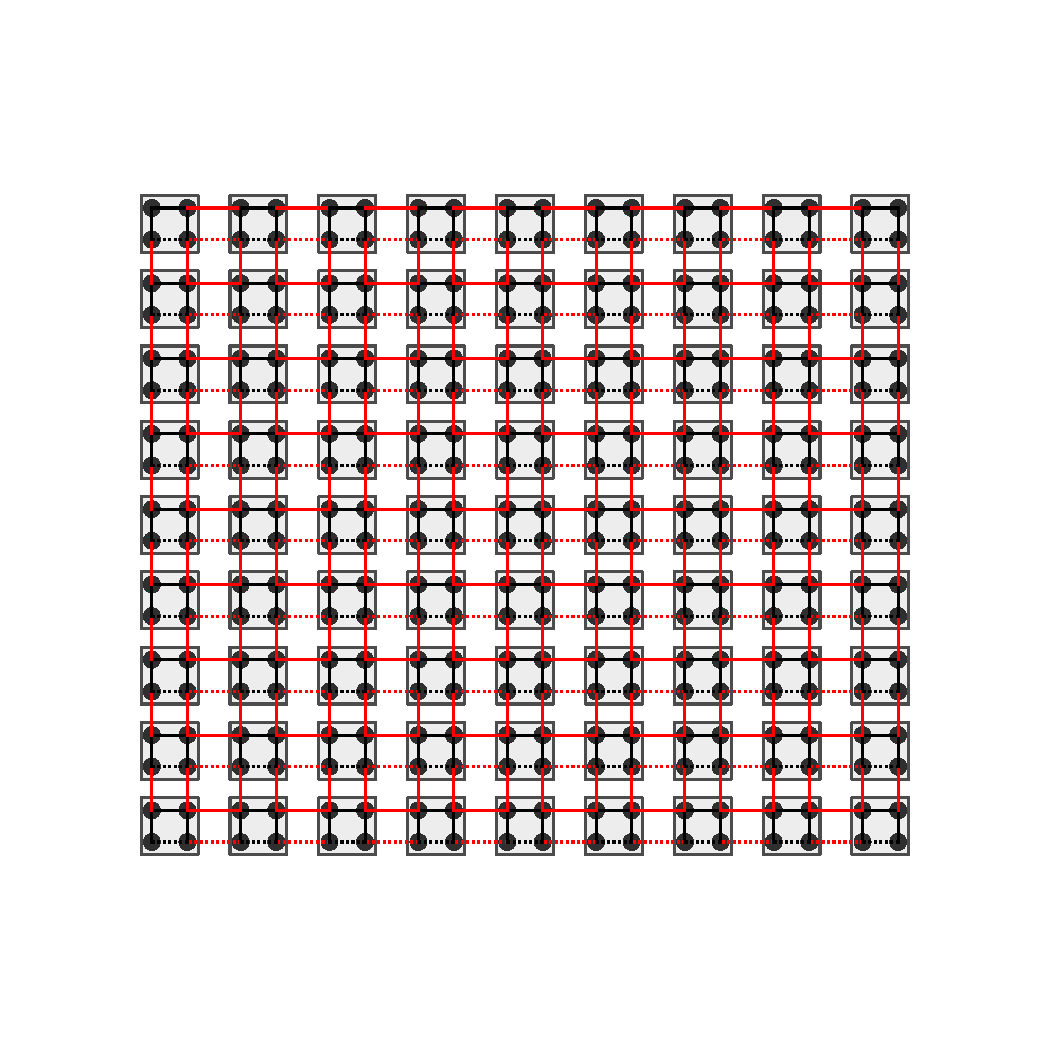
\includegraphics[width=\textwidth]{Imagenes/Models/Model_pump/square_pump_model_y_11.pdf}
         \end{subfigure}\hspace*{-0.5em}
         \begin{subfigure}[b!]{0.2 \textwidth}
             \caption*{}
             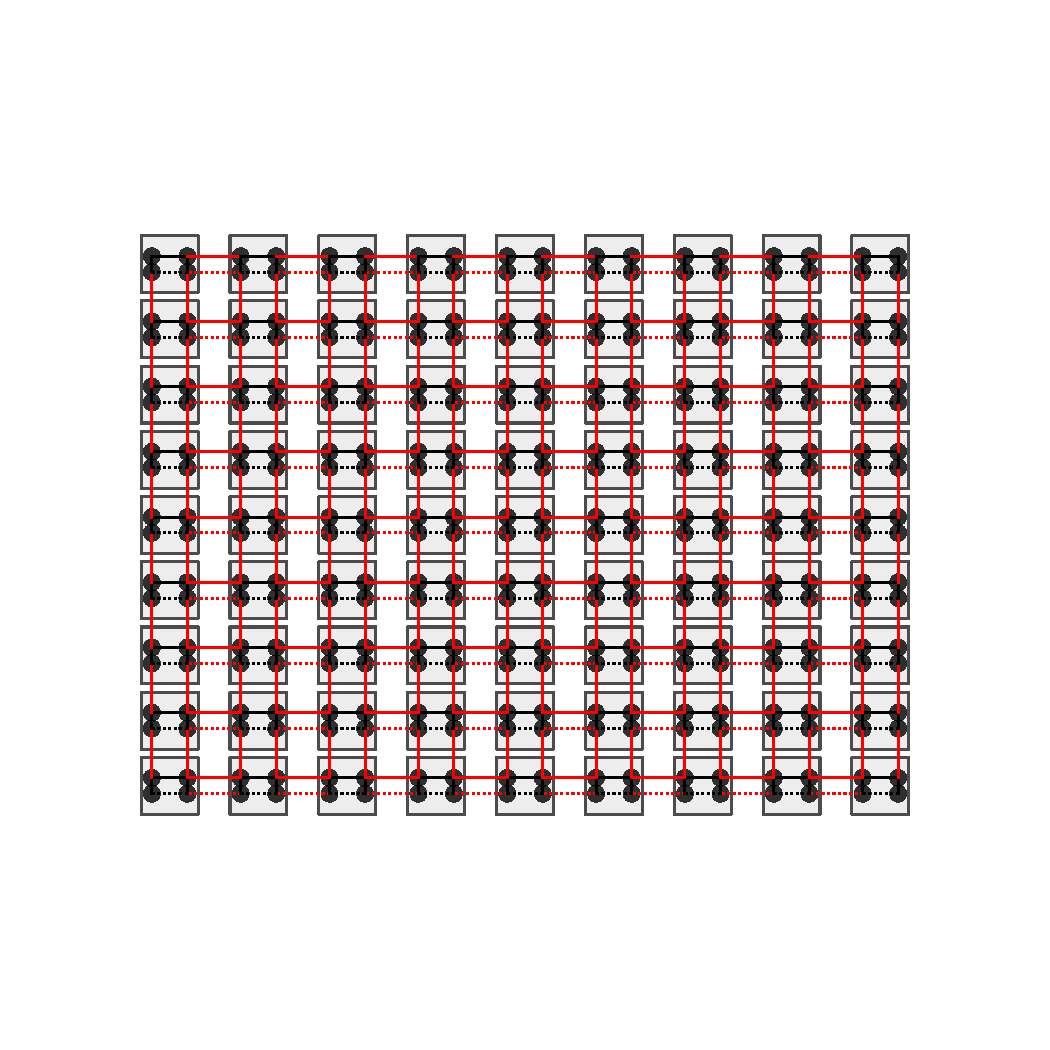
\includegraphics[width=\textwidth]{Imagenes/Models/Model_pump/square_pump_model_y_16.pdf}
         \end{subfigure}\hspace*{-0.5em}
     \end{minipage}\vspace*{-1em}
     
     
     \begin{minipage}[h!]{1.0\textwidth}
         \begin{subfigure}[b!]{0.2 \textwidth}
             \caption{}
             \includegraphics[width=\textwidth]{Imagenes/Models/Model_pump/fractal_pump_model_y_0.pdf}
         \end{subfigure}\hspace*{-0.5em}
         \begin{subfigure}[b!]{0.2 \textwidth}
             \caption*{}
             \includegraphics[width=\textwidth]{Imagenes/Models/Model_pump/fractal_pump_model_y_5.pdf}
         \end{subfigure}\hspace*{-0.5em}
         \begin{subfigure}[b!]{0.2 \textwidth}
             \caption*{}
             \includegraphics[width=\textwidth]{Imagenes/Models/Model_pump/fractal_pump_model_y_8.pdf}
         \end{subfigure}\hspace*{-0.5em}
         \begin{subfigure}[b!]{0.2 \textwidth}
             \caption*{}
             \includegraphics[width=\textwidth]{Imagenes/Models/Model_pump/fractal_pump_model_y_11.pdf}
         \end{subfigure}\hspace*{-0.5em}
         \begin{subfigure}[b!]{0.2 \textwidth}
             \caption*{}
             \includegraphics[width=\textwidth]{Imagenes/Models/Model_pump/fractal_pump_model_y_16.pdf}
         \end{subfigure}\hspace*{-0.5em}
     \end{minipage}\vspace*{-0.2em}     
    \caption{Variaciones de la geometría de las redes cristalinas cuadrada y fractal cuando varian los parametros de salto en las direcciones: \textbf{(a) - (b)} $\textbf{X}$ y $\textbf{Y}$, \textbf{(c) - (d)} $\textbf{X}$, \textbf{(e) - (f)} $\textbf{Y}$. }
    \label{fig:Model_pump}
\end{figure}

Como se menciono en la introducción existen trabajos recientes que muestran que las propiedades de transporte en aislantes topológicos de pueden presentar con estados protegidos por invariantes como el numero de Chern. En el articulo (High order topological pump), Benalcazar at al. muestran estas propiedades en un arreglo experimental con guías de ondas. Inspirados en esta idea decidimos introducir parámetros cíclicos similares a los de las guía de onda propuestos en este articulo en nuestro modelo del Hoti cuadrado y fractal.

In the conventional Thouless pump [26, 33], an insulator with discrete translation symmetry adiabatically
evolves in a periodic fashion leading to a quantization
of the electron transport per cycle. The transport can be
tracked by following the dipole moment in a crystal as the
cycle progresses [34]. The change of the dipole moment
over a cycle is a topologically-protected integer equal to
the Chern number of the energy bands calculated in the
2D manifold spanned by the crystal momentum and the
adiabatic parameter over that cycle [28].

%
% Resultados
%
\chapter{Resultados}

\begin{center}
\begin{minipage}{0.9\textwidth}
{\small
{\bf Resumen:} Resumen de resultados.
}
\end{minipage}
\end{center}

\section{Bulk HOTI cuadrado}



\subsection{Hoti Cuadrado}
%{\it Primero mencionar qué se grafica en la figura antes interpretarla.} Como se puede observar en la figura \ref{fig:Dos_cuadrado} la solución del modelo de SSH para el arreglo cuadrado (figura) arroja una clara transición de fase electrónica conforme los parámetros de salto $\gamma/\lambda$ varían. Para valores de $\gamma/\lambda < 1$ podemos observar 4 estados en el centro lo cual indicaría una fase topológica estos estados carecen de brecha energética, estos estados se deben a finitud geométrica del arreglo. Para valores de $\gamma/\lambda = 0$ tendríamos el caso limite en el que tenemos un fase semimetálica y para valores de $\gamma/\lambda > 1$ tendríamos una fase aislante o fase trivial.
\begin{figure}[h!]
     \centering
    \captionsetup[sub]{font=small}
     \begin{subfigure}[b!]{0.3 \textwidth}
         \caption{}
         \includegraphics[width=\textwidth]{Imagenes/Resultados_Hoti_Cuadrado/bars_square1.pdf}
     \end{subfigure}\hspace*{1em}
     \begin{subfigure}[b!]{0.3 \textwidth}
         \caption{}
         \includegraphics[width=\textwidth]{Imagenes/Resultados_Hoti_Cuadrado/bars_square2.pdf}
     \end{subfigure}\hspace*{1em}
     \begin{subfigure}[b!]{0.3 \textwidth}
         \caption{}
         \includegraphics[width=\textwidth]{Imagenes/Resultados_Hoti_Cuadrado/bars_square3.pdf}
     \end{subfigure}\hspace*{1em}\vspace*{-0.5em}
        \caption{Numero de estados por energía en un red con geometría cuadrada para diferentes valores de los parámetros de salto, \textbf{a)} $\gamma /\lambda = 1/2$, \textbf{b)} $\gamma /\lambda = 1$, \textbf{c)} $\gamma /\lambda = 2$.}
        \label{fig:Dos_Cuadrado}
\end{figure}
En la figura \ref{fig:Dos_Cuadrado} podemos ver el numero de estados por energía en el modelo de BBT para una red cuadrada \ref{Modelo_SSH_square_and_Fractal} para diferentes valores de $\gamma/\lambda$. Para los valores de $\gamma/\lambda>1$ \ref{fig:Dos_Cuadrado} \texbf{c)} podemos ver un claro gap energético, lo cual indicaría que nuestra red cristalina se encuentra en un estado trivial, es decir, es un aislante común. Para los valores de $\gamma/\lambda<1$ \ref{fig:Dos_Cuadrado} \texbf{a)} aparecen 4 estados degenerados carentes de gap en la energía de Fermi, estos aparecen como consecuencia de la finitud de la red cristalina por lo que les llamaremos estados de borde, esta fase del la red es conocida como fase topológica. En la figura \ref{fig:Dos_Cuadrado} para  \texbf{a)} $\gamma/\lambda = 1$ vemos que el gap energético de la red cristalina se cierra, lo cual indica la posible transición de fase entre el estado topológico y trivial con la variación de los parámetros de salto $\gamma/\lambda$ de la red cristalina.


\begin{figure}[h!]
     \centering
    \captionsetup[sub]{font=small}
     \begin{subfigure}[b!]{0.44 \textwidth}
         \caption{}
         \includegraphics[width=\textwidth]{Imagenes/Resultados_Hoti_Cuadrado/bands_square_shh.pdf}
         \label{}
     \end{subfigure}\hspace*{1em}
     \begin{subfigure}[b!]{0.56 \textwidth}
         \caption{}
         \includegraphics[width=\textwidth]{Imagenes/Resultados_Hoti_Cuadrado/proyection_square.pdf}
         \label{}
     \end{subfigure}\hspace*{1em} \vspace*{-1.5em}
        \caption{\textbf{a)}Espectro de energía del sistema con geometría cuadrada y condiciones abiertas a la frontera, como función de $\gamma/\lambda$. Las energías centrales coloreadas en rojo corresponde a los 4 estados localizados en las esquinas. \textbf{b)} Densidad de probabilidad en un fase no trivial donde $\gamma = 1,\, \, \lambda = 4.5$, en un red cuadrada de $18\times18$ sitios.}
    \label{fig:Pram_Proy_cuadrado}
\end{figure}



Para ver mas a detalle como sucede esta transición de fase podemos hacer un seguimiento del espectro de energías conforme se varían los parámetros de salto y enfocarnos en las energías centrales correspondientes a los estados de borde Figura \ref{fig:Pram_Proy_cuadrado} \texbf{(a)}. Las energías centrales están coloreadas con azul en la zona trivial y rojo en la zona topológica, en la zona $|\gamma/\lambda|>1$ el comportamiento de estas energías es similar a las energías de los estados del bulto de la red cristalna, sin embargo, en la zona $|\gamma/\lambda|>1$ las energías centrales se degeneran en la energía de Fermi, al proyectar las densidades de probabilidad de los estados correspondientes a estas 4 energías obtenemos la figura \ref{fig:Pram_Proy_cuadrado} \texbf{(b)} donde las densidades se encuentran claramente localizadas en las equinas de la red con probabilidad de aproximadamente $1/4$, lo cual definiria a nuestra red cirstalina como un aislante topológico de orden superior (HOTI \footnote{Siglas en ingles de High Order Topological Insulator}), donde el valor máximo de $\rho_{corner} = 1/4$ se alcanza en el caso limite $|\gamma/\lambda| = 0$ donde las celdas estarían totalmente cuatrimerizadas.

También estos estados son robustos ante perturbaciones como se puede observar en la figura \ref{fig:para_proy_Delta_fractal} \texbf{(a)-(e)} donde las perturbaciones se ejercieron sobre los parámetros de salto $\gamma' = \gamma( 1 \pm \epsilon) ,\, \, \lambda' = \lambda( 1 \pm \epsilon)$, \comA{Simetrias}, como se puede ver estas variaciones solo cambian las energías correspondientes a los estados del bulto y no a los estados de borde que permanecen robustos, así como en la proyección de la densidad de probabilidad en el espacio real se mantienen inalterados los estados localizados en las esquinas.


\vspace{1cm}
    \begin{figure}[thb!]
        \centering
        \begin{minipage}{0.8\textwidth}
           \captionsetup[sub]{font=small}
            \begin{minipage}[h!]{0.8\textwidth}
                \begin{subfigure}[b!]{0.44 \textwidth}
                    \caption{$\epsilon = 1\%$}
                    \includegraphics[width=\textwidth]{Imagenes/Resultados_Hoti_Cuadrado/bands_square_shh_0.01.pdf}
                \end{subfigure}\hspace*{-0.5em}
                \begin{subfigure}[b!]{0.56 \textwidth}
                    \caption*{}
                    \includegraphics[width=\textwidth]{Imagenes/Resultados_Hoti_Cuadrado/proyection_square_0.01.pdf}
                \end{subfigure}\hspace*{-0.5em}
            \end{minipage}\vspace*{-1.5em}
            
            \begin{minipage}[h!]{0.8\textwidth}
                \begin{subfigure}[b!]{0.44 \textwidth}
                    \caption{$\epsilon = 5\%$}
                    \includegraphics[width=\textwidth]{Imagenes/Resultados_Hoti_Cuadrado/bands_square_shh_0.05.pdf}
                \end{subfigure}\hspace*{-0.5em}
                \begin{subfigure}[b!]{0.56 \textwidth}
                    \caption*{}
                    \includegraphics[width=\textwidth]{Imagenes/Resultados_Hoti_Cuadrado/proyection_square_0.05.pdf}
                \end{subfigure}\hspace*{-0.5em}
            \end{minipage}\vspace*{-1.5em}
            
            \begin{minipage}[h!]{0.8\textwidth}
                \begin{subfigure}[b!]{0.44 \textwidth}
                    \caption{$\epsilon = 10\%$}
                    \includegraphics[width=\textwidth]{Imagenes/Resultados_Hoti_Cuadrado/bands_square_shh_0.1.pdf}
                \end{subfigure}\hspace*{-0.5em}
                \begin{subfigure}[b!]{0.56 \textwidth}
                    \caption*{}
                    \includegraphics[width=\textwidth]{Imagenes/Resultados_Hoti_Cuadrado/proyection_square_0.1.pdf}
                \end{subfigure}\hspace*{-0.5em}
            \end{minipage}\vspace*{-1.5em}
            
            \begin{minipage}[h!]{0.8\textwidth}
                \begin{subfigure}[b!]{0.44 \textwidth}
                    \caption{$\epsilon = 30\%$}
                    \includegraphics[width=\textwidth]{Imagenes/Resultados_Hoti_Cuadrado/bands_square_shh_0.3.pdf}
                \end{subfigure}\hspace*{-0.5em}
                \begin{subfigure}[b!]{0.56 \textwidth}
                    \caption*{}
                    \includegraphics[width=\textwidth]{Imagenes/Resultados_Hoti_Cuadrado/proyection_square_0.3.pdf}
                \end{subfigure}\hspace*{-0.5em}
            \end{minipage}\vspace*{-1.5em}
            
            \begin{minipage}[h!]{0.8\textwidth}
                \begin{subfigure}[b!]{0.44 \textwidth}
                    \caption{$\epsilon = 50\%$}
                    \includegraphics[width=\textwidth]{Imagenes/Resultados_Hoti_Cuadrado/bands_square_shh_0.5.pdf}
                \end{subfigure}\hspace*{-0.5em}
                \begin{subfigure}[b!]{0.56 \textwidth}
                    \caption*{}
                    \includegraphics[width=\textwidth]{Imagenes/Resultados_Hoti_Cuadrado/proyection_square_0.5.pdf}
                \end{subfigure}\hspace*{-0.5em}
            \end{minipage}\vspace*{-0.5em}
        \end{minipage} 
           \caption{\textbf{(a)-(e)}En la columna derecha se muestra el espectro de energías en una red cuadrada como función de $\gamma/\lambda $ con un desorden aleatorio en los parámetros de salto, de tamaño $\delta$. Las lineas rojas corresponden a los cuatro estados degenerados que representan los estados localizados en las esquinas. En la columna izquierda se muestra la densidad de probabilidad de la fase no trivial donde $\gamma' = \gamma( 1 \pm \epsilon) ,\, \, \lambda' = \lambda( 1 \pm \epsilon)$.  }
           \label{fig:Pram_Proy_Delta_cuadrado}
         
       \end{figure} 

    





 %\renewcommand{\thesubfigure}{\roman{subfigure}}
\begin{figure}[h!]
     \centering
    \captionsetup[sub]{font=small}
     \begin{minipage}[h!]{1\textwidth}
         \begin{subfigure}[b!]{0.2 \textwidth}
             \caption{$\theta = - \pi$}
             \includegraphics[width=\textwidth]{Imagenes/Models/Model_pump/square_pump_model_xy_0.pdf}
         \end{subfigure}\hspace*{-0.5em}
         \begin{subfigure}[b!]{0.2 \textwidth}
             \caption*{$\theta = -\frac{\pi}{2}$}
             \includegraphics[width=\textwidth]{Imagenes/Models/Model_pump/square_pump_model_xy_5.pdf}
         \end{subfigure}\hspace*{-0.5em}
         \begin{subfigure}[b!]{0.2 \textwidth}
             \caption*{$\theta = 0$}
             \includegraphics[width=\textwidth]{Imagenes/Models/Model_pump/square_pump_model_xy_8.pdf}
         \end{subfigure}\hspace*{-0.5em}
         \begin{subfigure}[b!]{0.2 \textwidth}
             \caption*{$\theta = \frac{\pi}{2}$}
             \includegraphics[width=\textwidth]{Imagenes/Models/Model_pump/square_pump_model_xy_11.pdf}
         \end{subfigure}\hspace*{-0.5em}
         \begin{subfigure}[b!]{0.2 \textwidth}
             \caption*{$\theta = \pi$}
             \includegraphics[width=\textwidth]{Imagenes/Models/Model_pump/square_pump_model_xy_16.pdf}
         \end{subfigure}\hspace*{-0.5em}
     \end{minipage}\vspace*{-1em}
     
     
     \begin{minipage}[h!]{1\textwidth}
         \begin{subfigure}[b!]{0.2 \textwidth}
             \caption{}
             \includegraphics[width=\textwidth]{Imagenes/Models/Model_pump/fractal_pump_model_xy_0.pdf}
         \end{subfigure}\hspace*{-0.5em}
         \begin{subfigure}[b!]{0.2 \textwidth}
             \caption*{}
             \includegraphics[width=\textwidth]{Imagenes/Models/Model_pump/fractal_pump_model_xy_5.pdf}
         \end{subfigure}\hspace*{-0.5em}
         \begin{subfigure}[b!]{0.2 \textwidth}
             \caption*{}
             \includegraphics[width=\textwidth]{Imagenes/Models/Model_pump/fractal_pump_model_xy_8.pdf}
         \end{subfigure}\hspace*{-0.5em}
         \begin{subfigure}[b!]{0.2 \textwidth}
             \caption*{}
             \includegraphics[width=\textwidth]{Imagenes/Models/Model_pump/fractal_pump_model_xy_11.pdf}
         \end{subfigure}\hspace*{-0.5em}
         \begin{subfigure}[b!]{0.2 \textwidth}
             \caption*{}
             \includegraphics[width=\textwidth]{Imagenes/Models/Model_pump/fractal_pump_model_xy_16.pdf}
         \end{subfigure}\hspace*{-0.5em}
     \end{minipage}\vspace*{-1em}
     
     
     \begin{minipage}[h!]{1.0\textwidth}
         \begin{subfigure}[b!]{0.2 \textwidth}
             \caption{}
             \includegraphics[width=\textwidth]{Imagenes/Models/Model_pump/square_pump_model_x_0.pdf}
         \end{subfigure}\hspace*{-0.5em}
         \begin{subfigure}[b!]{0.2 \textwidth}
             \caption*{}
             \includegraphics[width=\textwidth]{Imagenes/Models/Model_pump/square_pump_model_x_5.pdf}
         \end{subfigure}\hspace*{-0.5em}
         \begin{subfigure}[b!]{0.2 \textwidth}
             \caption*{}
             \includegraphics[width=\textwidth]{Imagenes/Models/Model_pump/square_pump_model_x_8.pdf}
         \end{subfigure}\hspace*{-0.5em}
         \begin{subfigure}[b!]{0.2 \textwidth}
             \caption*{}
             \includegraphics[width=\textwidth]{Imagenes/Models/Model_pump/square_pump_model_x_11.pdf}
         \end{subfigure}\hspace*{-0.5em}
         \begin{subfigure}[b!]{0.2 \textwidth}
             \caption*{}
             \includegraphics[width=\textwidth]{Imagenes/Models/Model_pump/square_pump_model_x_16.pdf}
         \end{subfigure}\hspace*{-0.5em}
     \end{minipage}\vspace*{-1em}
     
     
     \begin{minipage}[h!]{1.0\textwidth}
         \begin{subfigure}[b!]{0.2 \textwidth}
             \caption{}
             \includegraphics[width=\textwidth]{Imagenes/Models/Model_pump/fractal_pump_model_x_0.pdf}
         \end{subfigure}\hspace*{-0.5em}
         \begin{subfigure}[b!]{0.2 \textwidth}
             \caption*{}
             \includegraphics[width=\textwidth]{Imagenes/Models/Model_pump/fractal_pump_model_x_5.pdf}
         \end{subfigure}\hspace*{-0.5em}
         \begin{subfigure}[b!]{0.2 \textwidth}
             \caption*{}
             \includegraphics[width=\textwidth]{Imagenes/Models/Model_pump/fractal_pump_model_x_8.pdf}
         \end{subfigure}\hspace*{-0.5em}
         \begin{subfigure}[b!]{0.2 \textwidth}
             \caption*{}
             \includegraphics[width=\textwidth]{Imagenes/Models/Model_pump/fractal_pump_model_x_11.pdf}
         \end{subfigure}\hspace*{-0.5em}
         \begin{subfigure}[b!]{0.2 \textwidth}
             \caption*{}
             \includegraphics[width=\textwidth]{Imagenes/Models/Model_pump/fractal_pump_model_x_16.pdf}
         \end{subfigure}\hspace*{-0.5em}
     \end{minipage}\vspace*{-1em}
     
     \begin{minipage}[h!]{1.0\textwidth}
         \begin{subfigure}[b!]{0.2 \textwidth}
             \caption{}
             \includegraphics[width=\textwidth]{Imagenes/Models/Model_pump/square_pump_model_y_0.pdf}
         \end{subfigure}\hspace*{-0.5em}
         \begin{subfigure}[b!]{0.2 \textwidth}
             \caption*{}
             \includegraphics[width=\textwidth]{Imagenes/Models/Model_pump/square_pump_model_y_5.pdf}
         \end{subfigure}\hspace*{-0.5em}
         \begin{subfigure}[b!]{0.2 \textwidth}
             \caption*{}
             \includegraphics[width=\textwidth]{Imagenes/Models/Model_pump/square_pump_model_y_8.pdf}
         \end{subfigure}\hspace*{-0.5em}
         \begin{subfigure}[b!]{0.2 \textwidth}
             \caption*{}
             \includegraphics[width=\textwidth]{Imagenes/Models/Model_pump/square_pump_model_y_11.pdf}
         \end{subfigure}\hspace*{-0.5em}
         \begin{subfigure}[b!]{0.2 \textwidth}
             \caption*{}
             \includegraphics[width=\textwidth]{Imagenes/Models/Model_pump/square_pump_model_y_16.pdf}
         \end{subfigure}\hspace*{-0.5em}
     \end{minipage}\vspace*{-1em}
     
     
     \begin{minipage}[h!]{1.0\textwidth}
         \begin{subfigure}[b!]{0.2 \textwidth}
             \caption{}
             \includegraphics[width=\textwidth]{Imagenes/Models/Model_pump/fractal_pump_model_y_0.pdf}
         \end{subfigure}\hspace*{-0.5em}
         \begin{subfigure}[b!]{0.2 \textwidth}
             \caption*{}
             \includegraphics[width=\textwidth]{Imagenes/Models/Model_pump/fractal_pump_model_y_5.pdf}
         \end{subfigure}\hspace*{-0.5em}
         \begin{subfigure}[b!]{0.2 \textwidth}
             \caption*{}
             \includegraphics[width=\textwidth]{Imagenes/Models/Model_pump/fractal_pump_model_y_8.pdf}
         \end{subfigure}\hspace*{-0.5em}
         \begin{subfigure}[b!]{0.2 \textwidth}
             \caption*{}
             \includegraphics[width=\textwidth]{Imagenes/Models/Model_pump/fractal_pump_model_y_11.pdf}
         \end{subfigure}\hspace*{-0.5em}
         \begin{subfigure}[b!]{0.2 \textwidth}
             \caption*{}
             \includegraphics[width=\textwidth]{Imagenes/Models/Model_pump/fractal_pump_model_y_16.pdf}
         \end{subfigure}\hspace*{-0.5em}
     \end{minipage}\vspace*{-0.2em}     
    \caption{Variaciones de la geometría de las redes cristalinas cuadrada y fractal cuando varian los parametros de salto en las direcciones: \textbf{(a) - (b)} $\textbf{X}$ y $\textbf{Y}$, \textbf{(c) - (d)} $\textbf{X}$, \textbf{(e) - (f)} $\textbf{Y}$. }
    \label{fig:Model_pump}
\end{figure}

\subsection{Hoti Fractal}

\begin{figure}[h!]
     \centering
    \captionsetup[sub]{font=small}
     \begin{subfigure}[b!]{0.3 \textwidth}
         \caption{}
         \includegraphics[width=\textwidth]{Imagenes/Resultados_Hoti_Fractal/bars_square1.pdf}
         \label{}
     \end{subfigure}\hspace*{1em}
     \begin{subfigure}[b!]{0.3 \textwidth}
         \caption{}
         \includegraphics[width=\textwidth]{Imagenes/Resultados_Hoti_Fractal/bars_square2.pdf}
         \label{}
     \end{subfigure}\hspace*{1em}
     \begin{subfigure}[b!]{0.3 \textwidth}
         \caption{}
         \includegraphics[width=\textwidth]{Imagenes/Resultados_Hoti_Fractal/bars_square3.pdf}
         \label{}
     \end{subfigure}\hspace*{1em}\vspace*{-1.5em}
        \caption{Cantidad de estados por energía en un red con geometría Fractal (2da generación) para diferentes valores de los parámetros de salto, \textbf{a)} $\gamma /\lambda = 1/2$, \textbf{b)} $\gamma /\lambda = 1$, \textbf{c)} $\gamma /\lambda = 2$.}
    \label{fig:Dos_fractal}
\end{figure}


En la figura \ref{fig:Dos_fractal} observamos el numero de estados por energía para el modelo de la red de Sierpinski para distintos valores de los parámetros de salto. Para valores de $\gamma/\lambda < 1$ seguimos teniendo una fase topológica con 4 estados de borde carentes de gap sobre la energía de Fermi que aparecen en la red cuadrada, sin embargo aparecen mas estados al rededor a la energía de Fermi que corresponden a nuevos estados de borde que emergen como consecuencia a los huecos en el bulto de la construcción del fractal. También podemos ver que para valores $\gamma/\lambda > 1$, al igual que en la red cuadrada, tenemos un histograma correspondiente a una fase trivial, en medio de esta transición tenemos $\gamma/\lambda = 1$ donde se puede ver como el gap las energías se comienzan a cerrar, esto se puede ver mas a detalle en las figura \ref{fig:Param_Proy_fractal} \textbf{(a)} donde se puede apreciar el cambio del espectro de las energías conforme se varían los parámetros de salto, en esta figura podemos notar como a partir de estos valores de $\gamma/\lambda$ se comienza a distinguir el comportamiento de borde del comportamiento de bulto. Notemos que las energías correspondiente a los estados de borde se comienzan a cerrar hasta degenerarse en la energía de fermi cuando $\gamma/\lambda = 0$ fig. , es decir cuando las celdas están totalmente cuatrimerizadas \ref{fig:Param_Proy_fractal} \textbf{(b)}, para evitar este caso es necesario que la elección de los cuatro estados centrales correspondientes a la acumulación de la densidad de estados en las esquinas se sintonice en puntos de $\gamma/\lambda \in [0.5,0)$ fig. \ref{fig:Param_Proy_fractal} \textbf{(c)}. Conforme nos acerquemos al caso limite de $\gamma/\lambda = 0$ la densidad de de probabilidad acumulada en las esquinas $\rho_{corner} \approx 1/4$ 


\begin{figure}[h!]
     \centering
    \captionsetup[sub]{font=small}
     \begin{subfigure}[b!]{0.24 \textwidth}
         \caption{}
         \includegraphics[width=\textwidth]{Imagenes/Resultados_Hoti_Fractal/bands_square_shh.pdf}
     \end{subfigure}\hspace*{-0.5em}
     \begin{subfigure}[b!]{0.24 \textwidth}
         \caption{}
         \includegraphics[width=\textwidth]{Imagenes/Resultados_Hoti_Fractal/bands_square_shh_log.pdf}
     \end{subfigure}\hspace*{-0.5em} 
      \begin{subfigure}[b!]{0.28 \textwidth}
         \caption{}
         \includegraphics[width=\textwidth]{Imagenes/Resultados_Hoti_Fractal/proyection_square.pdf}
     \end{subfigure}\hspace*{-0.5em} 
     \begin{subfigure}[b!]{0.24 \textwidth}
        \caption{}
        \includegraphics[width=\textwidth]{Imagenes/Models/sierpinski_carpet_color.pdf}
    \end{subfigure}\hspace*{-0.5em} \vspace*{-0.5em}
        \caption{\textbf{(a)} Espectro de energía del sistema con geometría fractal y condiciones abiertas a la frontera, como función de $\gamma/\lambda$. \textbf{(b)} Espectro de energía en escala logarítmica del sistema antes mencionado. Las lineas rojas corresponden a los cuatro estados degenerados que representan los estados localizados en las esquinas. \textbf{(c)} Densidad de probabilidad en un fase no trivial donde $\gamma = 1,\, \, \lambda = 4.5$, en un red fractal de 2da generación. \textbf{(d)} Bordes de la red Fractal de Sierpinski de 2da generación.}
\label{fig:Param_Proy_fractal}
\end{figure}

Si pensamos a la red de Sierpinski como una red cuadrada que fue sometida a transformaciones espaciales discontinuas como lo es abrirle agujeros, podemos asegurar que es posible sintonizar los estados que permiten la realización del HOTI \comA{Momento cuadrupolar} para ciertos parámetros de $\gamma/\lambda$, es decir estas aun con perturbaciones de este tipo es posible conseguir que las densidades de estado se encuentren en localizadas en las esquinas.
Sin embargo estos estados también son robustos ante perturbaciones en los parámetros de salto, aunque en menor medida, como se puede ver en la figura \ref{fig:para_proy_Delta_fractal} \textbf{(a)-(e)} conforme $\epsilon$ crece las perturbaciones afectan primero a las energías del bulto y posteriormente deformando la trayectorias de las lineas correspondientes a las energías de borde II y III, sin embargo las energías de borde de la zona I correspondiente a los estados en las esquinas no es modificada, sin embargo al proyectar la densidades de probabilidad sobre la red cristalina podemos ver que para variaciones con $\epsilon \leq 30\%$ se generan asimetrías en las las acumulaciones de densidades que se encuentran distribuidas en las fronteras internas de la red.



\begin{figure}[tbh!]
     \centering
    \captionsetup[sub]{font=small}
     \begin{minipage}[h!]{0.9\textwidth}
         \begin{subfigure}[b!]{0.3 \textwidth}
            \caption{$\epsilon = 1\%$}             \includegraphics[width=\textwidth]{Imagenes/Resultados_Hoti_Fractal/bands_square_shh_0.05.pdf}
         \end{subfigure}\hspace*{-0.5em}
         \begin{subfigure}[b!]{0.3 \textwidth}
             \caption*{}
             \includegraphics[width=\textwidth]{Imagenes/Resultados_Hoti_Fractal/bands_square_shh_log0.05.pdf}
         \end{subfigure}\hspace*{-0.5em}
         \begin{subfigure}[b!]{0.4 \textwidth}
            \caption*{}
            \includegraphics[width=\textwidth]{Imagenes/Resultados_Hoti_Fractal/proyection_square_0.05.pdf}
         \end{subfigure}\hspace*{-0.5em}
     \end{minipage}\vspace*{-1.5em}
     
     \begin{minipage}[h!]{0.9\textwidth}
         \begin{subfigure}[b!]{0.3 \textwidth}
            \caption{$\epsilon = 5\%$}             \includegraphics[width=\textwidth]{Imagenes/Resultados_Hoti_Fractal/bands_square_shh_0.1.pdf}
         \end{subfigure}\hspace*{-0.5em}
         \begin{subfigure}[b!]{0.3 \textwidth}
            \caption*{}
            \includegraphics[width=\textwidth]{Imagenes/Resultados_Hoti_Fractal/bands_square_shh_log0.1.pdf}
         \end{subfigure}\hspace*{-0.5em}
         \begin{subfigure}[b!]{0.4 \textwidth}
            \caption*{}
            \includegraphics[width=\textwidth]{Imagenes/Resultados_Hoti_Fractal/proyection_square_0.1.pdf}
         \end{subfigure}\hspace*{-0.5em}
     \end{minipage}\vspace*{-1.5em}
     
     \begin{minipage}[h!]{0.9\textwidth}
         \begin{subfigure}[b!]{0.3 \textwidth}
            \caption{$\epsilon = 20\%$}             \includegraphics[width=\textwidth]{Imagenes/Resultados_Hoti_Fractal/bands_square_shh_0.2.pdf}
         \end{subfigure}\hspace*{-0.5em}
         \begin{subfigure}[b!]{0.3 \textwidth}
            \caption*{}
            \includegraphics[width=\textwidth]{Imagenes/Resultados_Hoti_Fractal/bands_square_shh_log0.2.pdf}
         \end{subfigure}\hspace*{-0.5em}
         \begin{subfigure}[b!]{0.4 \textwidth}
            \caption*{}
            \includegraphics[width=\textwidth]{Imagenes/Resultados_Hoti_Fractal/proyection_square_0.2.pdf}
         \end{subfigure}\hspace*{-0.5em}
     \end{minipage}\vspace*{-1.5em}
     
     \begin{minipage}[h!]{0.9\textwidth}
         \begin{subfigure}[b!]{0.3 \textwidth}
            \caption{$\epsilon = 30\%$}             \includegraphics[width=\textwidth]{Imagenes/Resultados_Hoti_Fractal/bands_square_shh_0.3.pdf}
         \end{subfigure}\hspace*{-0.5em}
         \begin{subfigure}[b!]{0.3 \textwidth}
            \caption*{}
            \includegraphics[width=\textwidth]{Imagenes/Resultados_Hoti_Fractal/bands_square_shh_log0.3.pdf}
         \end{subfigure}\hspace*{-0.5em}
         \begin{subfigure}[b!]{0.4 \textwidth}
            \caption*{}
            \includegraphics[width=\textwidth]{Imagenes/Resultados_Hoti_Fractal/proyection_square_0.3.pdf}
         \end{subfigure}\hspace*{-0.5em}
     \end{minipage}\vspace*{-1.5em}
     
      \begin{minipage}[h!]{0.9\textwidth}
         \begin{subfigure}[b!]{0.3 \textwidth}
            \caption{$\epsilon = 50\%$}             \includegraphics[width=\textwidth]{Imagenes/Resultados_Hoti_Fractal/bands_square_shh_0.5.pdf}
         \end{subfigure}\hspace*{-0.5em}
         \begin{subfigure}[b!]{0.3 \textwidth}
            \caption*{}
            \includegraphics[width=\textwidth]{Imagenes/Resultados_Hoti_Fractal/bands_square_shh_log0.5.pdf}
         \end{subfigure}\hspace*{-0.5em}
         \begin{subfigure}[b!]{0.4 \textwidth}
             \caption*{}
             \includegraphics[width=\textwidth]{Imagenes/Resultados_Hoti_Fractal/proyection_square_0.5.pdf}
         \end{subfigure}\hspace*{-0.5em}
     \end{minipage}
     
     
    \caption{En la columna derecha se muestra el espectro de energías en una red cuadrada como función de $\gamma/\lambda $ con un desorden aleatorio en los parámetros de salto, de tamaño $\epsilon$. Las lineas rojas corresponden a los cuatro estados degenerados que representan los estados localizados en las esquinas. En la columna central se muestra el espectro de energías en escala logarítmica. En la columna izquierda se muestra la densidad de probabilidad de la fase no trivial donde $\gamma' = \gamma( 1 \pm \epsilon) ,\, \, \lambda' = \lambda( 1 \pm \epsilon)$.  }
    \label{fig:para_proy_Delta_fractal}
\end{figure}



\subsection{Bombeo en un red cuadrada y en una alfombra de Sierpinski}

Como se mencionó en la introducción existen trabajos recientes que muestran que las propiedades de transporte en aislantes topológicos de pueden presentar con estados protegidos por invariantes como el numero de Chern. En el artículo \textit{High order topological pump}\cite{benalcazar2020higher}, Benalcazar at al. muestran estas propiedades en un arreglo experimental con guías de ondas. Inspirados en esta idea decidimos introducir parámetros cíclicos similares a los de las guía de onda propuestos en este articulo en nuestro modelo del Hoti cuadrado y fractal para lo cual haremos un cambio en los parametros de salto, como se muestra en la ecuacion \ref{eq:param_pump}, el parámetro de sitio $\epsilon_0 \apprx \pm 0.5$ toma el signo como se muestra en la figura \ref{fig:Models} \textbf{(a)}, este parametro rompe la simetria de espejo y permite que el moviemiento de los centros de wannier suceda de forma adiabatica.

\begin{align}
    \label{eq:param_pump}
    \nonumber\gamma \rightarrow \gamma (\theta) = \gamma_0 e^{\displaystyle-\beta(1 - A \cos \theta )} \; &,\;  \lambda \rightarrow \lambda(\theta) = \lambda_0 e^{\displaystyle-\beta( 1 + A \cos \theta )} \;,\; \\  \epsilon(\theta) &= \epsilon_0 \sin \theta
\end{align}

Estas variación ciclicas se realizaron sobre diferentes direcciones en los parametros de nuestras redes: 

\begin{align}
    \label{eq:param_pumpxy}
    \nonumber \gamma_x = \gamma_y = \gamma (\theta) = \gamma_0 e^{\displaystyle-\beta(1 - A \cos \theta )} \\ \lambda_x = \lambda_y = \lambda(\theta) = \lambda_0 e^{\displaystyle-\beta( 1 + A \cos \theta )}
\end{align}
\begin{align}
    \label{eq:param_pumpx}
    \nonumber \gamma_x =\gamma_0 \; &,\; \gamma_y = \gamma (\theta) = \gamma_0 e^{\displaystyle-\beta(1 - A \cos \theta )} \\
    \lambda_x = \lambda_0  \; &,\;  \lambda_y = \lambda(\theta) = \lambda_0 e^{\displaystyle-\beta( 1 + A \cos \theta )}
\end{align}
\begin{align}
    \label{eq:param_pumpy}
    \nonumber \gamma_x = \gamma (\theta) = \gamma_0 e^{\displaystyle-\beta(1 - A \cos \theta )}   \; &,\; \gamma_x =\gamma_0 \\
    \lambda_y = \lambda(\theta) = \lambda_0 e^{\displaystyle-\beta( 1 + A \cos \theta )} \; &,\; \lambda_x = \lambda_0  
\end{align}

Las variciones en los ejes $\mathbf{x}$ y $\mathbf{y}$ (eq. \ref{eq:param_pumpxy})


Las variciones en el eje $\mathbf{x}$ (eq. \ref{eq:param_pumpx})


Las variciones en el eje los ejes $\mathbf{y}$ (eq. \ref{eq:param_pumpy})

\subsection{Bombeo en red Cuadrada}
%% pump_cuadrado

En las figuras \ref{fig:Pump_cuadrado_x}, \ref{fig:Pump_cuadrado_y} y \ref{fig:Pump_cuadrado_xy} se muestran los resultados para el bombeo sobre una red cristalina cuadrada con variaciones cíclicas de los parámetros de salto en las direcciones $x$, $y$ y $xy$, respectivamente con un modelo de Rice-Mele aplicado a una red 2-dimensional. Notemos que la variación del espectro de energías tenemos dos clases de comportamiento conforme varia el parámetro cíclico $\theta$. La fase trivial donde el comportamiento donde las energías mas cercanas centrales mas cercanas al nivel de Fermi se comportan como parte del bulto, con $\theta \in [-\pi/2, \pi/2]$, y la fase topológica donde las energías centrales de borde comienzan a separarse de las energías de bulto en $\theta \in (-\pi,-\pi/2] \cup [\pi/2,\pi)$ hasta cerrarse completamente en $\theta = \pi,\pi$. El parámetro de sitio $\delta(\theta)$ nos permite separar la degeneración de la trayectoria de las energías de 4 a 2 energías por encima y 2 por debajo del nivel de Fermi, sin embargo, estas energías se vuelven a juntar en $\theta = \pi,\pi$ donde vuelven a ser indistinguibles, por lo que este estudio solo se hizo en el intervalo abierto $\theta \in (-\pi,\pi)$ . 
La proyección de la densidad de probabilidad de estados correspondientes a estas dos trayectorias de las energías positivas y negativas se muestran en la figura \ref{fig:Proy_pump_xy} [\textbf{(a)-(b)}], respectivamente, donde podemos ver como la densidad de probabilidad comienza localizada en 2 de las esquinas con $\rho_{corner} = 1/2$ y se comienza dispersar por todo el material hasta localizarse en las esquinas contrarias a las que comenzó, nuevamente con $\rho_{corner} = 1/2$, este proceso podría se un indicio de bombeo de densidad de probabilidad, pues estamos moviendo estas densidades por todo el material de un lado al otro, pasando por todo el bulto del material. 

Las flechas que aparecen en la figura \ref{fig:Proy_pump_xy} [\textbf{(a)-(b)}] son la densidad de corriente por cada celda \ref{eq:current_density_cell}:
\begin{equation}
    \label{eq:current_density_cell}
    \mathbf{J}^{\pm}(\theta) = \frac{1}{N_{cell}}\sum_{i \in cell} \frac{d \rho_{i,\pm}(\theta)}{d\theta} \mathbf{R}_i  
\end{equation}

Donde el signo $\pm$ corresponde a la trayectoria de energía que se elija, $\mathbf{R_i}$ es la posición del $i-$esimo sitio en la celda y $N_{cell}$ el numero de sitios en la celda. Esta corriente nos permite visualizar la dirección y magnitud del flujo de la densidad de probabilidad en cada celda. En las figuras \ref{fig:Pump_cuadrado_xy} [\textbf{(b, c)}] se visualiza el espacio fase que involucra, los parámetros de salto $\gamma/\lambda$, la densidad de corriente promedio por cuadrante \ref{eq:current_density_cuadrant} en el eje x, donde $N_C$ es el número de celdas en cada uno de los 4 cuadrantes de la red cristalina cuadrada \footnote{Para esta gráfica se tomo en cuenta el cuadrante inferior izquierdo}, y como estos evolucionan en el parámetro cíclico,  donde podemos ver que la corriente define una especie de curva que divide las dos fases de la red cristalina: al interior de la curva tendríamos la fase trivial y al exterior tendríamos la fase topológica, delimitadas por los puntos donde existe mayor corriente, Los puntos naranjas describen cuando el flujo de la densidad de probabilidad hacia dentro del cuadrante es mayor y los puntos azules describen cuando el flujo de la densidad hacia afuera del cuadrante es mayor. Los parámetros de $\gamma/\lambda \approx 1$ son para los cuales la corriente se ve mas favorecida y coinciden con los puntos en los cuales la transición de fase sucede en $\theta \approx \pi/2 $ o $-\pi/2$.

\begin{equation}
    \label{eq:current_density_cuadrant}
    \bar{J}^{\pm}_x(\theta) =\frac{1}{N_C N_{cell}} \sum_{C} \sum_{i \in cell} \frac{d \rho_{i,\pm}(\theta)}{d\theta} \mathbf{R}_i \cdot \mathbf{\hat{x}}  
\end{equation}

Sin embargo para poder asegurar que existe un bombeo consecuencia del cambio de la polarización generado por la variación de los parámetros de salto cíclicamente es necesario que exista un desplazamiento efectivo de los centros de Wannier \comA{Agregar ref ecuación} como se observa en el ejemplo del modelo de Rice-Mele en 1D en la cadena de poliacetileno. En la figura \ref{fig:Pump_cuadrado_xy} \texbf{(e)} muestra en negro el valor esperado de la posición de los estados con energías positivas para el modelo donde el bombeo sucede en las direcciones $xy$ donde podemos que existen centros de wannier los cuales comienzan en un una celda y después de un ciclo estos se desplazan a la siguiente celda o a la anterior, el punto de de desplazamiento de una celda a otra ocurre en el régimen de la fase topológica. En rojo podemos ver el valor esperado de la posición restringida a las energías mas cercanas a la energía de Fermi que fueran positivas, que al final son las energías que proyectamos en el bombeo, podemos ver su desplazamiento promedio por todo la red cristalina, como comienza en una esquina y después de un ciclo termina en otra.

El bombeo de densidad de probabilidad se da por este desplazamiento del valores esperado de la posición o centros de wannier de un sitio a otro. Para la red cristalina cuadrada fue posible encontrar parámetros de $\gamma/\lambda$ para los cuales pudiéramos ver este desplazamiento cuando el bombeo correspondiera a la variación de parámetros de salto en las direcciones $x$ y $y$, en las figuras \ref{fig:Pump_cuadrado_x} \texbf{(e)} y \ref{fig:Pump_cuadrado_x} \texbf{(e)} se puede ver claramente este comportamiento. Lo interesante es que estos bombeos se realizan moviendo las densidades principalmente por los bordes de la red cristalina \ref{fig:Proy_pump_x} y \ref{fig:Proy_pump_y} [\textbf{(a)-(b)}] y no principalmente por el bulto \ref{fig:Proy_pump_x}  [\textbf{(a)-(b)}], lo cual puede permitir burlar ``obstáculos'' como sucede en la red fractal.

\begin{figure}[h!]
     \centering
    \captionsetup[sub]{font=small}
     \begin{minipage}[h!]{1\textwidth}
         \begin{subfigure}[b!]{0.3 \textwidth}
             \caption{}
             \includegraphics[width=\textwidth]{Imagenes/Resultados_pump_Cuadrado/xy/param_pump_A=0.5.pdf}
             \label{}
         \end{subfigure}\hspace*{-0.5em}
         \begin{subfigure}[b!]{0.35 \textwidth}
             \caption{}
             \includegraphics[width=\textwidth]{Imagenes/Resultados_pump_Cuadrado/xy/current_square_pump.pdf}
             \label{}
         \end{subfigure}\hspace*{-0.5em}
         \begin{subfigure}[b!]{0.35 \textwidth}
             \caption{}
             \includegraphics[width=\textwidth]{Imagenes/Resultados_pump_Cuadrado/xy/current_square_pump_neg.pdf}
             \label{}
         \end{subfigure}\hspace*{-0.5em}
     \end{minipage}\vspace*{-1em}
     
     
     \begin{minipage}[h!]{1\textwidth}
         \begin{subfigure}[b!]{0.37 \textwidth}
             \caption{}
             \includegraphics[width=\textwidth]{Imagenes/Resultados_pump_Cuadrado/xy/current_square_pump_pn.pdf}
             \label{}
         \end{subfigure}\hspace{-0.5em}
         \begin{subfigure}[b!]{0.63 \textwidth}
             \caption{}
             \includegraphics[width=\textwidth]{Imagenes/Resultados_pump_Cuadrado/xy/wannier_center.pdf}
             \label{}
         \end{subfigure}\hspace*{-0.5em}
     \end{minipage}\vspace*{-1em}
     
     
    \caption{}
    \label{fig:Pump_cuadrado_xy}
\end{figure}


\begin{figure}[h!]
     \centering
    \captionsetup[sub]{font=small}
     \begin{minipage}[h!]{1.1\textwidth}
         \begin{subfigure}[b!]{0.2 \textwidth}
             \caption{$\theta = -\pi$}
             \includegraphics[width=\textwidth]{Imagenes/Resultados_pump_Cuadrado/xy/hoti_pomp_xy_pos1.pdf}
         \end{subfigure}\hspace*{-0.5em}
          \begin{subfigure}[b!]{0.2 \textwidth}
             \caption*{$\theta = -\frac{\pi}{2}$}
             \includegraphics[width=\textwidth]{Imagenes/Resultados_pump_Cuadrado/xy/hoti_pomp_xy_pos2.pdf}
         \end{subfigure}\hspace*{-0.5em}
          \begin{subfigure}[b!]{0.2 \textwidth}
             \caption*{$\theta = 0$}
             \includegraphics[width=\textwidth]{Imagenes/Resultados_pump_Cuadrado/xy/hoti_pomp_xy_pos3.pdf}
         \end{subfigure}\hspace*{-0.5em}
          \begin{subfigure}[b!]{0.2 \textwidth}
             \caption*{$\theta = \frac{\pi}{2}$}
             \includegraphics[width=\textwidth]{Imagenes/Resultados_pump_Cuadrado/xy/hoti_pomp_xy_pos4.pdf}
         \end{subfigure}\hspace*{-0.5em}
          \begin{subfigure}[b!]{0.2 \textwidth}
             \caption*{$\theta = \pi$}
             \includegraphics[width=\textwidth]{Imagenes/Resultados_pump_Cuadrado/xy/hoti_pomp_xy_pos5.pdf}
         \end{subfigure}\hspace*{-0.5em}
     \end{minipage}\vspace*{-1em}
     
     
     \begin{minipage}[h!]{1.1\textwidth}
          \begin{subfigure}[b!]{0.2 \textwidth}
             \caption{$\theta = -\pi$}
             \includegraphics[width=\textwidth]{Imagenes/Resultados_pump_Cuadrado/xy/hoti_pomp_xy_neg1.pdf}
         \end{subfigure}\hspace*{-0.5em}
          \begin{subfigure}[b!]{0.2 \textwidth}
             \caption*{$\theta = -\frac{\pi}{2}$}
             \includegraphics[width=\textwidth]{Imagenes/Resultados_pump_Cuadrado/xy/hoti_pomp_xy_neg2.pdf}
         \end{subfigure}\hspace*{-0.5em}
          \begin{subfigure}[b!]{0.2 \textwidth}
             \caption*{$\theta = 0$}
             \includegraphics[width=\textwidth]{Imagenes/Resultados_pump_Cuadrado/xy/hoti_pomp_xy_neg3.pdf}
         \end{subfigure}\hspace*{-0.5em}
          \begin{subfigure}[b!]{0.2 \textwidth}
             \caption*{$\theta = \frac{\pi}{2}$}
             \includegraphics[width=\textwidth]{Imagenes/Resultados_pump_Cuadrado/xy/hoti_pomp_xy_neg4.pdf}
         \end{subfigure}\hspace*{-0.5em}
          \begin{subfigure}[b!]{0.2 \textwidth}
             \caption*{$\theta = \pi$}
             \includegraphics[width=\textwidth]{Imagenes/Resultados_pump_Cuadrado/xy/hoti_pomp_xy_neg5.pdf}
         \end{subfigure}\hspace*{-0.5em}
     \end{minipage}\vspace*{-0.5em}
     
    \caption{\textbf{(a)-(b)} Proyeccion del cambio de la densidad de estados en la red cristalina cuadrada con bombeo BBH en las direcciones \textbf{XY}, las flechas corresponden al flujo de la densidad por celda $\mathbf{J}^{\pm}(\theta)$ [eq. \ref{eq:current_density_cell}]. Las figuras corresponden al especto positivo y negativo de las energias de borde, respectivamente. }
    \label{fig:Proy_pump_xy}
\end{figure}


\begin{figure}[h!]
     \centering
    \captionsetup[sub]{font=small}
     \begin{minipage}[h!]{1\textwidth}
         \begin{subfigure}[b!]{0.3 \textwidth}
             \caption{}
             \includegraphics[width=\textwidth]{Imagenes/Resultados_pump_Cuadrado/x/param_pump_A=0.5x.pdf}
         \end{subfigure}\hspace*{-0.5em}
         \begin{subfigure}[b!]{0.35 \textwidth}
             \caption{}
             \includegraphics[width=\textwidth]{Imagenes/Resultados_pump_Cuadrado/x/current_square_pumpx.pdf}
         \end{subfigure}\hspace*{-0.5em}
         \begin{subfigure}[b!]{0.35 \textwidth}
             \caption{}
             \includegraphics[width=\textwidth]{Imagenes/Resultados_pump_Cuadrado/x/current_square_pump_negx.pdf}
         \end{subfigure}\hspace*{-0.5em}
     \end{minipage}\vspace*{-1em}
     
     
     \begin{minipage}[h!]{1\textwidth}
         \begin{subfigure}[b!]{1.0 \textwidth}
             \caption{}
             \includegraphics[width=\textwidth]{Imagenes/Resultados_pump_Cuadrado/x/wannier_centerx.pdf}
         \end{subfigure}\hspace*{-0.5em}
     \end{minipage}\vspace*{-1em}

     \begin{minipage}[h!]{1\textwidth}
        \begin{subfigure}[b!]{1.0 \textwidth}
            \caption{}
            \includegraphics[width=\textwidth]{Imagenes/Resultados_pump_Cuadrado/x/wannier_centery.pdf}
        \end{subfigure}\hspace*{-0.5em}
    \end{minipage}\vspace*{-0.5em}
     
     
    \caption{\textbf{(a)} Variación del espectro de energías conforme cambia el parametro ciclico, las energias centrales corresponden a los estados de borde. En rojo se encuentra la fase topologica y en azul la fase trivial. \textbf{(b)-(c)} Flujo de densidad de corriente para diferentes elecciones de $\gamma$ y $\lambda$ conforme cambia el parametro $\theta$, para el espectro positivo y el espectro negativo de energias de borde, respectivamente. \textbf{(d)-(e)} Cambio de los centros de Wannier para el espectro de energias negativas, en \textbf{X} y \textbf{Y}. Estos resultados corresponden al modelo de bombeo BBH en una red cuadrada en las direcciones \textbf{X}.}
    \label{fig:Pump_cuadrado_x}
\end{figure}


\begin{figure}[h!]
     \centering
    \captionsetup[sub]{font=small}
     \begin{minipage}[h!]{1.1\textwidth}
         \begin{subfigure}[b!]{0.2 \textwidth}
             \caption{$\theta = -\pi$}
             \includegraphics[width=\textwidth]{Imagenes/Resultados_pump_Cuadrado/x/hoti_pomp_x_pos1.pdf}
         \end{subfigure}\hspace*{-0.5em}
          \begin{subfigure}[b!]{0.2 \textwidth}
             \caption*{$\theta = -\frac{\pi}{2}$}
             \includegraphics[width=\textwidth]{Imagenes/Resultados_pump_Cuadrado/x/hoti_pomp_x_pos2.pdf}
         \end{subfigure}\hspace*{-0.5em}
          \begin{subfigure}[b!]{0.2 \textwidth}
             \caption*{$\theta = 0$}
             \includegraphics[width=\textwidth]{Imagenes/Resultados_pump_Cuadrado/x/hoti_pomp_x_pos3.pdf}
         \end{subfigure}\hspace*{-0.5em}
          \begin{subfigure}[b!]{0.2 \textwidth}
             \caption*{$\theta = \frac{\pi}{2}$}
             \includegraphics[width=\textwidth]{Imagenes/Resultados_pump_Cuadrado/x/hoti_pomp_x_pos4.pdf}
         \end{subfigure}\hspace*{-0.5em}
          \begin{subfigure}[b!]{0.2 \textwidth}
             \caption*{$\theta = \pi$}
             \includegraphics[width=\textwidth]{Imagenes/Resultados_pump_Cuadrado/x/hoti_pomp_x_pos5.pdf}
         \end{subfigure}\hspace*{-0.5em}
     \end{minipage}\vspace*{-1em}
     
     
     \begin{minipage}[h!]{1.1\textwidth}
          \begin{subfigure}[b!]{0.2 \textwidth}
             \caption{$\theta = -\pi$}
             \includegraphics[width=\textwidth]{Imagenes/Resultados_pump_Cuadrado/x/hoti_pomp_x_neg1.pdf}
         \end{subfigure}\hspace*{-0.5em}
          \begin{subfigure}[b!]{0.2 \textwidth}
             \caption*{$\theta = -\frac{\pi}{2}$}
             \includegraphics[width=\textwidth]{Imagenes/Resultados_pump_Cuadrado/x/hoti_pomp_x_neg2.pdf}
         \end{subfigure}\hspace*{-0.5em}
          \begin{subfigure}[b!]{0.2 \textwidth}
             \caption*{$\theta = 0$}
             \includegraphics[width=\textwidth]{Imagenes/Resultados_pump_Cuadrado/x/hoti_pomp_x_neg3.pdf}
         \end{subfigure}\hspace*{-0.5em}
          \begin{subfigure}[b!]{0.2 \textwidth}
             \caption*{$\theta = \frac{\pi}{2}$}
             \includegraphics[width=\textwidth]{Imagenes/Resultados_pump_Cuadrado/x/hoti_pomp_x_neg4.pdf}
         \end{subfigure}\hspace*{-0.5em}
          \begin{subfigure}[b!]{0.2 \textwidth}
             \caption*{$\theta = \pi$}
             \includegraphics[width=\textwidth]{Imagenes/Resultados_pump_Cuadrado/x/hoti_pomp_x_neg5.pdf}
         \end{subfigure}\hspace*{-0.5em}
     \end{minipage}\vspace*{-0.5em}
     
    \caption{\textbf{(a)-(b)} Proyeccion del cambio de la densidad de estados en la red cristalina cuadrada con bombeo BBH en la dirección \textbf{X}, las flechas corresponden al flujo de la densidad por celda $\mathbf{J}^{\pm}(\theta)$ [eq. \ref{eq:current_density_cell}]. Las figuras corresponden al especto positivo y negativo de las energias de borde, respectivamente.}
    \label{fig:Proy_pump_x}
\end{figure}


\begin{figure}[h!]
     \centering
    \captionsetup[sub]{font=small}
     \begin{minipage}[h!]{1\textwidth}
         \begin{subfigure}[b!]{0.3 \textwidth}
             \caption{}
             \includegraphics[width=\textwidth]{Imagenes/Resultados_pump_Cuadrado/y/param_pump_A=0.5y.pdf}
         \end{subfigure}\hspace*{-0.5em}
         \begin{subfigure}[b!]{0.35 \textwidth}
             \caption{}
             \includegraphics[width=\textwidth]{Imagenes/Resultados_pump_Cuadrado/y/current_square_pumpy.pdf}
         \end{subfigure}\hspace*{-0.5em}
         \begin{subfigure}[b!]{0.35 \textwidth}
             \caption{}
             \includegraphics[width=\textwidth]{Imagenes/Resultados_pump_Cuadrado/y/current_square_pump_negy.pdf}
         \end{subfigure}\hspace*{-0.5em}
     \end{minipage}\vspace*{-1em}
     
     
     \begin{minipage}[h!]{1\textwidth}
         \begin{subfigure}[b!]{1.0 \textwidth}
             \caption{}
             \includegraphics[width=\textwidth]{Imagenes/Resultados_pump_Cuadrado/y/wannier_centerx.pdf}
         \end{subfigure}\hspace*{-0.5em}
     \end{minipage}\vspace*{-1em}

     \begin{minipage}[h!]{1\textwidth}
        \begin{subfigure}[b!]{1.0 \textwidth}
            \caption{}
            \includegraphics[width=\textwidth]{Imagenes/Resultados_pump_Cuadrado/y/wannier_centery.pdf}
        \end{subfigure}\hspace*{-0.5em}
    \end{minipage}\vspace*{-0.5em}
     
     
    \caption{\textbf{(a)} Variación del espectro de energías conforme cambia el parametro ciclico, las energias centrales corresponden a los estados de borde. En rojo se encuentra la fase topologica y en azul la fase trivial. \textbf{(b)-(c)} Flujo de densidad de corriente para diferentes elecciones de $\gamma$ y $\lambda$ conforme cambia el parametro $\theta$, para el espectro positivo y el espectro negativo de energias de borde, respectivamente. \textbf{(d)-(e)} Cambio de los centros de Wannier para el espectro de energias negativas, en \textbf{X} y \textbf{Y}. Estos resultados corresponden al modelo de bombeo BBH en una red cuadrada en las direcciones \textbf{Y}.}
    \label{fig:Pump_cuadrado_y}
\end{figure}


\begin{figure}[h!]
     \centering
    \captionsetup[sub]{font=small}
     \begin{minipage}[h!]{1.1\textwidth}
         \begin{subfigure}[b!]{0.2 \textwidth}
             \caption{$\theta = -\pi$}
             \includegraphics[width=\textwidth]{Imagenes/Resultados_pump_Cuadrado/y/hoti_pomp_y_pos1.pdf}
         \end{subfigure}\hspace*{-0.5em}
          \begin{subfigure}[b!]{0.2 \textwidth}
             \caption*{$\theta = -\frac{\pi}{2}$}
             \includegraphics[width=\textwidth]{Imagenes/Resultados_pump_Cuadrado/y/hoti_pomp_y_pos2.pdf}
         \end{subfigure}\hspace*{-0.5em}
          \begin{subfigure}[b!]{0.2 \textwidth}
             \caption*{$\theta = 0$}
             \includegraphics[width=\textwidth]{Imagenes/Resultados_pump_Cuadrado/y/hoti_pomp_y_pos3.pdf}
         \end{subfigure}\hspace*{-0.5em}
          \begin{subfigure}[b!]{0.2 \textwidth}
             \caption*{$\theta = \frac{\pi}{2}$}
             \includegraphics[width=\textwidth]{Imagenes/Resultados_pump_Cuadrado/y/hoti_pomp_y_pos4.pdf}
         \end{subfigure}\hspace*{-0.5em}
          \begin{subfigure}[b!]{0.2 \textwidth}
             \caption*{$\theta = \pi$}
             \includegraphics[width=\textwidth]{Imagenes/Resultados_pump_Cuadrado/y/hoti_pomp_y_pos5.pdf}
         \end{subfigure}\hspace*{-0.5em}
     \end{minipage}\vspace*{-1em}
     
     
     \begin{minipage}[h!]{1.1\textwidth}
          \begin{subfigure}[b!]{0.2 \textwidth}
             \caption{$\theta = -\pi$}
             \includegraphics[width=\textwidth]{Imagenes/Resultados_pump_Cuadrado/y/hoti_pomp_y_neg1.pdf}
         \end{subfigure}\hspace*{-0.5em}
          \begin{subfigure}[b!]{0.2 \textwidth}
             \caption*{$\theta = -\frac{\pi}{2}$}
             \includegraphics[width=\textwidth]{Imagenes/Resultados_pump_Cuadrado/y/hoti_pomp_y_neg2.pdf}
         \end{subfigure}\hspace*{-0.5em}
          \begin{subfigure}[b!]{0.2 \textwidth}
             \caption*{$\theta = 0$}
             \includegraphics[width=\textwidth]{Imagenes/Resultados_pump_Cuadrado/y/hoti_pomp_y_neg3.pdf}
         \end{subfigure}\hspace*{-0.5em}
          \begin{subfigure}[b!]{0.2 \textwidth}
             \caption*{$\theta = \frac{\pi}{2}$}
             \includegraphics[width=\textwidth]{Imagenes/Resultados_pump_Cuadrado/y/hoti_pomp_y_neg4.pdf}
         \end{subfigure}\hspace*{-0.5em}
          \begin{subfigure}[b!]{0.2 \textwidth}
             \caption*{$\theta = \pi$}
             \includegraphics[width=\textwidth]{Imagenes/Resultados_pump_Cuadrado/y/hoti_pomp_y_neg5.pdf}
         \end{subfigure}\hspace*{-0.5em}
     \end{minipage}\vspace*{-1em}
     
    
     
     
    \caption{\textbf{(a)-(b)} Proyeccion del cambio de la densidad de estados en la red cristalina cuadrada con bombeo BBH en la dirección \textbf{Y}, las flechas corresponden al flujo de la densidad por celda $\mathbf{J}^{\pm}(\theta)$ [eq. \ref{eq:current_density_cell}]. Las figuras corresponden al especto positivo y negativo de las energias de borde, respectivamente.}
    \label{fig:Proy_pump_y}
\end{figure}




\subsection{Bombeo en red de Sierpinski}
%% Pump_fractal
-Comparacion del espectro de energias
- mencionar que en las gráficas de las energías la zona entre topológico y trivial es altamente deformada 
- sin embargo en las gráficas del bombeo es posible ver un desplazamiento de las cargas.
-Este desplazamiento de las cargas es corrobórale en las gráficas de los centros de wannier para la variación de parámetros en $x$ y $y$ sin embargo en la gráfica de para el bombeo en $XY$ esto no se corrobora pues el valor medio de la posición para la energías mas cercanas a la energía de fermi no logran desplazarse por toda la red fractal. 



\begin{figure}[h!]
     \centering
    \captionsetup[sub]{font=small}
     \begin{minipage}[h!]{1\textwidth}
         \begin{subfigure}[b!]{0.3 \textwidth}
             \caption{}
             \includegraphics[width=\textwidth]{Imagenes/Resultados_pump_Fractal/xy/param_pump_A=0.5.pdf}
             \label{}
         \end{subfigure}\hspace*{-0.5em}
         \begin{subfigure}[b!]{0.35 \textwidth}
             \caption{}
             \includegraphics[width=\textwidth]{Imagenes/Resultados_pump_Fractal/xy/current_square_pump.pdf}
             \label{}
         \end{subfigure}\hspace*{-0.5em}
         \begin{subfigure}[b!]{0.35 \textwidth}
             \caption{}
             \includegraphics[width=\textwidth]{Imagenes/Resultados_pump_Fractal/xy/current_square_pump_neg.pdf}
             \label{}
         \end{subfigure}\hspace*{-0.5em}
     \end{minipage}\vspace*{-1em}
     
     
     \begin{minipage}[h!]{1\textwidth}
         \begin{subfigure}[b!]{0.37 \textwidth}
             \caption{}
             \includegraphics[width=\textwidth]{Imagenes/Resultados_pump_Fractal/xy/current_square_pump_pn.pdf}
             \label{}
         \end{subfigure}\hspace{-0.5em}
         \begin{subfigure}[b!]{0.63 \textwidth}
             \caption{}
             \includegraphics[width=\textwidth]{Imagenes/Resultados_pump_Fractal/xy/wannier_center.pdf}
             \label{}
         \end{subfigure}\hspace*{-0.5em}
     \end{minipage}\vspace*{-1em}
     
     
    \caption{}
    \label{fig:Pump_fractal_xy}
\end{figure}


\begin{figure}[h!]
     \centering
    \captionsetup[sub]{font=small}
     \begin{minipage}[h!]{1.1\textwidth}
         \begin{subfigure}[b!]{0.2 \textwidth}
             \caption{$\theta = -\pi$}
             \includegraphics[width=\textwidth]{Imagenes/Resultados_pump_Fractal/xy/hoti_pomp_xy_pos1.pdf}
             \label{}
         \end{subfigure}\hspace*{-0.5em}
          \begin{subfigure}[b!]{0.2 \textwidth}
             \caption*{$\theta = -\frac{\pi}{2}$}
             \includegraphics[width=\textwidth]{Imagenes/Resultados_pump_Fractal/xy/hoti_pomp_xy_pos2.pdf}
             \label{}
         \end{subfigure}\hspace*{-0.5em}
          \begin{subfigure}[b!]{0.2 \textwidth}
             \caption*{$\theta = 0$}
             \includegraphics[width=\textwidth]{Imagenes/Resultados_pump_Fractal/xy/hoti_pomp_xy_pos3.pdf}
             \label{}
         \end{subfigure}\hspace*{-0.5em}
          \begin{subfigure}[b!]{0.2 \textwidth}
             \caption*{$\theta = \frac{\pi}{2}$}
             \includegraphics[width=\textwidth]{Imagenes/Resultados_pump_Fractal/xy/hoti_pomp_xy_pos4.pdf}
             \label{}
         \end{subfigure}\hspace*{-0.5em}
          \begin{subfigure}[b!]{0.2 \textwidth}
             \caption*{$\theta = \pi$}
             \includegraphics[width=\textwidth]{Imagenes/Resultados_pump_Fractal/xy/hoti_pomp_xy_pos5.pdf}
             \label{}
         \end{subfigure}\hspace*{-0.5em}
     \end{minipage}\vspace*{-1em}
     
     
     \begin{minipage}[h!]{1.1\textwidth}
          \begin{subfigure}[b!]{0.2 \textwidth}
             \caption{$\theta = -\pi$}
             \includegraphics[width=\textwidth]{Imagenes/Resultados_pump_Fractal/xy/hoti_pomp_xy_neg1.pdf}
             \label{}
         \end{subfigure}\hspace*{-0.5em}
          \begin{subfigure}[b!]{0.2 \textwidth}
             \caption*{$\theta = -\frac{\pi}{2}$}
             \includegraphics[width=\textwidth]{Imagenes/Resultados_pump_Fractal/xy/hoti_pomp_xy_neg2.pdf}
             \label{}
         \end{subfigure}\hspace*{-0.5em}
          \begin{subfigure}[b!]{0.2 \textwidth}
             \caption*{$\theta = 0$}
             \includegraphics[width=\textwidth]{Imagenes/Resultados_pump_Fractal/xy/hoti_pomp_xy_neg3.pdf}
             \label{}
         \end{subfigure}\hspace*{-0.5em}
          \begin{subfigure}[b!]{0.2 \textwidth}
             \caption*{$\theta = \frac{\pi}{2}$}
             \includegraphics[width=\textwidth]{Imagenes/Resultados_pump_Fractal/xy/hoti_pomp_xy_neg4.pdf}
             \label{}
         \end{subfigure}\hspace*{-0.5em}
          \begin{subfigure}[b!]{0.2 \textwidth}
             \caption*{$\theta = \pi$}
             \includegraphics[width=\textwidth]{Imagenes/Resultados_pump_Fractal/xy/hoti_pomp_xy_neg5.pdf}
             \label{}
         \end{subfigure}\hspace*{-0.5em}
     \end{minipage}\vspace*{-1em}
     
    
     
     
    \caption{}
    \label{fig:Proy_pump_fractal_x}
\end{figure}


\begin{figure}[h!]
     \centering
    \captionsetup[sub]{font=small}
     \begin{minipage}[h!]{1\textwidth}
         \begin{subfigure}[b!]{0.3 \textwidth}
             \caption{}
             \includegraphics[width=\textwidth]{Imagenes/Resultados_pump_Fractal/x/param_pump_A=0.5x.pdf}
         \end{subfigure}\hspace*{-0.5em}
         \begin{subfigure}[b!]{0.35 \textwidth}
             \caption{}
             \includegraphics[width=\textwidth]{Imagenes/Resultados_pump_Fractal/x/current_square_pumpx.pdf}
         \end{subfigure}\hspace*{-0.5em}
         \begin{subfigure}[b!]{0.35 \textwidth}
             \caption{}
             \includegraphics[width=\textwidth]{Imagenes/Resultados_pump_Fractal/x/current_square_pump_negx.pdf}
         \end{subfigure}\hspace*{-0.5em}
     \end{minipage}\vspace*{-1em}
     
     
     \begin{minipage}[h!]{1\textwidth}
         \begin{subfigure}[b!]{1.0 \textwidth}
             \caption{}
             \includegraphics[width=\textwidth]{Imagenes/Resultados_pump_Fractal/x/wannier_centerx.pdf}
         \end{subfigure}\hspace*{-0.5em}
     \end{minipage}\vspace*{-1em}
     

     \begin{minipage}[h!]{1\textwidth}
        \begin{subfigure}[b!]{1.0 \textwidth}
            \caption{}
            \includegraphics[width=\textwidth]{Imagenes/Resultados_pump_Fractal/x/wannier_centery.pdf}
        \end{subfigure}\hspace*{-0.5em}
    \end{minipage}\vspace*{-0.5em}
     
    \caption{\textbf{(a)} Variación del espectro de energías conforme cambia el parametro ciclico, las energias centrales corresponden a los estados de borde. En rojo se encuentra la fase topologica y en azul la fase trivial. \textbf{(b)-(c)} Flujo de densidad de corriente para diferentes elecciones de $\gamma$ y $\lambda$ conforme cambia el parametro $\theta$, para el espectro positivo y el espectro negativo de energias de borde, respectivamente. \textbf{(d)-(e)} Cambio de los centros de Wannier para el espectro de energias negativas, en \textbf{X} y \textbf{Y}. Estos resultados corresponden al modelo de bombeo BBH en una red de Sierpinski en la dirección \textbf{X}.}
    \label{fig:Pump_fractal_x}
\end{figure}


\begin{figure}[h!]
     \centering
    \captionsetup[sub]{font=small}
     \begin{minipage}[h!]{1.1\textwidth}
         \begin{subfigure}[b!]{0.2 \textwidth}
             \caption{$\theta = -\pi$}
             \includegraphics[width=\textwidth]{Imagenes/Resultados_pump_Fractal/x/hoti_pomp_x_pos1.pdf}
             \label{}
         \end{subfigure}\hspace*{-0.5em}
          \begin{subfigure}[b!]{0.2 \textwidth}
             \caption*{$\theta = -\frac{\pi}{2}$}
             \includegraphics[width=\textwidth]{Imagenes/Resultados_pump_Fractal/x/hoti_pomp_x_pos2.pdf}
             \label{}
         \end{subfigure}\hspace*{-0.5em}
          \begin{subfigure}[b!]{0.2 \textwidth}
             \caption*{$\theta = 0$}
             \includegraphics[width=\textwidth]{Imagenes/Resultados_pump_Fractal/x/hoti_pomp_x_pos3.pdf}
             \label{}
         \end{subfigure}\hspace*{-0.5em}
          \begin{subfigure}[b!]{0.2 \textwidth}
             \caption*{$\theta = \frac{\pi}{2}$}
             \includegraphics[width=\textwidth]{Imagenes/Resultados_pump_Fractal/x/hoti_pomp_x_pos4.pdf}
             \label{}
         \end{subfigure}\hspace*{-0.5em}
          \begin{subfigure}[b!]{0.2 \textwidth}
             \caption*{$\theta = \pi$}
             \includegraphics[width=\textwidth]{Imagenes/Resultados_pump_Fractal/x/hoti_pomp_x_pos5.pdf}
             \label{}
         \end{subfigure}\hspace*{-0.5em}
     \end{minipage}\vspace*{-1em}
     
     
     \begin{minipage}[h!]{1.1\textwidth}
          \begin{subfigure}[b!]{0.2 \textwidth}
             \caption{$\theta = -\pi$}
             \includegraphics[width=\textwidth]{Imagenes/Resultados_pump_Fractal/x/hoti_pomp_x_neg1.pdf}
             \label{}
         \end{subfigure}\hspace*{-0.5em}
          \begin{subfigure}[b!]{0.2 \textwidth}
             \caption*{$\theta = -\frac{\pi}{2}$}
             \includegraphics[width=\textwidth]{Imagenes/Resultados_pump_Fractal/x/hoti_pomp_x_neg2.pdf}
             \label{}
         \end{subfigure}\hspace*{-0.5em}
          \begin{subfigure}[b!]{0.2 \textwidth}
             \caption*{$\theta = 0$}
             \includegraphics[width=\textwidth]{Imagenes/Resultados_pump_Fractal/x/hoti_pomp_x_neg3.pdf}
             \label{}
         \end{subfigure}\hspace*{-0.5em}
          \begin{subfigure}[b!]{0.2 \textwidth}
             \caption*{$\theta = \frac{\pi}{2}$}
             \includegraphics[width=\textwidth]{Imagenes/Resultados_pump_Fractal/x/hoti_pomp_x_neg4.pdf}
             \label{}
         \end{subfigure}\hspace*{-0.5em}
          \begin{subfigure}[b!]{0.2 \textwidth}
             \caption*{$\theta = \pi$}
             \includegraphics[width=\textwidth]{Imagenes/Resultados_pump_Fractal/x/hoti_pomp_x_neg5.pdf}
             \label{}
         \end{subfigure}\hspace*{-0.5em}
     \end{minipage}\vspace*{-1em}
     
    
     
     
    \caption{}
    \label{fig:Proy_pump_fractal_xy}
\end{figure}


\begin{figure}[tbh!]
     \centering
    \captionsetup[sub]{font=small}
     \begin{minipage}[h!]{1\textwidth}
         \begin{subfigure}[b!]{0.3 \textwidth}
             \caption{}
             \includegraphics[width=\textwidth]{Imagenes/Resultados_pump_Fractal/y/param_pump_A=0.5y.pdf}
         \end{subfigure}\hspace*{-0.5em}
         \begin{subfigure}[b!]{0.35 \textwidth}
             \caption{}
             \includegraphics[width=\textwidth]{Imagenes/Resultados_pump_Fractal/y/current_square_pumpy.pdf}
         \end{subfigure}\hspace*{-0.5em}
         \begin{subfigure}[b!]{0.35 \textwidth}
             \caption{}
             \includegraphics[width=\textwidth]{Imagenes/Resultados_pump_Fractal/y/current_square_pump_negy.pdf}
         \end{subfigure}\hspace*{-0.5em}
     \end{minipage}\vspace*{-1em}
     
     
     \begin{minipage}[h!]{1\textwidth}
         \begin{subfigure}[b!]{1.0 \textwidth}
             \caption{}
             \includegraphics[width=\textwidth]{Imagenes/Resultados_pump_Fractal/y/wannier_centerx.pdf}
         \end{subfigure}\hspace*{-0.5em}
     \end{minipage}\vspace*{-1em}
     

     \begin{minipage}[h!]{1\textwidth}
        \begin{subfigure}[b!]{1.0 \textwidth}
            \caption{}
            \includegraphics[width=\textwidth]{Imagenes/Resultados_pump_Fractal/y/wannier_centery.pdf}
        \end{subfigure}\hspace*{-0.5em}
    \end{minipage}
     
    \caption{\textbf{(a)} Variación del espectro de energías conforme cambia el parametro ciclico, las energias centrales corresponden a los estados de borde. En rojo se encuentra la fase topologica y en azul la fase trivial. \textbf{(b)-(c)} Flujo de densidad de corriente para diferentes elecciones de $\gamma$ y $\lambda$ conforme cambia el parametro $\theta$, para el espectro positivo y el espectro negativo de energias de borde, respectivamente. \textbf{(d)-(e)} Cambio de los centros de Wannier para el espectro de energias negativas, en \textbf{X} y \textbf{Y}. Estos resultados corresponden al modelo de bombeo BBH en una red de Sierpinski en la dirección \textbf{Y}.}
    \label{fig:Pump_fractal_y}
\end{figure}


\begin{figure}[h!]
     \centering
    \captionsetup[sub]{font=small}
     \begin{minipage}[h!]{1.1\textwidth}
         \begin{subfigure}[b!]{0.2 \textwidth}
             \caption{$\theta = -\pi$}
             \includegraphics[width=\textwidth]{Imagenes/Resultados_pump_Fractal/y/hoti_pomp_y_pos1.pdf}
         \end{subfigure}\hspace*{-0.5em}
          \begin{subfigure}[b!]{0.2 \textwidth}
             \caption*{$\theta = -\frac{\pi}{2}$}
             \includegraphics[width=\textwidth]{Imagenes/Resultados_pump_Fractal/y/hoti_pomp_y_pos2.pdf}
         \end{subfigure}\hspace*{-0.5em}
          \begin{subfigure}[b!]{0.2 \textwidth}
             \caption*{$\theta = 0$}
             \includegraphics[width=\textwidth]{Imagenes/Resultados_pump_Fractal/y/hoti_pomp_y_pos3.pdf}
         \end{subfigure}\hspace*{-0.5em}
          \begin{subfigure}[b!]{0.2 \textwidth}
             \caption*{$\theta = \frac{\pi}{2}$}
             \includegraphics[width=\textwidth]{Imagenes/Resultados_pump_Fractal/y/hoti_pomp_y_pos4.pdf}
         \end{subfigure}\hspace*{-0.5em}
          \begin{subfigure}[b!]{0.2 \textwidth}
             \caption*{$\theta = \pi$}
             \includegraphics[width=\textwidth]{Imagenes/Resultados_pump_Fractal/y/hoti_pomp_y_pos5.pdf}
         \end{subfigure}\hspace*{-0.5em}
     \end{minipage}\vspace*{-1em}
     
     
     \begin{minipage}[h!]{1.1\textwidth}
          \begin{subfigure}[b!]{0.2 \textwidth}
             \caption{$\theta = -\pi$}
             \includegraphics[width=\textwidth]{Imagenes/Resultados_pump_Fractal/y/hoti_pomp_y_neg1.pdf}
         \end{subfigure}\hspace*{-0.5em}
          \begin{subfigure}[b!]{0.2 \textwidth}
             \caption*{$\theta = -\frac{\pi}{2}$}
             \includegraphics[width=\textwidth]{Imagenes/Resultados_pump_Fractal/y/hoti_pomp_y_neg2.pdf}
         \end{subfigure}\hspace*{-0.5em}
          \begin{subfigure}[b!]{0.2 \textwidth}
             \caption*{$\theta = 0$}
             \includegraphics[width=\textwidth]{Imagenes/Resultados_pump_Fractal/y/hoti_pomp_y_neg3.pdf}
         \end{subfigure}\hspace*{-0.5em}
          \begin{subfigure}[b!]{0.2 \textwidth}
             \caption*{$\theta = \frac{\pi}{2}$}
             \includegraphics[width=\textwidth]{Imagenes/Resultados_pump_Fractal/y/hoti_pomp_y_neg4.pdf}
         \end{subfigure}\hspace*{-0.5em}
          \begin{subfigure}[b!]{0.2 \textwidth}
             \caption*{$\theta = \pi$}
             \includegraphics[width=\textwidth]{Imagenes/Resultados_pump_Fractal/y/hoti_pomp_y_neg5.pdf}
         \end{subfigure}\hspace*{-0.5em}
     \end{minipage}\vspace*{-1em}
     
    
     
     
    \caption{\textbf{(a)-(b)} Proyeccion del cambio de la densidad de estados en la red de Sierpinski con bombeo BBH en la dirección \textbf{Y}, las flechas corresponden al flujo de la densidad por celda $\mathbf{J}^{\pm}(\theta)$ [eq. \ref{eq:current_density_cell}]. Las figuras corresponden al especto positivo y negativo de las energias de borde, respectivamente}
    \label{fig:Proy_pump_fractal_y}
\end{figure}
  %



%
% Conclusiones
%
\chapter{Conclusiones}  %

\textit{Aqui pondras tus concluciones, como se comporto el multipolo fractal, etc.} 

\addcontentsline{toc}{chapter}{Bibliografía}



\bibliographystyle{plain}
\bibliography{references.bib}

\backmatter%@sglvgdor
\end{document}